\newcommand{\companyName}{in-house~}

\chapter{Large Content and Behavior Models To Predict, Understand, and Generate Content and Human Behavior}
\label{chatper:Content and Behavior Models}

\begin{comment}
    Communication has 7 parts
    
    Language models were trained on the message part
    
    How can behavior data help?
    
    What kind of behaviors can help?
     - Explicit behavior
     - Implicit behavior
    
     - Real vs synthetic
    
    
    How to integrate?
     - encoder
     - text to text framework
    
\end{comment}

In the previous chapter, we dealt with the first culture of social science, explanation, and how to enable it at scale by using machine learning techniques of computer vision and NLP. Marketers make many decisions on a regular basis: what marketing campaign to launch, who to target, what the message should be, which channel it should be sent on, when it should be sent, and how frequently. Extraction of information about advertisements (for example, emotion, persuasion strategy, topic, and question answering) and correlating them with key performance indicators (KPIs) helps decision-makers (in this case, human marketers) to understand and execute campaigns better. Now, in this chapter, we turn to the question of how to encode the complete communication pipeline to enable better and possibly completely automated decision-making. 


Thanks to the digitization of various aspects of life, humanity has been collecting a lot of data over the last two decades. For example, let's take the case of email marketing, one of the first marketing tools leveraging Internet technology. Say a Walmart marketer sends a Black Friday offer about a price drop on Apple devices to John, a 27-year-old male grad student living in Buffalo. The email was received at 09:57 AM and opened at 02:00 PM. Upon opening the email, email content consisting of a carousel of four images and three lines is dynamically fetched from the backend. John takes 5 seconds to scan the email quickly, scrolling halfway through, before deciding to click on a photo. During this single macro-transaction, a series of micro-transactions are recorded and a host of machine learning and software systems are required to function together to make a sequence of decisions. 

Amongst all the recorded transactions and algorithms, let's discuss the most prominent ones that are important for our use case. Much before sending the email, depending on business needs, the marketer decides to launch a particular campaign. The business need, for example, in this case, could be precipitated by an upcoming event or festival (Black Friday) or a rising inventory of Apple products. The next step is the creative process, where the marketer designs the email pods consisting of text and images by herself or with a team of creatives. The marketer has to decide the target segments (of which John will be a part). Next, an algorithm has to decide when to send the email and the subject line. Post this, a series of software technologies helps to send the email to the right people on time. When John decides to open the email, an event gets recorded in the backend recording \texttt{(customer ID, transaction ID, email ID, time of opening the email, device, email client, [other metadata])}. A personalization system then dynamically selects the email content and sends it to John's device. Those get recorded with the transaction ID. Scrolling on the email also generates transactions recording which images and text were sent to John's device. Further, when John decides to click on one link, another transaction gets recorded of the type \texttt{(transaction ID, customer ID, link, time of click, email client, device, [other metadata])}. On an abstract level, all of these transactions can be represented by the seven factors of communication: \texttt{(communicator, message, time of message, channel, receiver, time of effect, effect)}. 

If this email were sent to a million subscribers, one email message would result in several hundred thousand transactions getting recorded. These transactions capture behavior data of the subscribers in response to a single email sent by the communicator, Walmart. This example illustrates the size and nature of behavioral data that gets captured. Notice that for a message, it is always the case that there is one sender and multiple receivers (an invariance noticed as early as 1950s \cite{meier1959measurement}). Therefore, the scale of behavioral transactions generated is several orders higher than the number of unique pieces of content. 


Given the magnitude of behavioral data collected, the natural question is can all that data be used to answer questions related to human behavior prediction, explanation, and optimization. Therefore, the research questions that we investigate in this chapter follow this natural line of inquiry:
\begin{enumerate}
    \item How can behavior data help? Can behavior data help us to achieve the following goals:
        \begin{enumerate}
            \item Behavior Prediction
            \item Behavior Explanation
            \item Behavior Optimization?
        \end{enumerate}
    
    \item How should we encode behavior data? 

    \item What kind of behavior can help?
    \begin{enumerate}
        \item How can implicit (like eye movements) and explicit (like clicks, likes, and views) behaviors help? 
        \item Can synthetically generated behavior data help?
    \end{enumerate}
    
\end{enumerate}


To solve the behavior problems listed before, we can take inspiration from how the problem of learning natural language is being solved in the domain of large language models (LLMs). Raffel \textit{et al.} \cite{raffel2020exploring}, in their seminal work on T5, mention that the basic idea underlying large language models is to treat every text processing problem as a ``text-to-text'' problem, \textit{i.e.}, taking the text as input and producing new text as output. This framework allows for a direct application of the same model, objective, training procedure, and decoding process to every task we consider. Further, this allows us to pre-train a model on a data-rich task like the next-word prediction, which can then be transferred to downstream tasks. Notably, thanks to the Internet, the next-word prediction task has huge amounts of available data. Consider the Common Crawl project (https://commoncrawl.org), one common source of data included in most language models. It produces more than 20TB of text per month sampled from random web pages across the internet. 



T5 and other language models like GPT-3, Pythia \cite{biderman2023pythia}, and Llama \cite{touvron2023llama} can solve a wide variety of tasks, including the ones for which they were not explicitly trained. For instance, language models trained on the next word prediction task showed generalization capabilities across a wide variety of tasks like question-answering, summarization, natural language inference, and translation \cite{brown2020language}. Recently, a series of papers have shown that this generalized ``world understanding'' captured in LLMs can be leveraged to enable them to ``see'' \cite{liu2023visual,li2023videochat,li2023blip2,zhu2023minigpt,ge2023planting,zhang2023video,bhattacharyya-etal-2023-video}. This is a significant capability enhancement since a model trained in language only settings can be made to reason about images and videos. These papers follow the same transfer learning approach advocated by T5, where they convert visual information to language space to leverage the ``text-to-text'' framework. They show that it is possible to teach a large language model, the new modality of vision, without needing to pre-train the model from scratch. Rather, using only a few million tokens, it is possible to scale LLMs' abilities to vision as well. Following this chain of thought, it could be possible to solve the effectiveness problem by posing it as a ``text-to-text'' problem. This is one of the paradigms we explore in this work. We show behavior generalization using several different types of behaviors.

\begin{figure*}[!t]
  \centering
  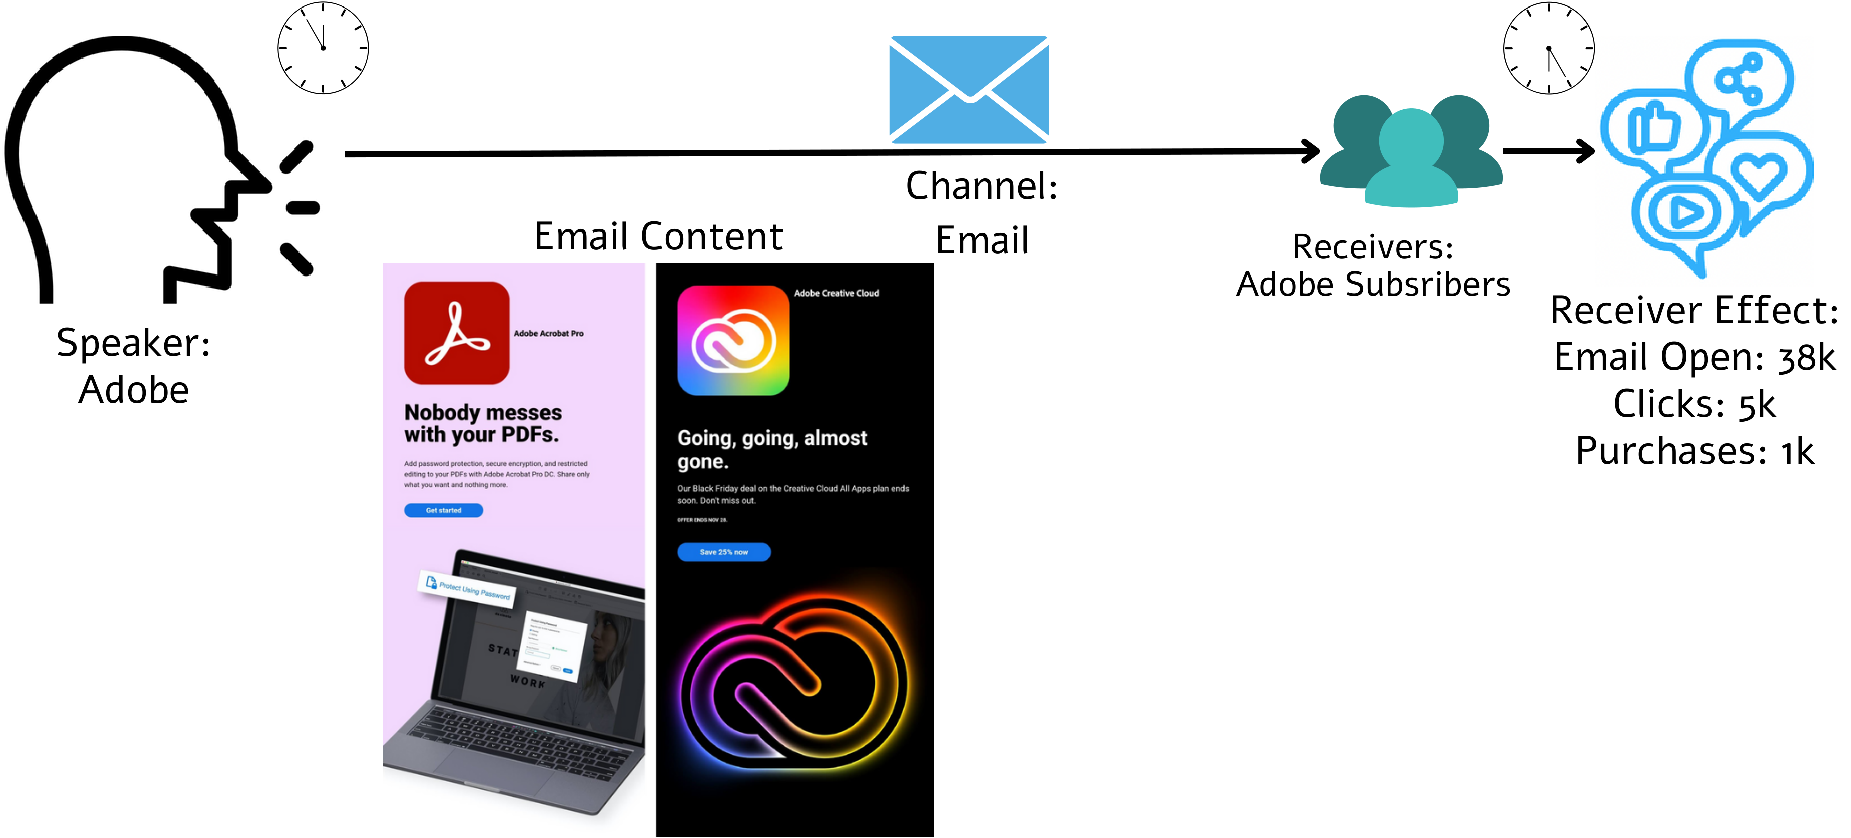
\includegraphics[width=1.0\textwidth]{images/factors of communication.pdf}
  \caption{Communication process can be defined by seven factors: Communicator, Message, Time of message, Channel, Receiver, Time of effect, and Effect. Any message is created to serve an end goal. For marketers, the end goal is to bring in the desired receiver effect (behavior) (like clicks, purchases, likes, and customer retention). The figure presents the key elements in the communication pipeline - the marketer, message, channel, receivers, and finally, the receiver effect. \label{fig:factors-of-communication-chapter-lcbm}}
\end{figure*}


Another possible way to integrate behavior with text is an encoder approach, which we will detail next. While behavior is a downstream effect of content, behavior contains signals about the content sent to the receiver and can help improve content-understanding and natural language processing. For instance,  integration of human gaze data into neural network architectures has been explored for a range of computer vision tasks such as image captioning, visual question answering, and tagging \cite{karessli2017gaze,yu2017supervising,he2019human,boyd2022human}. In language processing, tracking a reader's eye movements provides information about the cognitive processes of text comprehension \cite{RaynerReadingComp, Just1980}. Hence, recent research has utilized features gleaned from readers' eye movement to improve the performance of complex NLP tasks such as sentiment analysis \cite{long-etal-2017-cognition, mishra-etal-2016-leveraging}, sarcasm detection \cite{mishra-etal-2016-harnessing}, part-of-speech tagging \cite{barrett-etal-2016-cross}, NER \cite{hollenstein-zhang-2019-entity}, and text difficulty \cite{ScanPathApp1}. While these studies show promise that behavior can be used to extract information about content, these are done in relatively small-scale lab settings needing real-time behavior to infer about content. Given these limitations, these approaches are not possible to scale. Scale helped LLMs to learn language. We therefore explore the paradigm of synthetic behavior generated over content and then scale it over to fine-tune a large language model to understand the possibilities of this paradigm better. We cover both the approaches next.





%%%%%%%%%%%%%%%%%%%%%%%%%%%%%%%%%%%
%%%%%%%%%%%%%%%%%%%%%%%%%%%%%%%%%%%

\section{Large Content and Behavior Models (LCBM)}
\label{sec:Large Content and Behavior Models (LCBM)}
In this work, we explore the paradigm of the effectiveness problem as a text-to-text problem. The problem of effect is to know what the receiver does after receiving the message \cite{shannon-weaver-1949}. In general, for a piece of content, other than the content itself, we often have information about \textit{who} consumes the content and what his \textit{action} is on consuming the content. The latter is the effect described in Shannon's three levels of communication. For instance, an email, as a message from the communicator to the receiver, elicits certain actions from the receiver like link-clicks, replies, and read-time. While LLMs are trained on trillions of tokens of content, the training does not include the receiver effect. For instance, Enron Email \cite{klimt2004enron} is a popular corpus that is included in the training of LLMs like Pythia \cite{biderman2023pythia}. It contains 600K email content sourced from the Enron corporation, which LLMs use to learn how to write emails. However, it does not contain data about the receivers' activities, such as whether they opened the email, how long they kept it open (read-time), and what their reply was. Similarly, while major text corpora include a large number of public blogs and user forums to train LLMs like CommonCrawl, they are stripped of receiver behavior on forum messages, such as the number of likes, shares, and replies, before including them in LLM training (for instance, see \cite{biderman2022datasheet,penedo2023refinedweb}). 
To pose the effectiveness problem as a text-to-text problem, we can include these \textit{behavior tokens} in the text along with content tokens and train the LLM to model both of those in the same space. This might help the LLM simulate the receiver effect, optimize for it, and reason about it. 





\begin{figure*}[!ht]
    \centering
    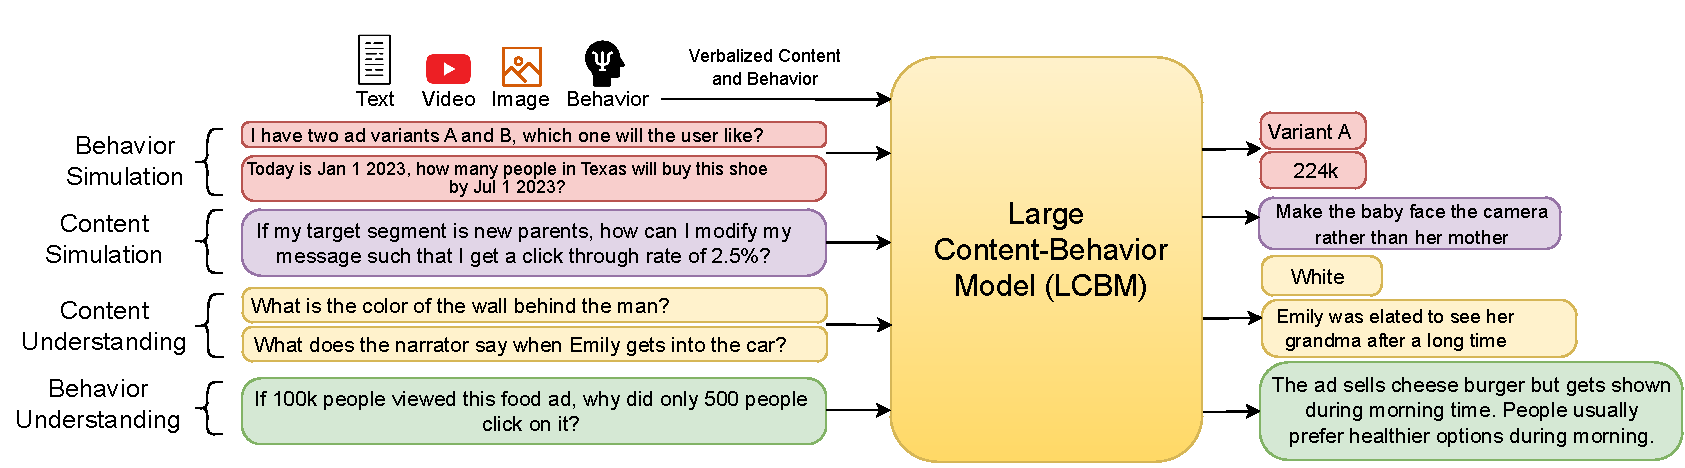
\includegraphics[width=\textwidth]{images/fig1-lcbm.pdf}
    \caption{Encoding and predicting content (images, videos, and text) and behavior in the language space. Large Content Behavior Models (LCBMs), once trained, can enable a host of different applications, including behavior simulation, content understanding, content-behavior optimization, and content-behavior understanding.}
    \label{fig:figure-1-lcbm}
\end{figure*}

\begin{figure*}[!t]
\centering
\makebox[\textwidth]{%
\resizebox{1.0\textwidth}{!}{%
\begin{subfigure}[b]{0.4\textwidth}
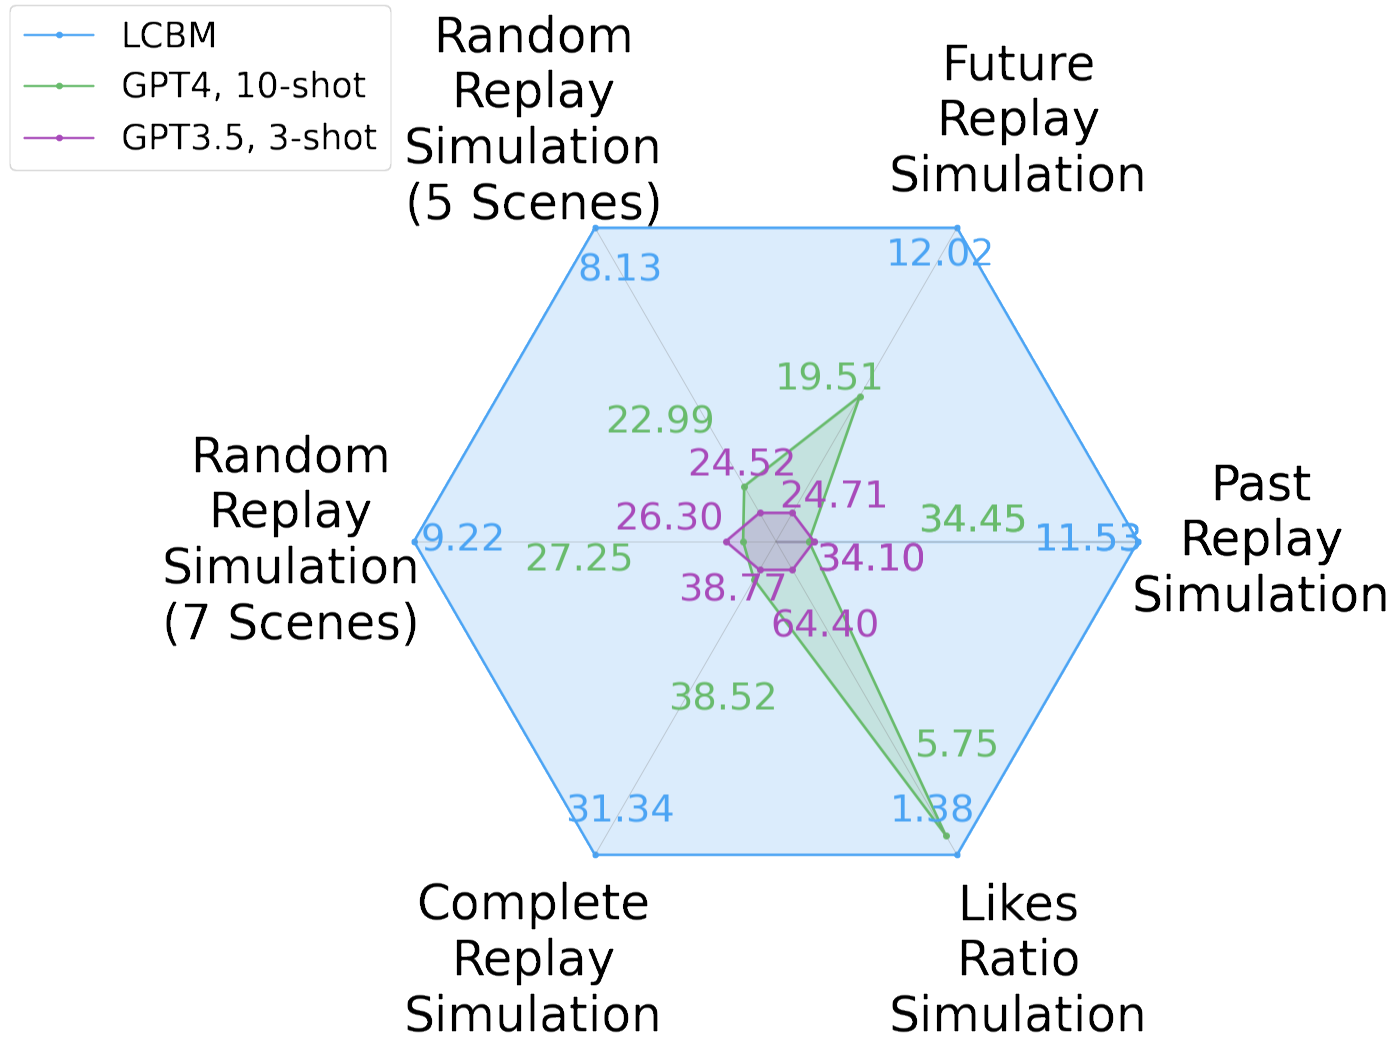
\includegraphics[width=1.15\textwidth]{images/r2_score.png}\caption{}    
\end{subfigure}
\begin{subfigure}[b]{0.4\textwidth}
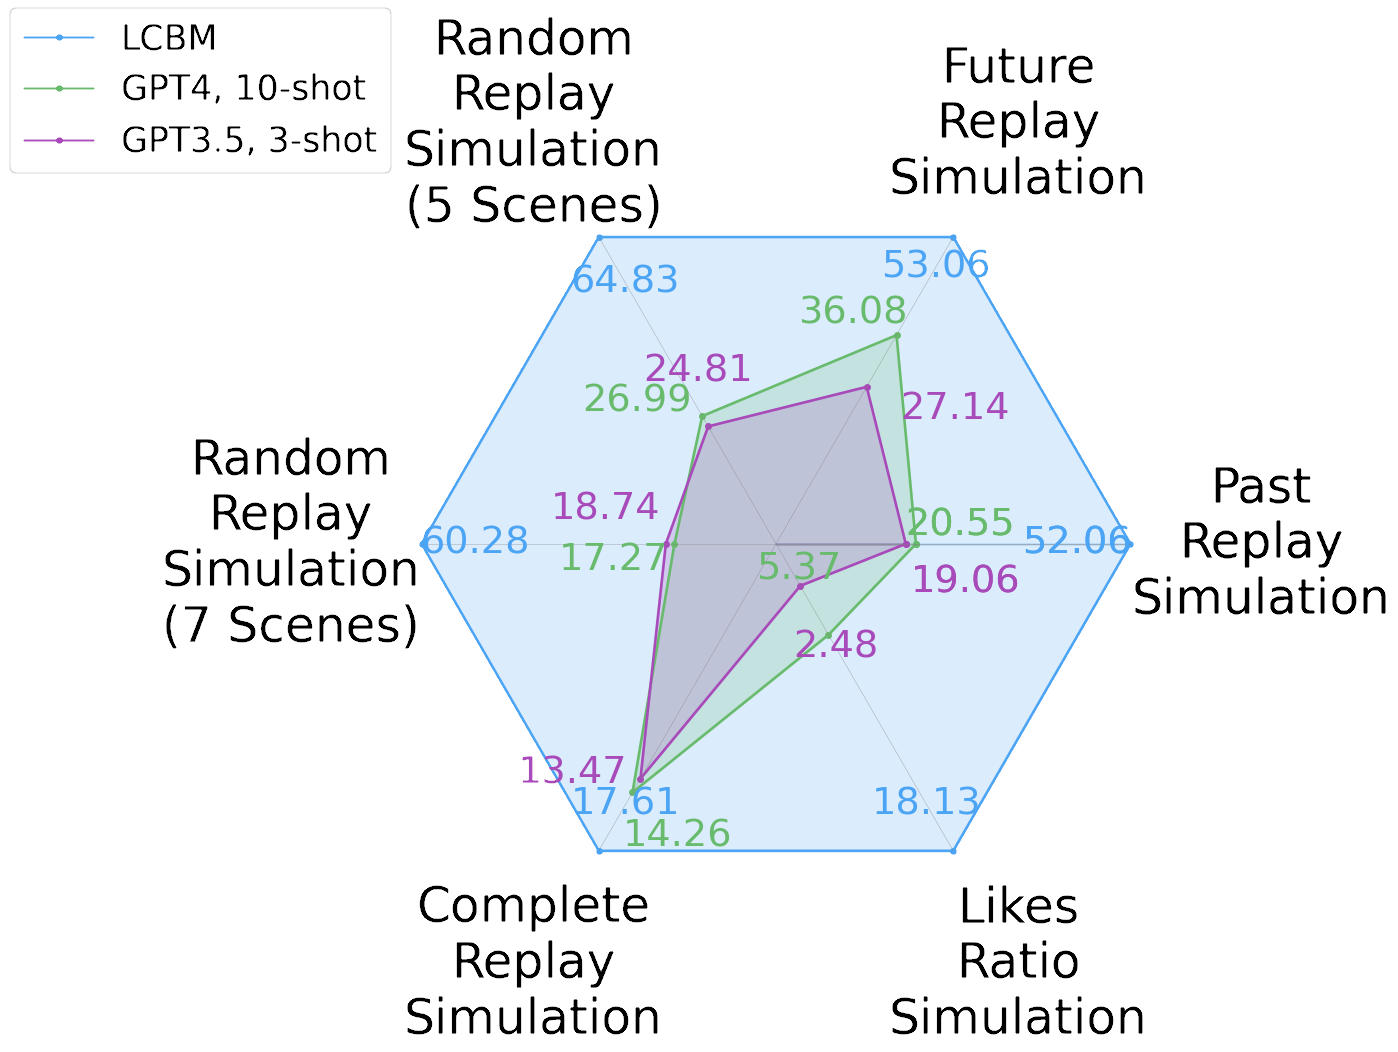
\includegraphics[width=1.15\textwidth]{images/accuracy_2.png}\caption{}    
\end{subfigure}
%\includegraphics[width=0.25\textwidth]{images/behavior-simulation-2-radar-plot.pdf}\caption{}
\begin{subfigure}[b]{0.4\textwidth}
    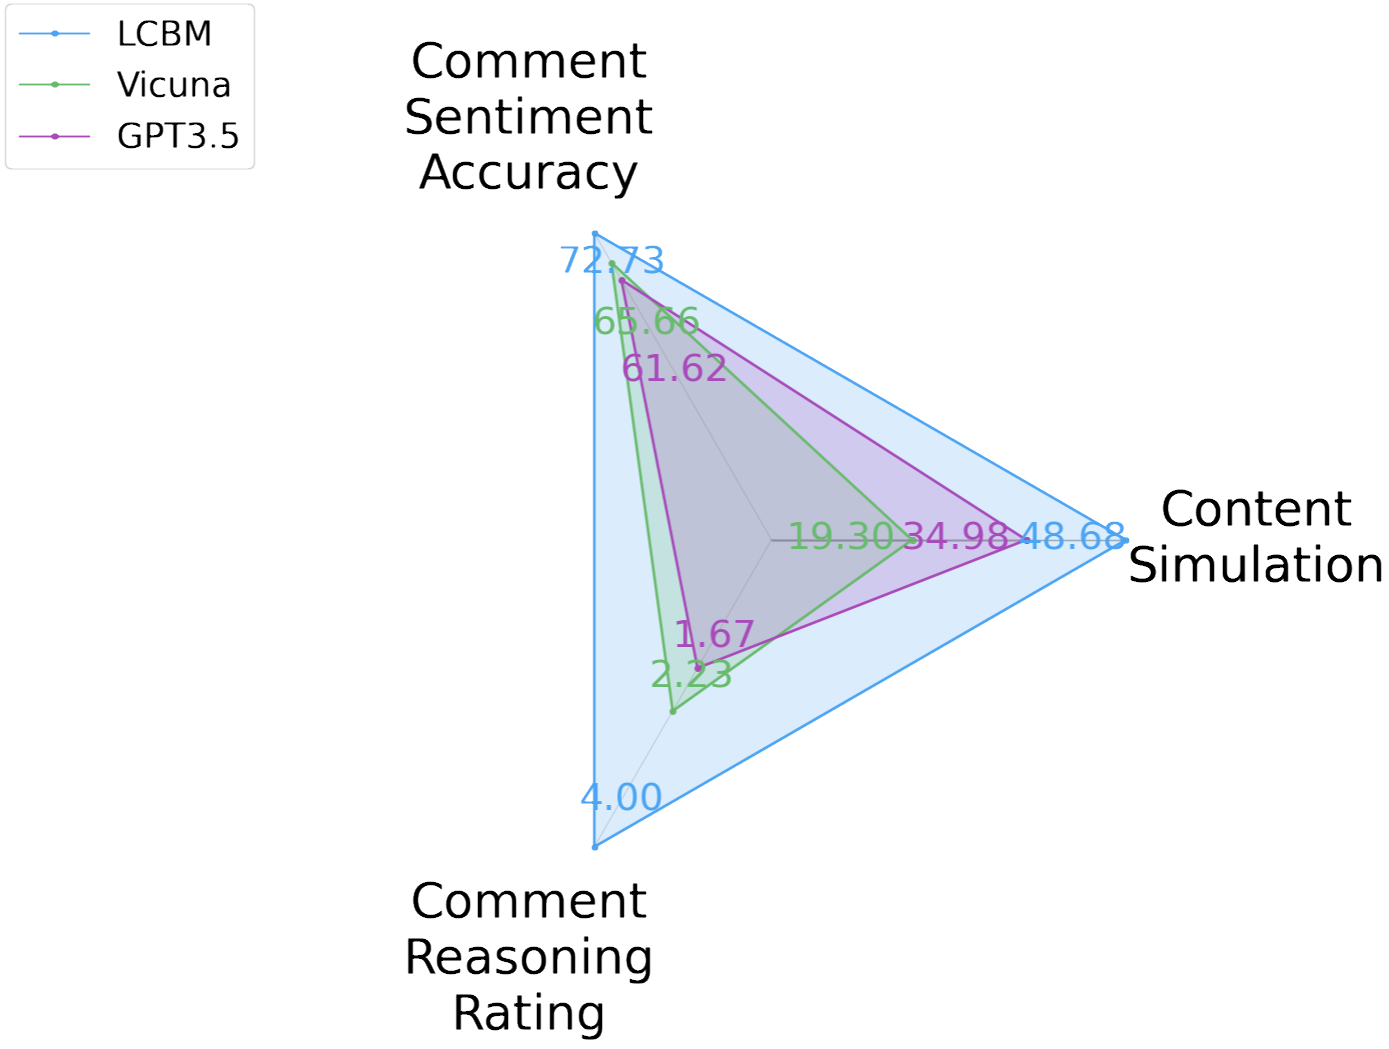
\includegraphics[width=1.15\textwidth]{images/content_simulation_2.png}
    \caption{}
\end{subfigure}
\begin{subfigure}[b]{0.4\textwidth}
    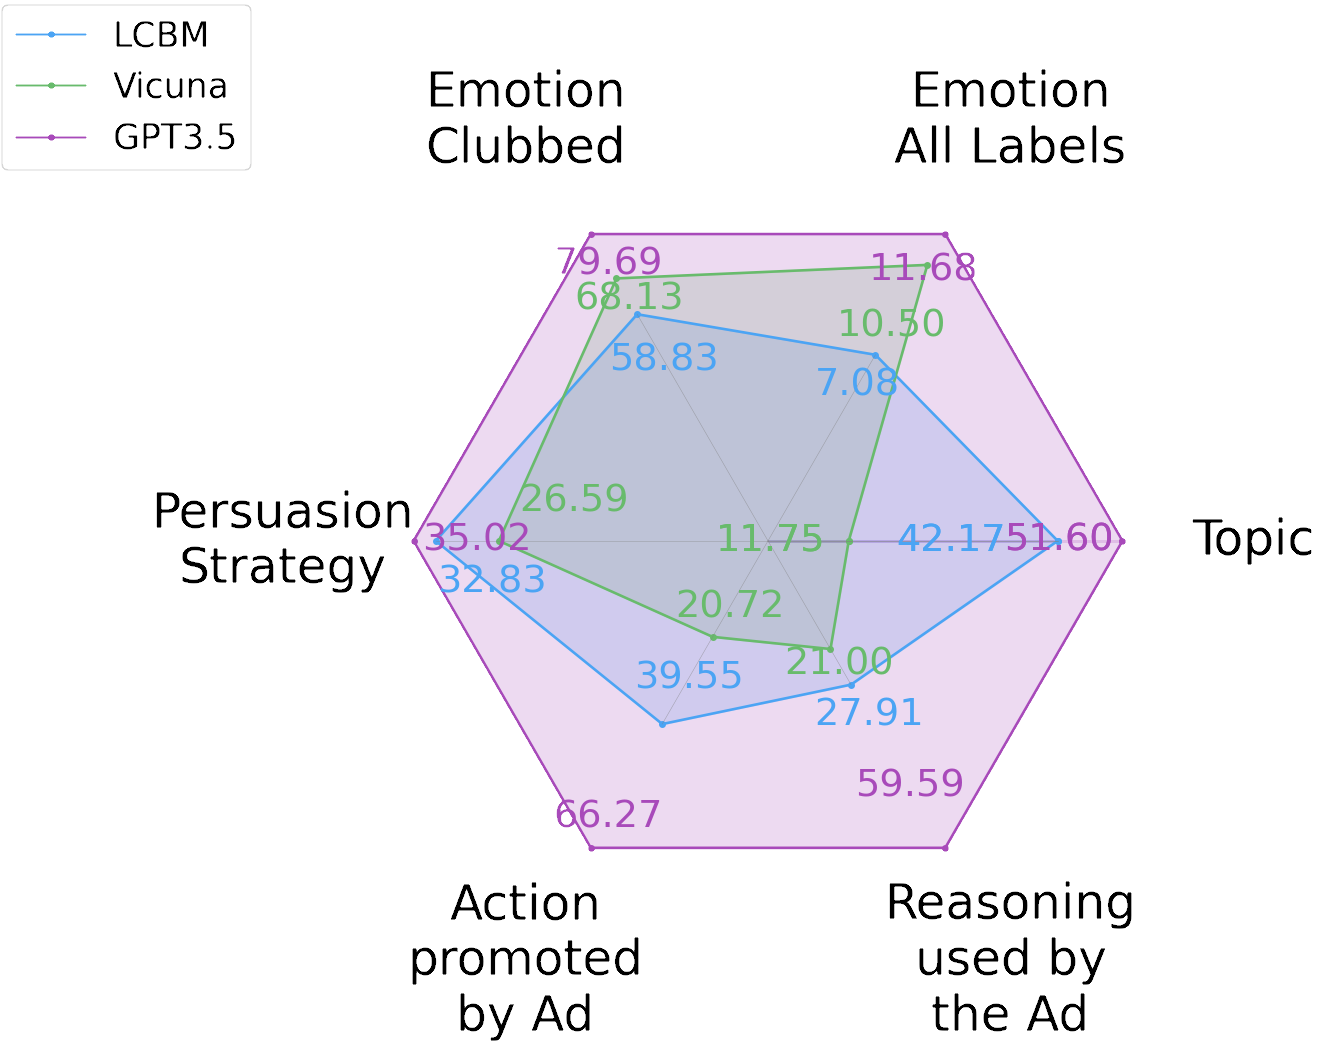
\includegraphics[width=1.15\textwidth]{images/understanding_2.png}
    \caption{}
\end{subfigure}
\iffalse
\begin{subfigure}[b]{0.25\textwidth}
\includegraphics[width=1\textwidth]{images/rmse_scores_final.pdf}\caption{}    
\end{subfigure}
\begin{subfigure}[b]{0.25\textwidth}
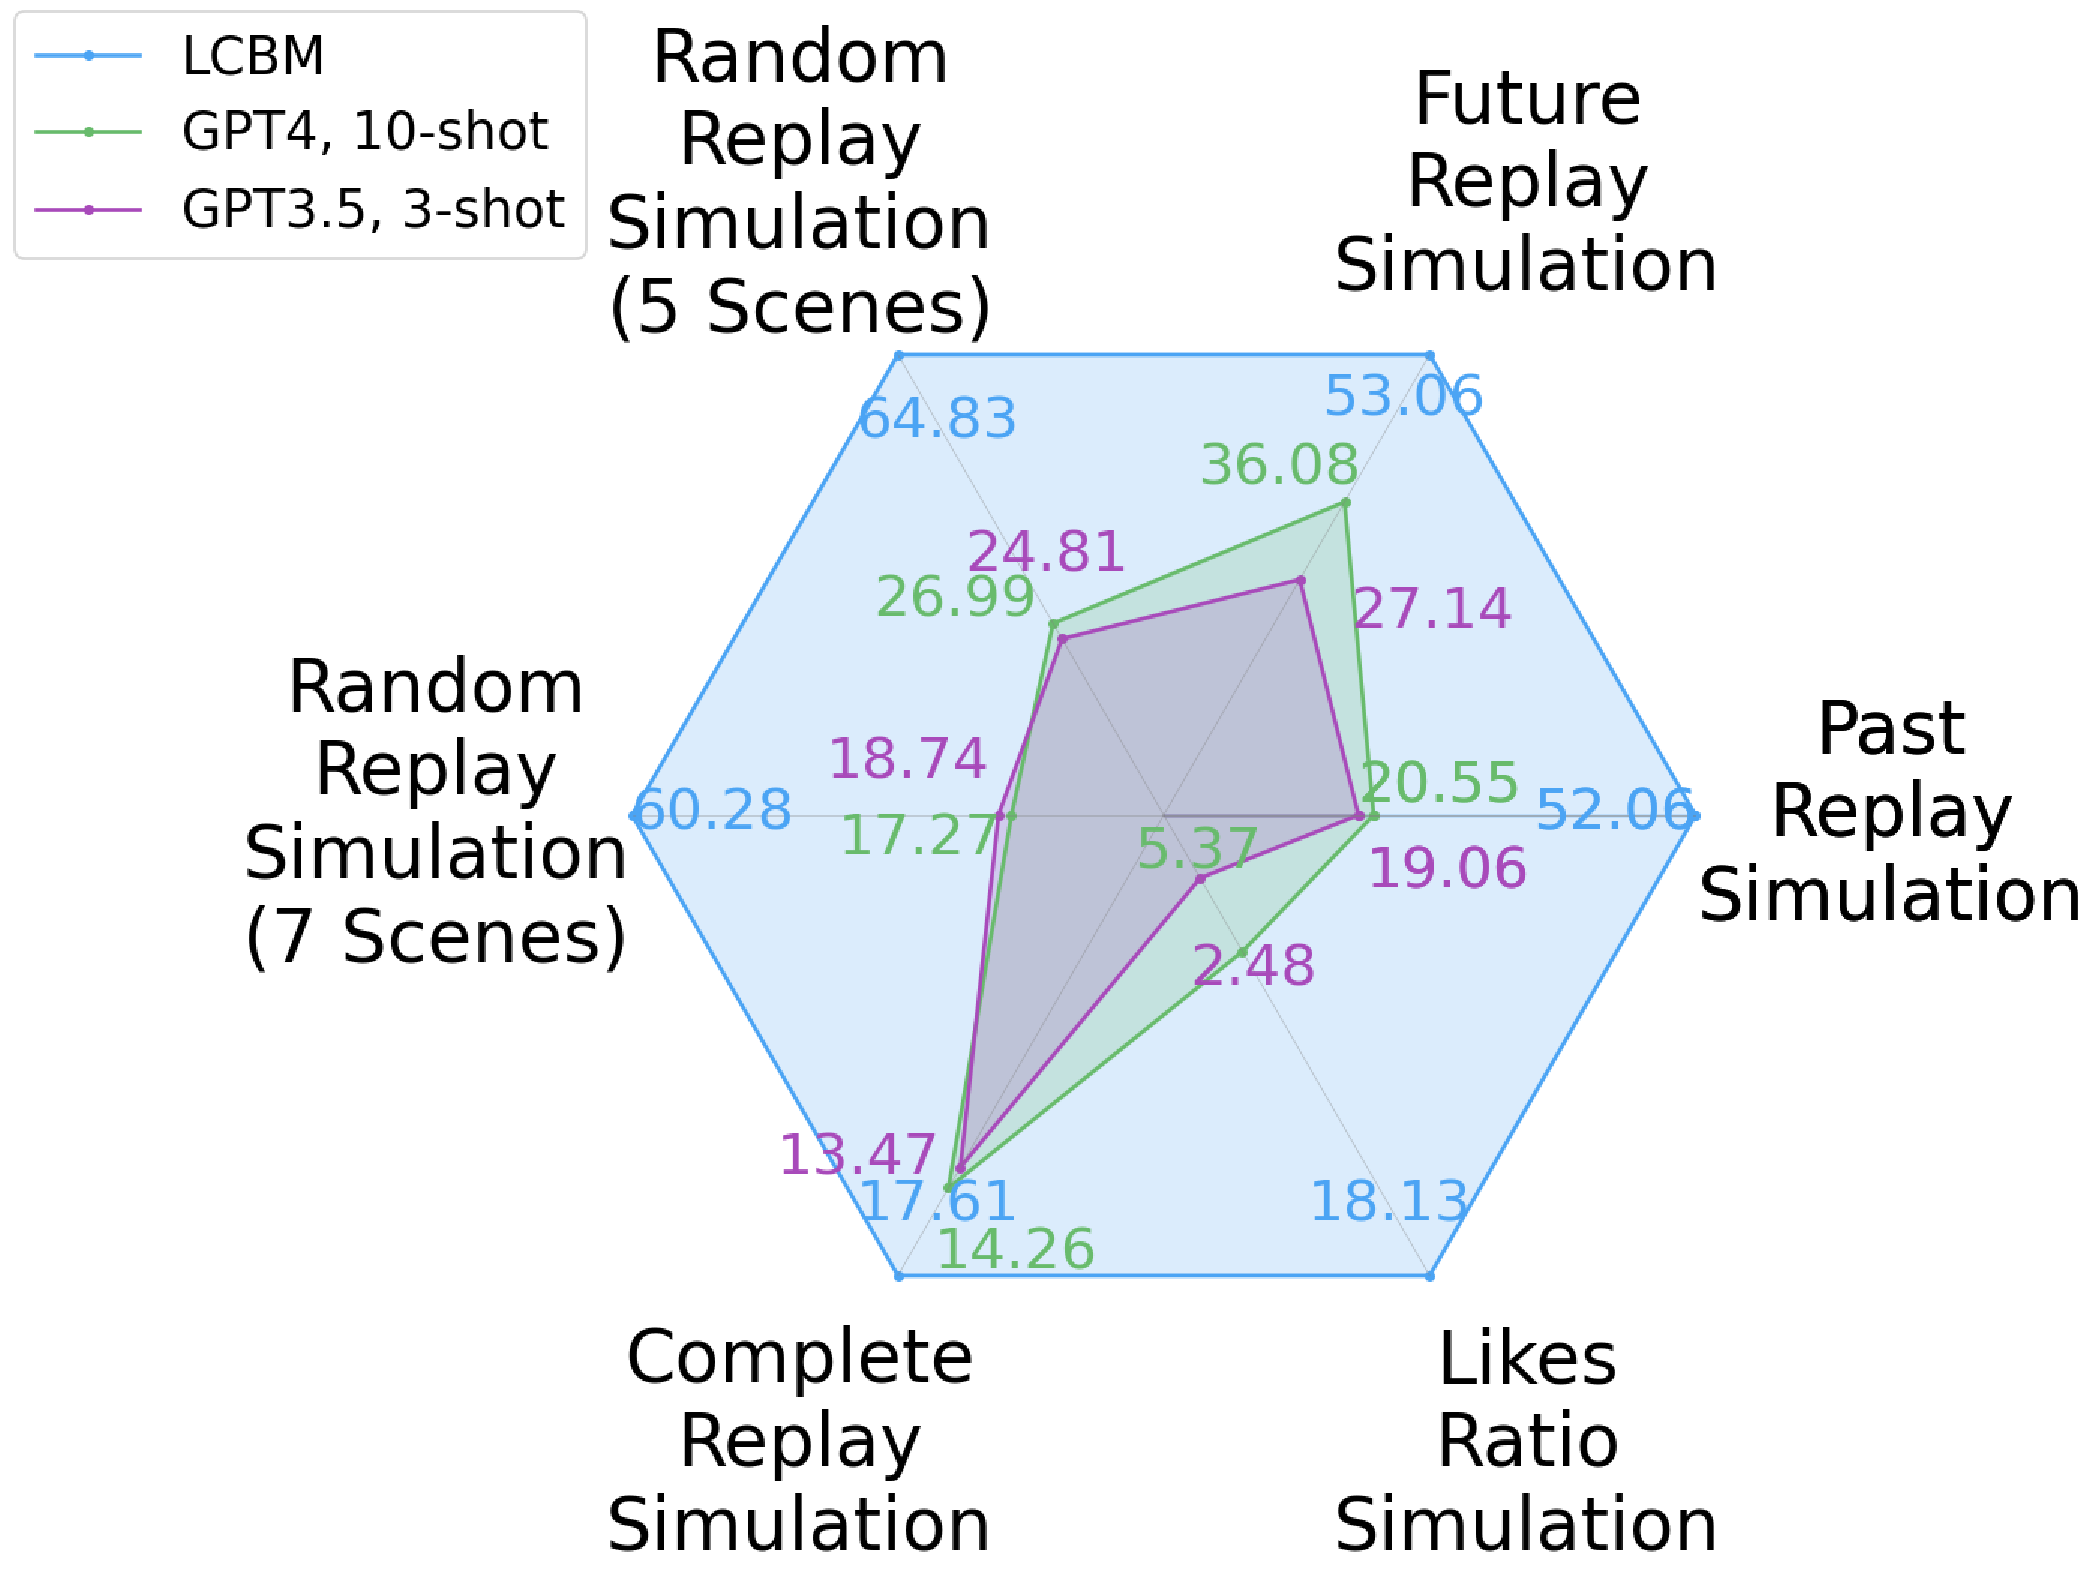
\includegraphics[width=1\textwidth]{images/accuracy_scores_final.pdf}\caption{}    
\end{subfigure}
%\includegraphics[width=0.25\textwidth]{images/behavior-simulation-2-radar-plot.pdf}\caption{}
\begin{subfigure}[b]{0.25\textwidth}
    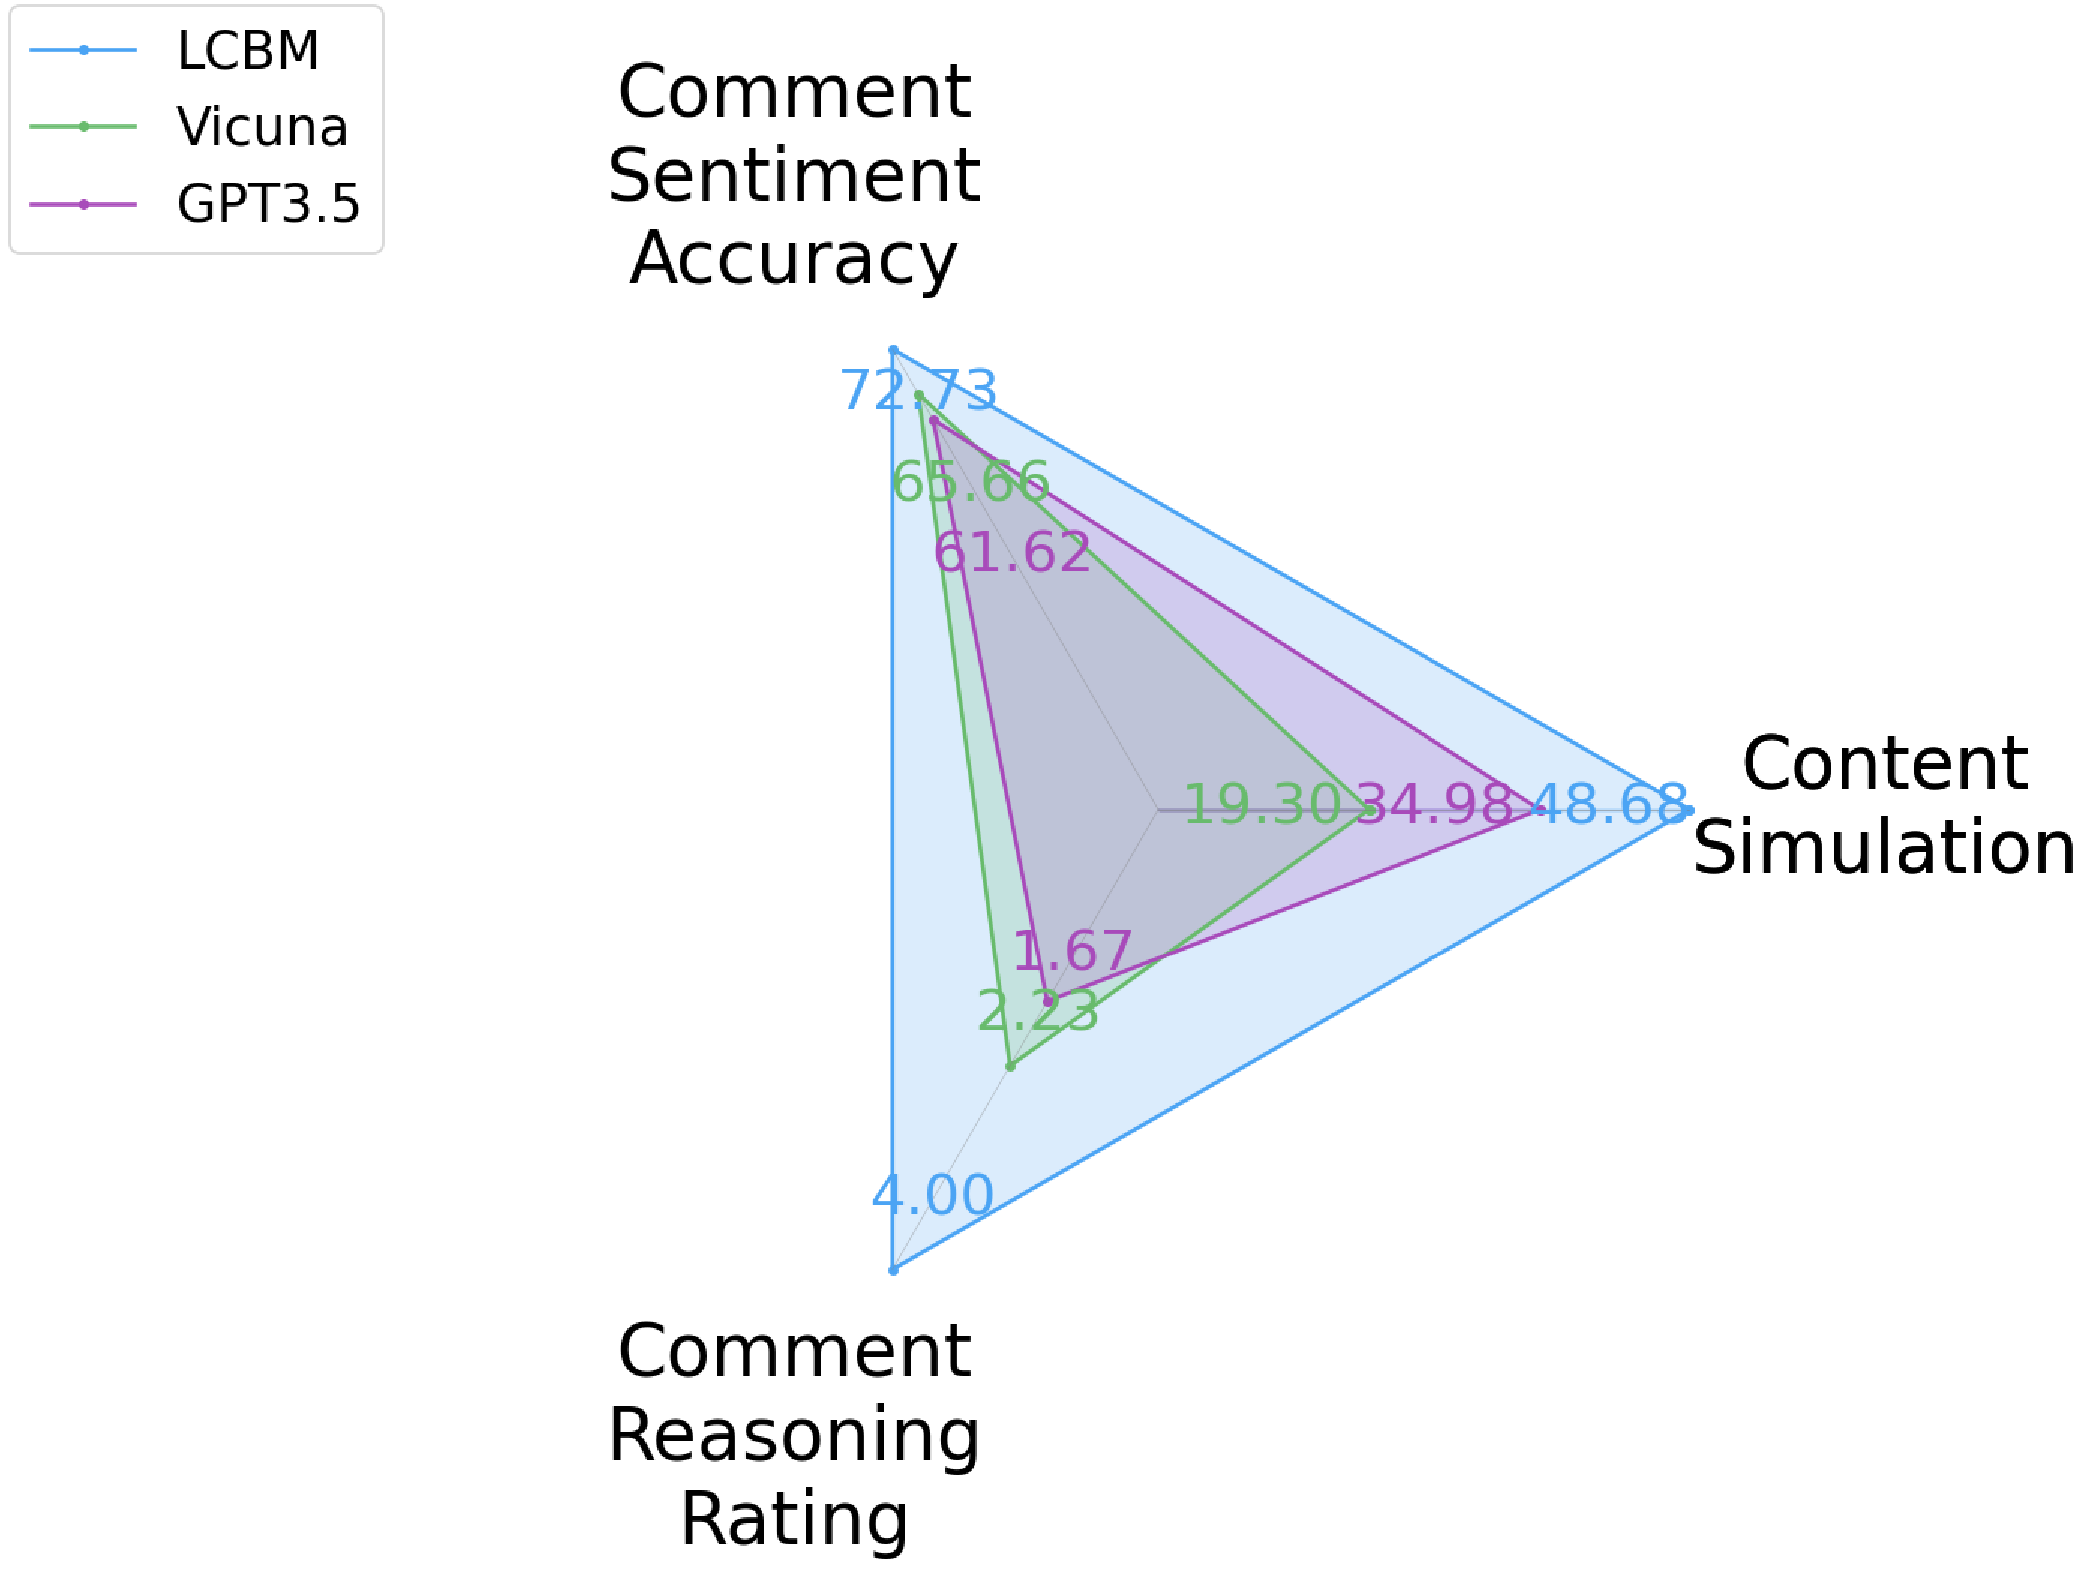
\includegraphics[width=1\textwidth]{images/content_simulation_scores.pdf}
    \caption{}
\end{subfigure}
\begin{subfigure}[b]{0.24\textwidth}
    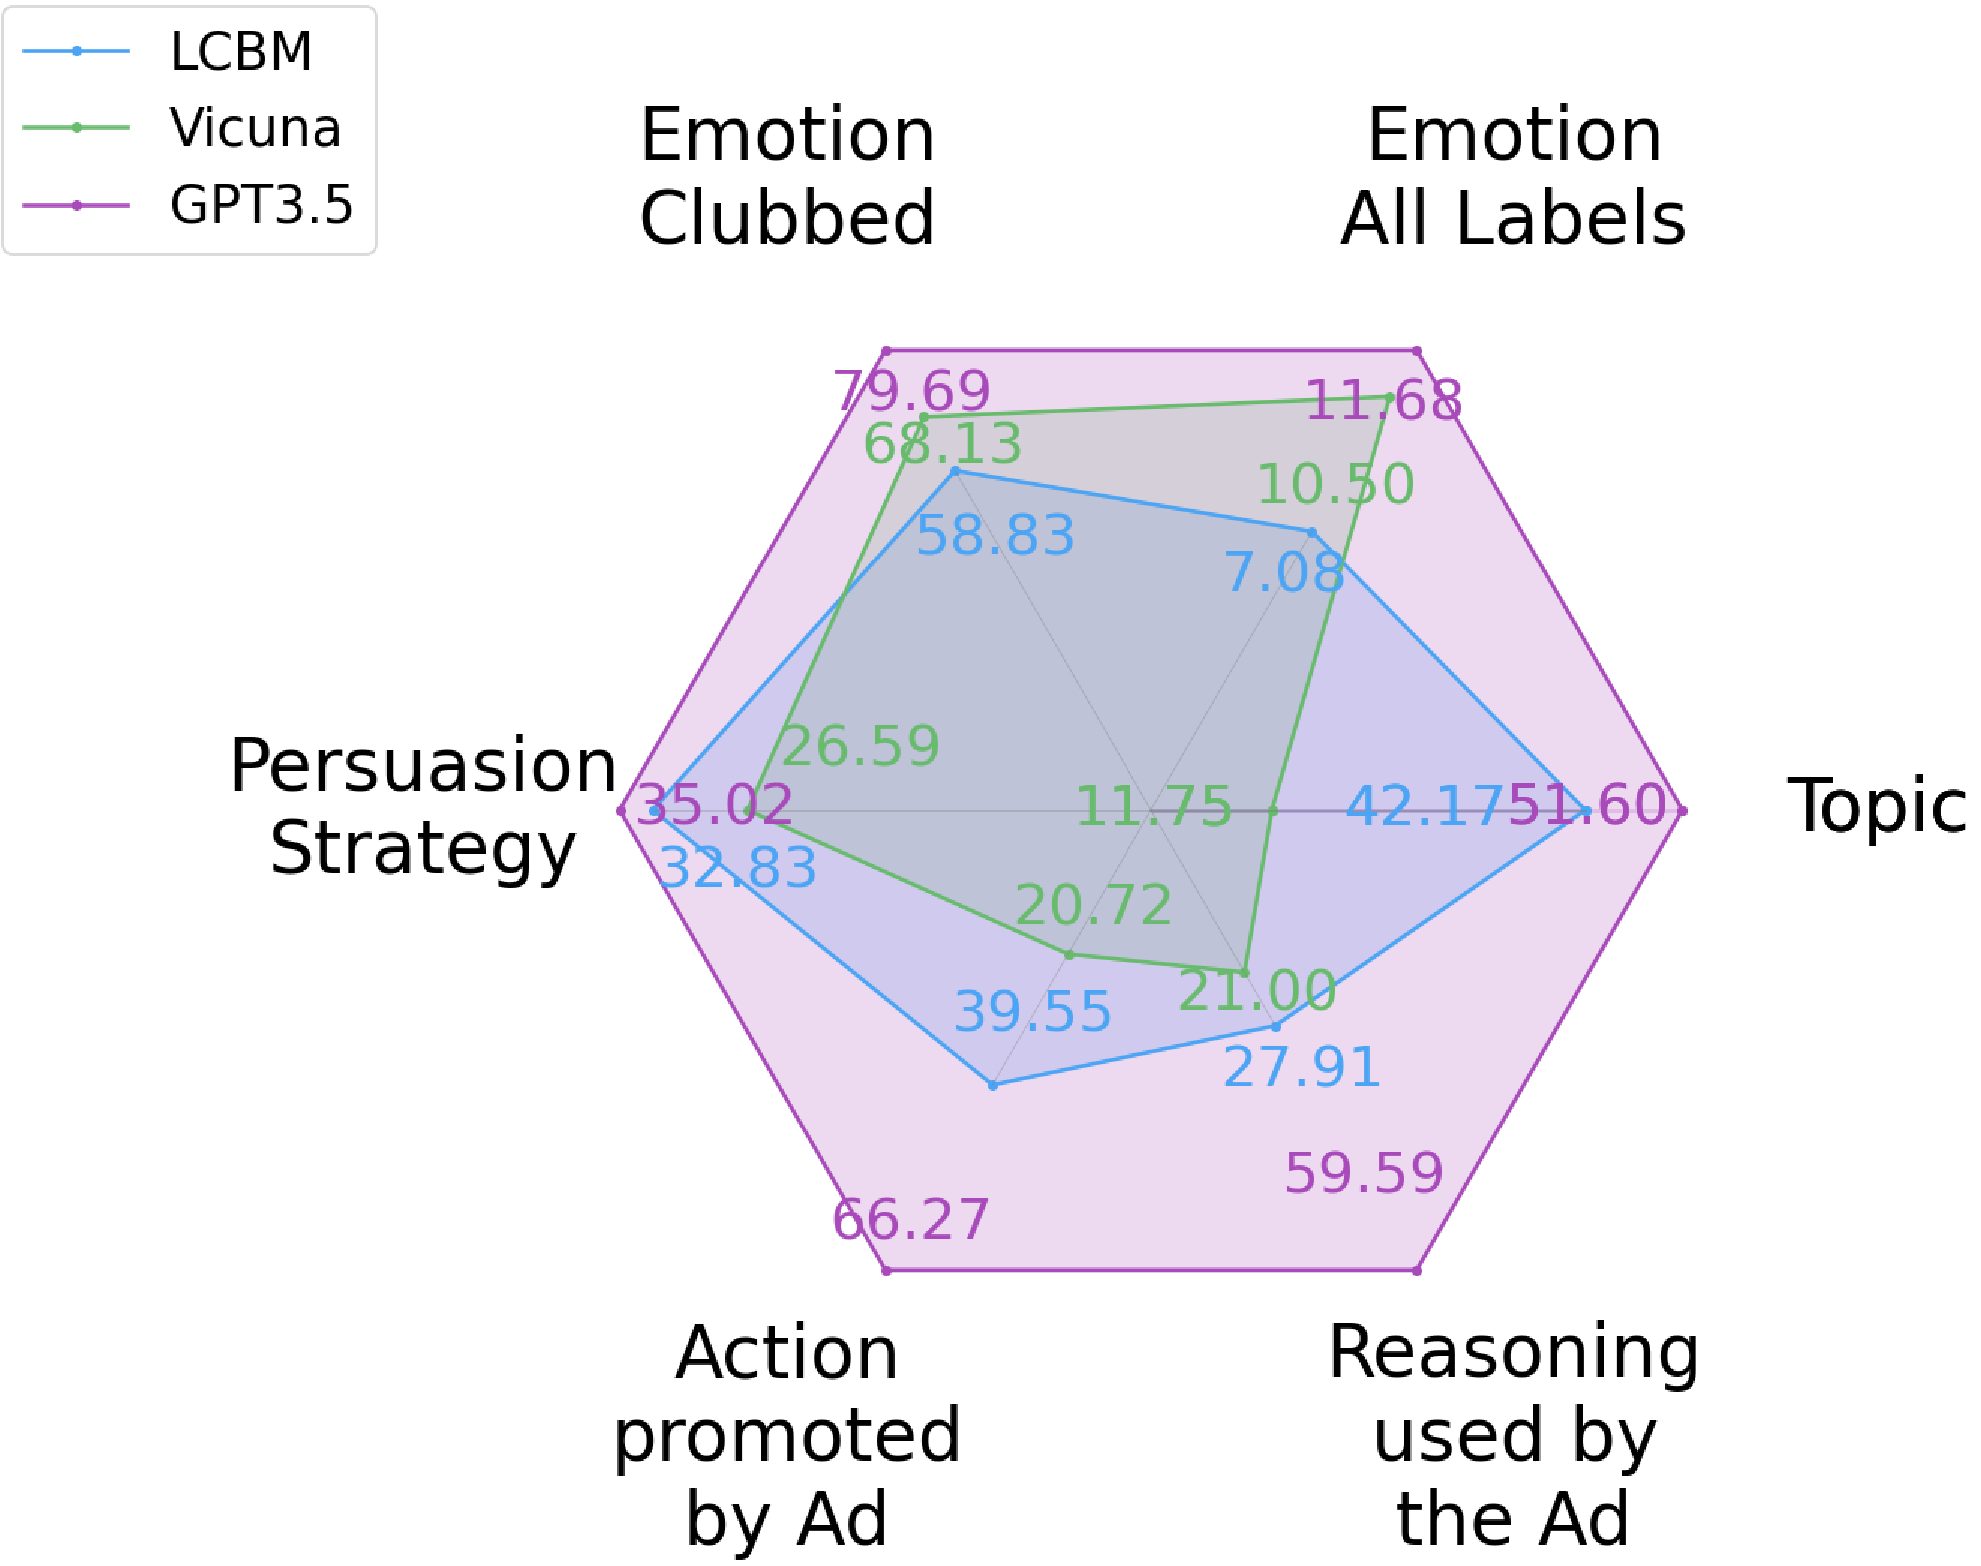
\includegraphics[width=1\textwidth]{images/content_understanding_scores.pdf}
    \caption{}
\end{subfigure}
\fi
}}
    \caption{
    \label{fig:capabilities-radarplot}
    Comparison of GPT-3.5, GPT-4, Vicuna-13B, and LCBM-13B on ((a),(b))~Behavior Simulation on two types of behaviors: replay value prediction and likes/views prediction. The task is, given the video content and channel information, to predict replay values corresponding to each scene and the ratio of likes to views. (a)~is the negative RMSE scores, and (b)~is the accuracy.
    (c)~Content simulation and behavior understanding tasks. The task for content simulation is, given the channel information and scene-level behavior, to predict the scene content. Given information on the video platform and the video content, the task of behavior understanding is to predict and explain the sentiments of the viewers and the commenters. %The predicted sentiment is compared with the average ground truth sentiment of all the YouTube comments. 
    Six evaluators scored the models' explanations between 0-5 to get the predicted sentiment and explanation scores by comparing the ratings and reasons with the user comments. The annotators did not know which model gave the reasoning.
    (d)~Content understanding tasks. We evaluate four tasks: emotion, topic, and persuasion strategy prediction, and action-and-reason understanding. It can be noted that on the behavior simulation, content simulation, and behavior understanding tasks, LCBM performs better than 3-shot GPT-3.5 and 10-shot GPT-4 (covering a larger area. On the content understanding tasks, while LCBM outperforms similar-sized Vicuna models, GPT-3.5 performs better. However, we also note that GPT-3.5 and GPT-4 are at least 12 times larger than LCBM-13B. Further, we show the behavior domain adaptation results in Table~\ref{table:behavior-domain-adaptation}.
    %Keeping a cutoff R2 Score of -1.25, GPT-3.5 was excluded due to its, poor performance, (c)
    }
\end{figure*}







%This makes LLM unable to simulate behavior and optimize content for a particular audience effect. Therefore, the natural next step is to include behavior tokens in LLM training to teach it the behavior modality\footnote{Here, we take the view of modality as defined as by \citet{lahat2015multimodal}, where they define it as phenomena captured using multiple independent sensors and each sensor output can be termed as a modality \cite{ramachandram2017deep}.}. However, training an LLM from scratch is expensive. 

%Communication as defined by the communication theorist, Harold Lasswell, is  by five factors: who (\textit{i.e.}, communicator) says what (\textit{i.e.}, message) through which medium to whom (\textit{i.e.}, the receiver) and with what effect (\textit{i.e.}, behavior) \cite{}. Therefore, to capture communication in its entirety, we need to model all five factors of communication. However, large language models are trained only on (at most) three factors among the five factors: communicator, message, and receiver. The behavior modality additionally defines how the receiver will act while interacting with the content, and what attitude and action changes are observed in the receiver after that. 

%Recently, a few studies have shown that instruction fine-tuning makes it possible to teach LLMs a new modality. They rely on the assumption that language semantics can play a wider role: a universal interface representing all modalities in the language space. Examples like GPT-4 \cite{openai2023gpt4}, BLIP \cite{li2023blip}, Llava \cite{liu2023visual}, and Video4096 \cite{bhattacharya2023video} demonstrate this power of LLMs. Therefore, following them, we teach an LLM the behavior modality using instruction fine-tuning, thus helping it learn to solve the Level C proposed by \citet{shannon-weaver-1949}. We call this instruction fine-tuning, behavior tuning of the model.

%As per Laswell's model of communication, these modalities represent the message and aspects of the channel, but miss out on a crucial modality, the behavior modality. A model trained on all the five factors will be able to simulate a receiver's behavior, would be able to help the communicator optimize its message to elicit certain receiver behavior, and also explain the reason for receiver's behavior. 



In this work, we show initial experiments to integrate behavior as a new modality to increase the scope of multimodal LLMs from only content to both content and behavior. We call this new type of model a Large Content Behavior Model (LCBM). This class of models shows promise in enabling the LLMs to not only reason about content but also reason about and predict human behavior over that content. Further, LCBMs have the potential for behavior domain adaptation where models trained on one type of behavior can generalize on another behavior type (Fig.~\ref{fig:capabilities-radarplot}). Behavior simulation can enable many real-world applications, such as content recommendation, customer journey optimization, and A/B testing. To build LCBM, we introduce behavior instruction tuning (\S\ref{sec:behavior-instruction-tuning}), an attempt to extend the instruction tuning paradigm to behavior space, bringing all seven communication factors (communicator, message, channel, receiver, send time, receive time, and effect) into the same space (Fig.~\ref{fig:factors-of-communication-chapter-lcbm}). Similar to \cite{brown2020language,raffel2020exploring,liu2023visual,ge2023planting}, we do not design best-in-class predictors for any of the downstream tasks. Rather, we show a model which shows generalization capabilities across a wide variety of content- and behavior-related tasks. To summarize, we make the following two contributions:

\begin{itemize}[leftmargin=*]
    \item\textbf{Large Content Behavior Model (LCBM).} We develop a large multimodal model that shows capabilities of behavior simulation (given content), content simulation (given behavior), content understanding, and behavior understanding (Fig.~\ref{fig:figure-1-lcbm}). Following the text-to-text framework, we connect the Vicuna LLM \cite{touvron2023llama,vicuna2023} with an open-set visual encoder of EVA-CLIP \cite{sun2023eva} and instruction fine-tune it end-to-end on behavior instruction data. EVA-CLIP and QFormer \cite{li2023blip2} help the model to understand visual content in the language space, making it a Vision Language Model (VLM). During behavior instruction tuning, we teach the model to predict behavior given content and content given behavior using various instruction tasks (\S\ref{sec:behavior-instruction-tuning}). This helps us teach behavior modality to the VLM while grounding it in the natural language space. We use three datasets to show the performance of LCBM: a dataset consisting of YouTube videos as the content and the corresponding retention graph, likes, the number of views, and comment sentiment as receiver behavior; a dataset consisting of Twitter posts (text, images, and videos) and corresponding human behavior (like counts) extracted from 168 million tweets across 10135 enterprise Twitter accounts from 2007 to 2023; and an internal dataset of \companyName Marketing Emails\footnote[6]{We obtain \companyName Marketing Emails dataset by collaborating with the \companyName team.} (content) and the click-through rate corresponding to each segment they were sent to (behavior). We observe that teaching the LCBM behavior and content simulation improves its capabilities on them (expected), but the model also shows signs of domain-adaptation in behavior modality (few-shot capability, \textit{unexpected}) (Tables~\ref{table:behavior-domain-adaptation}, \ref{table:behavior-simulation-like-simulation-twitter}, \ref{table:content-simulation-twitter}) and improvements in behavior understanding (Figs.~\ref{fig:comment-explains}, \ref{fig:replay-explains}, \S\ref{sec:results}) (zero-shot capability, \textit{unexpected}) \cite{brown2020language}. See Fig.~\ref{fig:capabilities-radarplot} for a radar plot of all the capabilities and comparisons of performances across LCBM and state-of-the-art LLMs: GPT-3.5 and GPT-4.

    \item\textbf{Dataset and Test Benchmark.} To spur research on the topic of large content and behavior models, we release our generated behavior instruction fine-tuning data from over 40,000 public-domain YouTube videos and 168 million Twitter posts. The data contains: 1)~YouTube video links, automatically extracted key scenes, scene verbalizations, replay graph data, video views, likes, comments, channel name, and subscriber count at the time of collection, and 2)~Twitter extracted account names, tweet text, associated media (image and video) verbalizations (including image captions, keywords, colors, and tones), tweet timestamps, and like counts. We also release a benchmark to test performance on the joint content behavior space (\S\ref{sec:test benchmark}), introducing two types of tasks in this space: predictive and descriptive. In the predictive benchmark, we test the model's ability to predict behavior given the content and predict content given the behavior. In the descriptive benchmark, we validate its explanation of human behavior by comparing it with ground-truth annotations we obtain from human annotators that try to explain human behavior. See Figs.~\ref{fig:comment-explains}, \ref{fig:replay-explains} for a few examples.
\end{itemize}



%To the best of our knowledge, ours is the first effort in the LLM space to bring content and behavior into the same space. 
%Our empirical results validate the effectiveness of using content-behavior data for LLM instruction tuning and suggest practical tips for building a model which can model both content and human behavior in the same space. Concretely, we model content and behavior modalities together for image and video datasets across four different types of behavior metrics across four tasks in the benchmark tested across three LLMs.
%Teaching an LLM to use its world knowledge to reason about content and simulate behavior can enable many applications, including content optimization (for \textit{e.g.}, forecasting the number of clicks for marketing emails before they are released), A/B testing (for \textit{e.g.}, and testing which variant of a video will get more likes and views).


%\item 

%\end{itemize}




\subsection{Setup}
\label{sec:Setup}
In this section, we introduce our approach to model content and behavior together as a text-to-text problem. Since most publicly available corpora strip off receiver behavior from content, we first introduce our dataset, ``The Content Behavior Corpus (CBC)'', a dataset consisting of content and the corresponding receiver behavior. Next, we introduce our methodology to convert the content and behavior into text and our approach to model it using an LLM. Then, we cover the tasks through which we test various capabilities of LCBM (Fig.~\ref{fig:figure-1-lcbm}): content-understanding, behavior understanding, content simulation, behavior simulation, and behavior domain adaptation. 


\begin{figure*}[!t]
\centering
    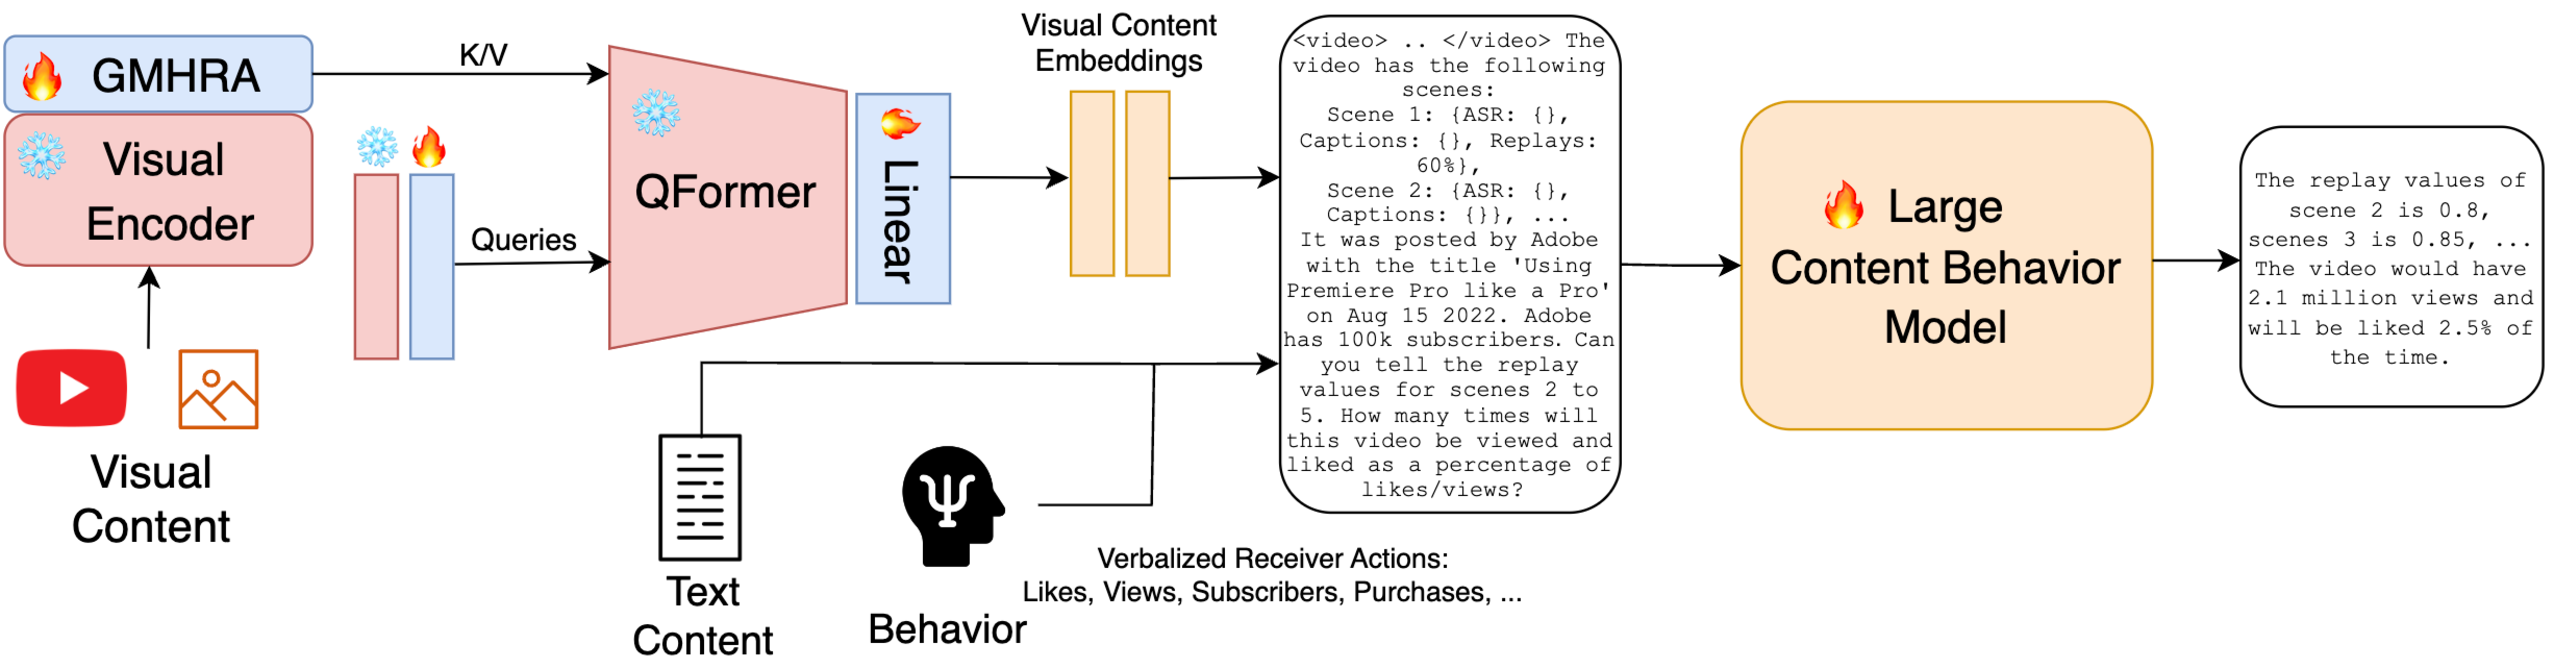
\includegraphics[width=\textwidth]{images/content-behavior-architecture.pdf}
    \caption{Encoding and predicting content (images, videos, and text) and behavior in the language space. Strategy to behavior instruction fine-tune (BFT) LLMs to create LCBMs. We capture visual concepts through the visual encoder (EVA-CLIP), and world knowledge is through an LLM (Llama). To leverage the rich knowledge of LLMs, we use GMHRA and QFormer to convert visual tokens of ViT to language tokens that Llama can understand. Further, we find that verbalizing the visual stimulus helps Llama to gather information more explicitly than what is provided by ViT+QFormer. We fine-tune the combined model end-to-end to predict 1)~behavior given content and 2)~content given behavior. Snowflake and fire symbols denote the frozen and unfrozen parts of the architecture. \cy{What is the frozen value of the query input to QFormer?}}
    \label{fig:lcbm-architecture}
\end{figure*}



\subsection{The Content Behavior Corpus (CBC)}
\label{sec:content behavior corpus}
The availability of large-scale unlabeled text data for unsupervised learning has fueled much of the progress of LLMs. In this work, we are interested in modeling content and the corresponding receiver behavior in the same space. While available datasets contain trillions of content tokens (text, images, audio, and videos), they unfortunately do not contain the receiver effect. To address this, we utilize YouTube and Twitter, two large publicly available sources of content-behavior data, consisting of (a)~account name, account description, and number of subscribers and followers (\textit{communicator data}), (b)~rich content in the form of videos, images, creator-provided captions, titles, and descriptions (\textit{message}), (c)~behavior in the form of likes, views, user comments, and replay graph (\textit{receiver effect}). This covers all the seven factors of communication (Fig.~\ref{fig:factors-of-communication-chapter-lcbm}), with the channel being fixed (as YouTube or Twitter) and receivers being average channel followers and viewers of the communicator. Since content data is multimodal in the form of a combination of images, videos, and text, and behavior data is in the form of numbers, to model it using a text-to-text paradigm, we \textit{verbalize} both of them following the methodology we detail next.


\textit{Verbalization:} For the video $V$, YouTube provides us with 100 average viewer retention values $r_i \text{ for } i\in[0..100)$, corresponding to the entire video. The sampling rate of 100 is constant and independent of video length ($T$). Replay value $r_i$ corresponds to video frames between the timestamps $(T/100\times i, T/100\times(i+1))$, which denotes how often these frames were replayed compared to the most replayed frames. The metric has a value between 0 and 1 that identifies the video's relative retention performance at a given point in the video. To accommodate longer video lengths, we merge replay values until $T/100\times(i+j)-T/100\times i > 1 \text{ second with } j\in\{i+1,100\}$. We choose the replay value for this merged group of scenes as $max(r_i,..., r_j)$. Using this logic, we get replay values $R_i$ for $i \in[0..m]$, where $m=\lfloor 100/(\lceil 100/T \rceil) \rfloor$.
Next, we sample two frames randomly corresponding to each $i \in [0..m]$. We caption the frames using BLIP \cite{li2023blip2}. We also obtain the automatic speech recognition for the speech for the video between the timestamps corresponding to replay value $R_i$ using Whisper \cite{radford2023robust}. The ASR and BLIP captions are content for scenes, and replay values are the behavior corresponding to them. We include the scene content and behavior in the video verbalization (Listing~\ref{lcbm:verbalization}) with the sampling for both scene content and behavior as described above. %\cy{How many scene is that for each video and how to decide that?}
%Let's define a scene $S_i$, consisting of video frames from time $t_i^s,t_i^e$.
%For the scene $S_i$, therefore, the corresponding retention values are $R_i$.  We extract automatic speech recognition (ASR) from the video and BLIP \cite{li2023blip2} generated captions for scenes $S$. Therefore, for a scene $S_i$ spanning time $t_i^s,t_i^e$, we have the following content: scene's ASR, BLIP generated caption, and replay value.

We also include video content by encoding video frames through EVA-CLIP \cite{sun2023eva} (explained in \S\ref{sec:model}). Other than video embeddings, we include the video title and description as part of the video content. Corresponding to the overall video content, we verbalize overall video behavior metrics like video views and the ratio of likes and views. Finally, we append it with communicator information on the video channel and the subscriber count. The Listing~\ref{lcbm:verbalization} presents the overall verbalization for video and frame level content and behavior. The verbalization for Twitter posts is similar and is given in Listing~\ref{listing-twitter-behavior-simulation}.

\begin{lstlisting}[caption={Verbalization pattern for inputting content and behavior in the same space},frame=single,label={lcbm:verbalization},basicstyle=\scriptsize]
Input: <video> ..[Video Tokens] .. </video> 
The video has the following scenes:
Scene 1: {ASR: Welcome to a quick tutorial, OCR: Adobe Premiere Pro, Captions: A desktop interface, Replays: 60}, 
Scene 2: {ASR: on using Premiere Pro to edit, Captions: A computer interface, with an image of a white horse. Objects - Horse, Grass, Fence., Replays: 53}, 
... 
It was posted by Adobe with the title 'Using Premiere Pro like a Pro' on Aug 15 2022. Adobe has 100k subscribers. This video was viewed by 346 thousand people and liked (as a percentage of likes/views) by 2.3% people. 
\end{lstlisting}

\begin{figure}[!t]
\begin{minipage}{\textwidth}
    \centering
    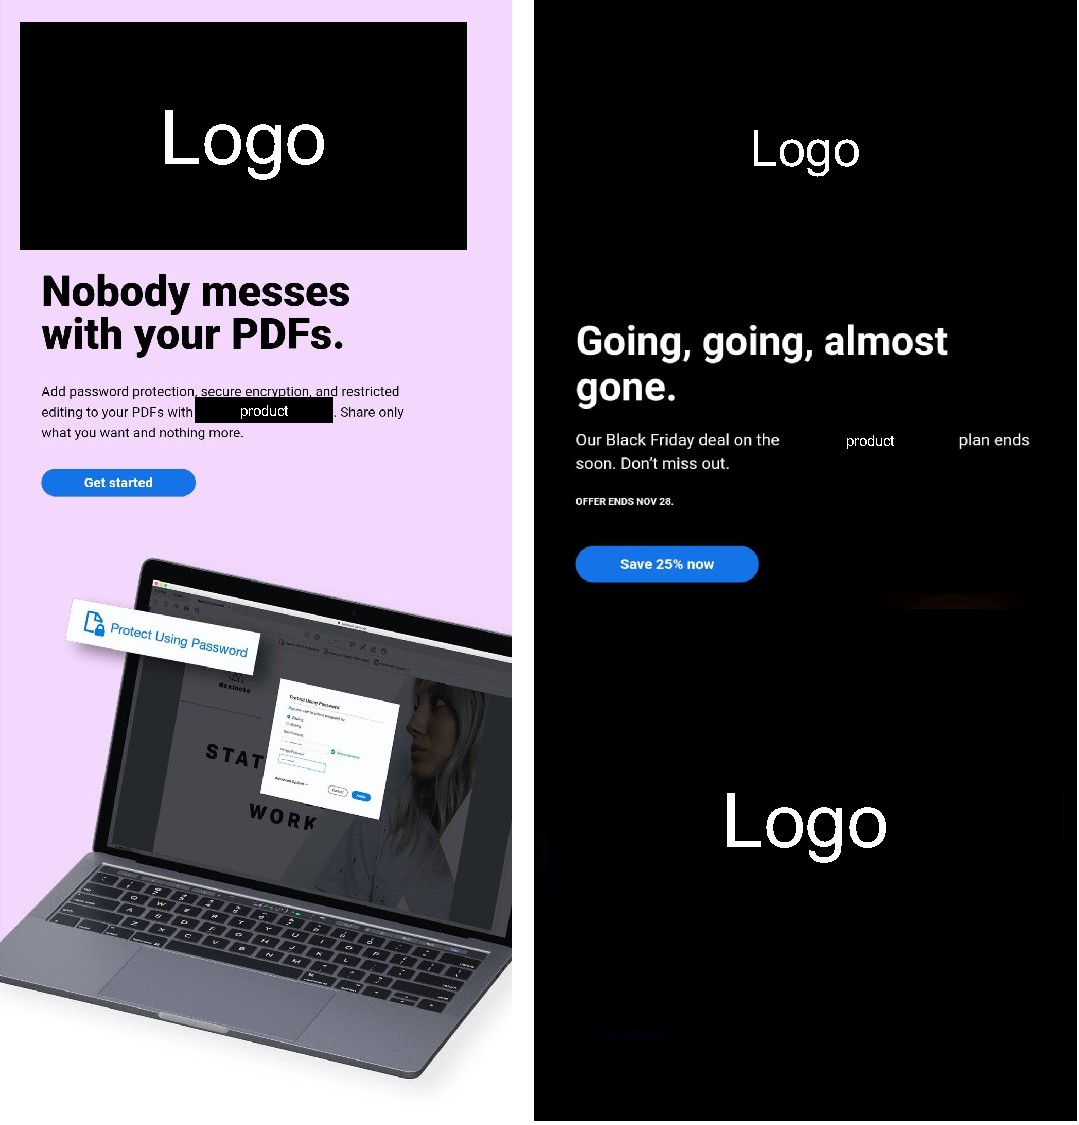
\includegraphics[width=0.7\textwidth]{images/email-ex-logo-redacted.pdf}
    \caption{The \companyName marketing emails used in the Email dataset look similar to the ones shown here.}
    \label{fig:figure-email-example}
\end{minipage}
\hfill
\begin{minipage}{\textwidth}\hspace{4pt}
\centering
\begin{adjustbox}{max width = 1.0\textwidth}\scriptsize
%\begin{tabular}{ll}\toprule[1.5pt]
\begin{tabularx}{0.7\textwidth}{XX}\toprule[1.5pt]
\textbf{Date Range} & April 1, 2022 to June 12, 2023 \\
\textbf{Number of Countries} & 225 \\
\textbf{Target Products} & Top Products used by millions of users\\ %Photoshop, Premiere Pro, Acrobat Professional, InDesign, XD, After Effects, Express, Creative Cloud, ... \\
\textbf{Customers Segmented on the basis of} & Type of use, user expertise, frequency of use, and others\\
\bottomrule[1.5pt]
\end{tabularx}
\end{adjustbox}
\caption{Details of the \companyName Marketing Email dataset used to evaluate behavior generalization capabilities of the LCBM
\label{table:email dataset}}
%\end{table*}
\end{minipage}
\end{figure}   


\subsection{Model}
\label{sec:model}
To understand both visual and textual contents, we follow a similar approach as was taken by recent models like BLIP, Llava, VideoLlama, and others \cite{liu2023visual,ge2023planting,li2023blip2,zhu2023minigpt}, we use visual encoders to encode visual knowledge and an LLM to encode text and world knowledge. Fig.~\ref{fig:lcbm-architecture} shows our architecture to encode visual content into the language space. We include video content by encoding video frames through EVA-CLIP \cite{sun2023eva} and Global Multi-Head Relation Aggregator (GMHRA) from Uniformer \cite{li2021uniformer}. GMHRA helps aggregate the information better across the time dimension. The combination of ViT and GMHRA gives us a good representation of the visual content. Next, to effectively leverage the LLM’s rich language representations, we use Q-Former from BLIP-2 \cite{li2023blip2} with an extra linear layer and additional query tokens to convert from visual tokens to language tokens. Further, similar to \cite{bhattacharyya-etal-2023-video}, we find that while encoding visual tokens is powerful, converting visual content to text adds to the downstream performance. Therefore, we include the BLIP caption for each scene along with the scene replay graph. 


We use the Llama-based Vicuna-13B LLM \cite{touvron2023llama,vicuna2023} as our base LLM. Similar to prior works \cite{liu2023visual,ge2023planting,li2023blip2,zhu2023minigpt}, we follow a two-stage training paradigm where in the first stage, we utilize the WebVid \cite{bain2021frozen}, COCO caption \cite{chen2015microsoft}, Visual Genome \cite{krishna2017dense}, CC3M \cite{sharma2018conceptual}, and CC12M \cite{changpinyo2021conceptual} datasets to align the visual encoder embeddings with LLM. In the second stage, we train the model with behavior instructions prepared by following the approach described in \S\ref{sec:behavior-instruction-tuning}. In summary, LCBM takes concatenated inputs of visual tokens, scene ASR, caption, scene behavior of replays, channel information, and video title and behavior metrics of views and a ratio of likes to views. Based on the instruction, we test LCBM's abilities on various tasks we cover in the next paragraphs.


%%%%%%%%%%%%%%%%%%%%%%%%%%%%%%%%%%%%%%%%%%%%%%%%%%%%%%%%%%%%%%%%%%%%%%
%%%%%%%%%%%%%%%%%%%%%%%%%%%%%%%%%%%%%%%%%%%%%%%%%%%%%%%%%%%%%%%%%%%%%%

\begin{center}
\begin{table*}[tbp]
\centering
\scriptsize
\begin{adjustbox}{width=\textwidth}\begin{tabular}{lcccccccccccc}\toprule[1.5pt]
\textbf{Model} & \textbf{\#Params} & \textbf{Training} & \multicolumn{2}{c}{\textbf{Past}} & \multicolumn{2}{c}{\textbf{Future}} & \multicolumn{4}{c}{\textbf{Random}} & \multicolumn{2}{c}{\textbf{All Masked}}\\
 &  & & & & & & \multicolumn{4}{c}{\textbf{Window Size}} & &\\\cmidrule{8-11}
 & & & & & & & \multicolumn{2}{c}{\textbf{5}} & \multicolumn{2}{c}{\textbf{7}}\\
 & & & \textbf{RMSE} & \textbf{Accuracy} & \textbf{RMSE} & \textbf{Accuracy} & \textbf{RMSE} & \textbf{Accuracy} & \textbf{RMSE} & \textbf{Accuracy} & \textbf{RMSE} & \textbf{Accuracy} \\ \hline
\textbf{LCBM} & \multirow{4}{*}{13B} & 3-BFT & \valbest{8.12} & \valbest{55.10} & \valgood{15.05} & 42.42 & \valgood{8.55} & \valgood{61.41} & \valgood{9.91} & \valgood{55.10} & - & -\\
\textbf{LCBM} & & 5-BFT & \valgood{11.53} & \valgood{52.06} & \valbest{12.02} & \valbest{53.06}  & \valbest{8.13} & \valbest{64.83} & \valbest{9.22} & \valbest{60.26} & \valbest{31.34} & \valbest{17.16}\\
\textbf{LCBM} & & 7-BFT & 16.17 & 35.61 & 15.14 & \valgood{44.11} & 9.02 & 59.22 & 10.47 & 53.84 & - & -\\
\textbf{LCBM} & & 11-BFT & 18.25 & 30.95 & \valgood{15.05} & 41.44 & 10.01 & 55.15 & 10.49 & 52.61& - & -\\ \hline
\textbf{GPT-4} & \multirow{2}{*}{$>$100B\footnotemark[2]} &  10-shot-ICL & 34.45 & 20.55 & 19.51 & 36.08 & 22.99 & 26.99 & 27.25 & 17.27 & 38.52 & 14.26\\
\textbf{GPT-4} & & 2-shot-ICL & 35.05 & 19.34 & 18.07 & 39.33 & 17.42 & 38.10 & 21.26 & 28.05 & 37.60 & 13.73 \\\hline
% GPT-4 & 0-shot & 81.50 & 12.36 & 246.87 & 25.88 & 165.59 & 23.60 & & \\\hline
\textbf{GPT-3.5} & \multirow{2}{*}{175B} & 3-shot-ICL & 34.10 & 19.06 & 24.71 & 27.14 & 24.52 & 24.81 & 26.30 & 18.74 & 38.77 & 13.47\\
\textbf{GPT-3.5} & &  2-shot-ICL & 33.36 & 18.02 & 26.44 & 25.42 & 23.35 & 25.35 & 24.68 & 21.24 & 37.16 & 13.39 \\\hline
% GPT-3.5 & 1-shot & 37.06 & 15.49 & 18.22 & 31.85 & 22.03 & 25.00 & 22.46 & 22.09\\\hline
% GPT-3.5 & 0-shot & 40.80 & 15.44 & 38.45 & 14.40 & 32.22 & 18.31 & & \\\hline
\textbf{Random} & - & - & 34.10 & 10.00 & 34.10 & 10.00 & 34.10 & 10.00 & 34.10 & 10.00 & 34.10 & 10.00\\\hline
\bottomrule[1.5pt]

\end{tabular}
\end{adjustbox}


\iffalse
    \begin{center}
    \begin{adjustbox}{max width=0.8\textwidth}\begin{tabular}{lccc}\toprule[1.5pt]
    \textbf{LLM} & \textbf{Training} & \multicolumn{2}{c}{\textbf{All Masked}}\\
     & & \textbf{RMSE} & \textbf{Accuracy} \\\hline
    \textbf{LCBM} & SFT & \valbest{31.34} & \valbest{17.16}\\\hline
    GPT-4 & 10-shot & 38.52 & 14.26\\
    GPT-4 & 2-shot & 37.60 & 13.73\\\hline
    GPT-3.5 & 3-shot & 38.77 & 13.47\\
    GPT-3.5 & 2-shot & 37.16 & 13.39\\\hline
    % GPT-3.5 & 1-shot & 37.99 & 5.75\\\hline
    Random & - & 34.10 & 10.00\\\hline
    \bottomrule[1.5pt]
    
    \end{tabular}
    \end{adjustbox}
    \end{center}
\fi
    
\caption{\textbf{Behavior Simulation.} Mean RMSE and accuracy scores for scene-by-scene predictions of video replay values. Replay values are the normalized replay scores of each scene as provided by YouTube. The normalized scores are considered to 2 decimal places and multiplied by hundred to convert the score to an integer score in the range 0-100. RMSE is calculated for each video in the test set and the mean is calculated for this score and reported. The model is said to classify correctly if the absolute error between the predicted and ground truth value is less than or equal to 5. The scores are calculated in four regimes: past, future, random, and all-masked. In the past (future) regimes, first (last) 5-20\% scenes are masked; in the random setting, 5-20\% scenes are masked randomly, and in all masked setting, everything is masked. LCBM was behavior-fine-tuned (BFT) with 3,5,7,11 context window masking strategy, while GPT was compared with an in-context learning (ICL) setting.  We note that behavior fine-tuned LCBM, while being at least 10x smaller than other models, performs the best. Best models are denoted in \valbest{green} and runner-ups in \valgood{blue}. \label{table:behavior-simulation-replay-values}}
\end{table*}
\end{center}






\subsection{Content Behavior Test Benchmark}
\label{sec:downstream tasks}
\label{sec:test benchmark}
We test the capabilities of large content-behavior models on predictive and descriptive abilities on content and behavior, as illustrated in Fig:~\ref{fig:figure-1-lcbm}. We design the following five tasks to test these capabilities: behavior simulation, content simulation, content understanding, behavior understanding, and behavior domain adaptation.
We cover each of these tasks next.


\begin{enumerate}[leftmargin=*]
    \item\textbf{Behavior Simulation.} We test simulation capability on four behaviors across two datasets: YouTube replay values, the ratio of YouTube likes to views, Twitter likes, and the number of views of the YouTube video. The common task amongst all of them is to predict the behavior given the content and content attributes like captions, scene-by-scene descriptions for videos, and sender characteristics like account and subscriber count and date of posting. The behavior to be predicted is masked and asked as a question to the LLM. Listings~\ref{listing:behavior-simulation-video-verbalization} and \ref{listing-twitter-behavior-simulation} lists the verbalization pattern for this task. For replay value prediction, we test the masked behavior in three settings: \textit{Masked Past} (all replay values of the first 5-20\% scenes are masked), \textit{Masked Future} (all replay values of last 5-20\% scenes are masked), and \textit{Random Masks} (random masking of replay values for 5-20\% scenes).

    
    % \item Image Content: Given the image content, ground truth caption, objects present in the image, object locations, image visual complexity, and date of publication, predict the number of downloads and number of licenses purchased. The template for this is presented in Listing~\ref{listing:behavior-simulation-image-verbalization}.

    \item\textbf{Content Simulation.} Here, the task is to predict content given receiver behavior (Listings~\ref{listing-video-content-simulation}, \ref{table:content-simulation-twitter}). For YouTube, given the video content in terms of scene-by-scene descriptions with the content of one group of five consecutive scenes content being masked, behavior values of all scenes, and channel information, the task is to choose the masked scene speech from a list of 25 options, chosen randomly from the entire test set. For YouTube, we chose to model this task as a discriminative task instead of a generative one since videos are generally long, and there could be multiple possible contents for a given behavior, whereas the ground truth is available only for one specific characterization of the content for a given behavior. For Twitter, we model this task as content generation. The Listing~\ref{listing-twitter-content-simulation} presents the format for this task.
    
    \item\textbf{Behavior Understanding.} The goal of this task is to check if the model can reason about observed or unobserved receiver behavior. For this task, we could ask the model to explain any behaviors given the content. However, only the YouTube receiver comments have ground truth available with the video. Without ground truth, we found that other behaviors, such as replay values, likes, and views, are difficult to explain by non-experts. Therefore, we ask the model to simulate the sentiment of the receivers' comments and describe its reasoning. To evaluate, we asked six annotators to annotate the reasons provided by the model on a scale of 0-5, with 0 implying the LLMs provided no sentiment or reasoning and 5 implying perfect reasoning. The annotators were free to rate the LLMs as they seemed fit. The annotators were asked to review the video content and the comments to help them evaluate the reasons. We average the ratings of three annotators to get an average rating for every video. Similarly, to review the sentiment correctness, we asked the annotators to judge the predicted sentiment rating with respect to user comments.
    
    \item\textbf{Content Understanding.} To check if a model trained on both content and behavior tokens does not forget its original content understanding capabilities, we test the content understanding tasks on YouTube videos, following \cite{bhattacharyya-etal-2023-video}. They use the following tasks for video-understanding: topic, emotion, persuasion, and action-reason classification. For topic, emotion, and action-reason classification tasks, they use the advertisements dataset by \cite{hussain2017automatic}, which contains 3,477 video advertisements and the corresponding annotations for emotion and topic tags and action-reason statements for each video. There are a total of 38 topics and 30 unique emotion tags per video. Further, we have 5 action-reason statements for each video for the action-reason generation task. For our experiment, we use the subset of 1,785 public videos.  Following \cite{bhattacharyya-etal-2023-video}, for the topic and emotion classification task, we evaluate our pipeline using top-1 accuracy as the evaluation metric. Further, we evaluate emotion classification on clubbed emotion labels as well. For action and reason prediction, we evaluate our accuracy on the action and reason retrieval tasks where 29 random options along with 1 ground truth are provided to the model to find which one is the ground truth.
    In the persuasion strategy classification, we use the 1002 persuasion strategy videos and corresponding labels released by \cite{bhattacharyya-etal-2023-video}. Given the video, the model has to predict which persuasion strategy the video conveys. Persuasion strategy classification could be an important task for evaluating LCBM since the concept of persuasion in psychology views human communication as the means to change the receiver's beliefs and actions (\textit{i.e.}, to persuade) \cite{kumar2023persuasion}, and understanding the different strategies present in communication may help understand human behavior better. We evaluate the top-1 accuracy of the model on this task.
    
    \item\textbf{Behavior Domain Adaptation.} In the past work, we have observed strong generalization capabilities from LLMs \cite{openai2023gpt4,ouyang2022training,raffel2020exploring}. While training on next token prediction, LLMs show generalization across tasks, including question answering, natural language inference, and sentiment analysis. Given this, the natural question is, does LCBM, too, show this kind of generalization, where a model trained on one kind of behavior, can show performance on another behavior? To understand this, we test the model on a different dataset and task than what it was originally trained for. We do this over three datasets, LVU \cite{wu2021towards}, \companyName Email Marketing\footnotemark[6], and generalization between Twitter and YouTube likes.
    
    \begin{itemize}
        \item\textbf{LVU Benchmark.} Wu \textit{et al.} \cite{wu2021towards} released a benchmark for long video understanding with over 1000 hours of video. In the benchmark, they have two behavior related tasks: ratio of likes to likes+dislikes and view prediction. YouTube has discontinued the dislike count, therefore, our corpus does not contain the dislike count. We use the LVU test benchmark to check if a model trained on other available behaviors (views, likes, and replay graphs) is able to predict the like ratio.
        
        \item\textbf{\companyName Email Marketing.} In this task, we ask the model to predict the click-through rate for a given target segment of an email, given the email content, subject, and verbalized descriptions of the images in the email. We use the emails sent by \companyName marketing team to its subscribers. The emails were sent from April 1, 2022 to June 12, 2023 and covered many of the premiere products %of Adobe, including Photoshop, Premiere Pro, Acrobat, and Indesign. 
        The emails were sent to many customer segments (as defined by the marketing team) across 225 countries (Fig.~\ref{table:email dataset}). Listing~\ref{listing-email-content-behavior-simulation} lists the verbalization format to verbalize emails to input to the LCBM. 
    \end{itemize}
\end{enumerate}







\begin{center}
\begin{table*}[tbp]
\begin{center}
\begin{adjustbox}{max width=\textwidth}\footnotesize\begin{tabular}{lcccccc}\toprule[1.5pt]
\textbf{Model} & \textbf{\#Params} & \textbf{Training type} & \textbf{Training} & \textbf{RMSE} & \textbf{R$^2$} & \textbf{Accuracy} \\\hline
%\multicolumn{3}{c}{\textbf{Past}} & \multicolumn{3}{c}{\textbf{Future}} & \multicolumn{6}{c}{\textbf{Random}}\\
% & & & & & & & & \multicolumn{6}{c}{\textbf{Window Size}}\\\cmidrule{9-14}
% & & & & & & & & \multicolumn{3}{c}{\textbf{5}} & \multicolumn{3}{c}{\textbf{7}} \\
% & & \textbf{RMSE} & \textbf{R$^2$} & \textbf{Accuracy} \\\hline% & \textbf{RMSE} & \textbf{R$^2$} & \textbf{Accuracy} & \textbf{RMS}E & \textbf{R$^2$} & \textbf{Accuracy} & \textbf{RMSE} & \textbf{R$^2$} & \textbf{Accuracy} \\\hline
\textbf{LCBM}& \multirow{4}{*}{13B} & BFT & Replay values 3-masked & \valbest{1.31} & \valbest{0.87} & \valgood{15.89} \\
%\valgood{1.36} & \valbest{0.86} & \valgood{14.04} & 1.45 & \valgood{0.84} & \valgood{15.30} & \valbest{1.31} & \valbest{0.87} & \valgood{15.89} & \valgood{1.39} & \valgood{0.86} & \valgood{15.60}\\ 
\textbf{LCBM} & & BFT & Replay values 5-masked & \valgood{1.48} & \valgood{0.82} & \valbest{19.93}\\
%1.48 & 0.82 & \valbest{19.93} & \valgood{1.44} & \valgood{0.84} & \valbest{18.69} & \valgood{1.38} & \valgood{0.85} & \valbest{18.13} & 1.47 & 0.83 & \valbest{19.02}\\
\textbf{LCBM} & & BFT & Replay values 7-masked & 1.71 & 0.78 & 15.20\\
%1.53 & \valgood{0.82} & 11.21 & 1.71 & 0.78 & 15.20 & 1.61 & 0.81 & 12.38 & \valbest{1.36} & \valbest{0.87} & 13.94\\
\textbf{LCBM} & & BFT & Replay values 11-masked & 1.55 & \valgood{0.82} & 13.94\\\hline
%\valbest{1.35} & \valbest{0.86} & 12.38 & \valbest{1.43} & \valbest{0.85} & 13.26 & 1.55 & 0.82 & 13.94 & 1.51 & 0.83 & 13.74 \\ \hline
% GPT-4 & 10-shot & 1.97 & 0.76 & 1.69 & 3.46 & 0.11 & 7.66 & 4.00 & 0.07 & 2.59 & 2.53 & 0.62 & 3.27 & 2.06 & 0.75 & 0.62\\\hline
\textbf{GPT-4} &\multirow{2}{*}{$>$100B\footnotemark[2]} & ICL & 10-shot & 3.50 & -0.01 & 7.84\\
%& 3.61 & 0.09 & 5.66 & 3.50 & -0.01 & 7.84 & 5.75 & -1.20 & 5.37 & 3.88 & -0.01 & 7.69\\
% GPT-4 & 2-shot & 5.29 & -1.26 & 3.06 & 5.73 & -1.46 & 4.86 & 16.12 & -19.38 & 3.86 & 3.41 & 0.16 & 4.89 & 11.49 & -9.10 & 4.66\\\hline
\textbf{GPT-4}& & ICL & 2-shot & 3.58 & -0.03 & 5.39\\\hline
%5.97 & -2.22 & 3.91 & 5.78 & -1.77 & 4.95 & 16.95 & -24.00 & 4.27 & 3.58 & -0.03 & 5.39\\\hline
% GPT-4 & 0-shot & 3.51 & -0.05 & 5.26 & 5.82 & -1.84 & 5.48 & 4.72 & -0.90 & 4.89 & & &\\\hline
% GPT-3.5 & 3-shot & 26.06 & -55.92 & 0.10 & 73.11 & -473.69 & 0.60 & 25.78 & -34.81 & 0.40 & 18.49 & -15.13 & 0.01 & 4.76 & -3.88 & 4.05\\\hline
\textbf{GPT-3.5}& \multirow{2}{*}{175B} & ICL & 3-shot & 64.40 & -256.96 & 2.48\\
%64.58 & -385.57 & 0.62 & 77.13 & -583.33 & 0.67 & 64.40 & -256.96 & 2.48 & 70.03 & -251.73 & 0.0\\
% GPT-3.5 & 2-shot & 34.55 & -105.97 & 0.40 & 71.36 & -362.56 & 0.01 & 27.12 & -92.21 & 0.00 & 15.98 & -14.17 & 0.00 & 4.76 & -3.88 & 4.05\\\hline
\textbf{GPT-3.5} & & ICL & 2-shot & 64.88 & -375.83 & 1.27\\\hline
%64.88 & -375.83 & 1.27 & 78.12 & -487.44 & 0.12 & 76.52 & -839.52 & 0.00 & 67.39 & -303.53 & 0.00\\\hline
% GPT-3.5 & 1-shot & 13.07 & -15.74 & 0.09 & 17.86 & -21.58 & 0.60 & 13.69 & -9.33 & 3.53 & 1.99 & 0.60 & 0.91 & 4.76 & -3.88 & 4.05\\\hline
% GPT-3.5 & 0-shot & 4.64 & -0.52 & 3.87 & 5.45 & -1.28 & 2.36 & 3.87 & -0.29 & 1.87 & & & \\\hline
\textbf{Random} & - & - & - & 4.67 & 0 & 3.94 \\\hline
%& 4.67 & 0 & 3.94 & 4.67 & 0 & 3.94 & 4.67 & 0 & 3.94\\\hline
\bottomrule[1.5pt]
\end{tabular}
\end{adjustbox}
\end{center}
\caption{\textbf{Behavior Simulation.} RMSE, R$^2$, and accuracy scores for like/view ratio prediction task. To calculate accuracy, the model is said to classify correctly if the absolute error between the predicted and ground truth likes/views is less than or equal to 10\%. BFT denotes behavior fine-tuning, and ICL stands for in-context learning. Replay values $k$-masked means a model which is trained by masking $k$ consecutive values of the replay graph while doing BFT. We note that LCBM while being at least 10x smaller than the other models, performs the best. The best results over four runs are reported for all models. Best models are denoted in \valbest{green} and runner-ups in \valgood{blue}. \label{table:behavior-simulation-like-simulation}}
\end{table*}
\end{center}
\footnotetext[2]{The exact size of GPT-4 is unknown.}





%%%%%%%%%%%%%%%%%%%%%%%%%%%%%%%%%%%%%%%%%%%%%%%%%%%%%%%%%%%%%%%%%%%%%%
%%%%%%%%%%%%%%%%%%%%%%%%%%%%%%%%%%%%%%%%%%%%%%%%%%%%%%%%%%%%%%%%%%%%%%

\subsection{Behavior Instruction Fine-Tuning (BFT)}
\label{sec:behavior-instruction-tuning}
To teach an LLM the behavior modality over multimodal content, we convert both the visual tokens and behavior modality in the text format and instruction fine-tune the LLM end to end. This follows a two-stage approach: first, we teach the LLM the visual modality (\S\ref{sec:model}), and next, we teach the LLM the behavior modality. We call the latter ``Behavior Instruction Fine-Tuning (BFT)'' inspired by instruction fine-tuning (IFT) and its variants like visual instruction tuning \cite{liu2023visual}.


%We use the instruction fine-tuned LLM, VideoChat, to teach it the behavior modality. VideoChat is a vision language model (VLM) that combines video and image foundation models and large language models (LLMs) through a learnable neural interface. VideoChat follows a two-stage training: one where it aligns a video- and image-encoder embedding space with the text encoder embedding space and a second step where it instruction-tunes the LLM using a video- and image-language instruction dataset. This results in a VLM, which now understands spatiotemporal perception and reasoning on vision and language data. We base our content-behavior model on VideoChat. We further instruction-fine-tune VideoChat on content aligned behavior data to teach it the behavior modality. We expand on that next.


We prepare the content-behavior instruction datasets as explained next.

\textbf{Teaching behavior in the forward direction} (predict behavior given content): In this instruction tuning task, we teach the model to predict behavior given the message sent by the communicator. Essentially, this teaches the model to predict behavior in the forward direction (as in Fig.~\ref{fig:factors-of-communication-chapter-lcbm}). Concretely, we include the following information as part of verbalization - image and video embedding converted to the text space (using EvaCLiP \cite{sun2023eva}), scene-by-scene verbalization covering automatic speech recognition, scene captions, video/post caption and description, receiver behavior covering replay rates, views, and likes, and communicator information covering account name and follower count. The verbalisation pattern for this task is the same as given in the Listing~\ref{listing:behavior-simulation-video-verbalization}.
%We observed that VideoChat's hallucinations increase substantially when the video length increases. Therefore, we choose videos with a length between 10 and 100 seconds.

\textbf{Teaching behavior in the reverse direction} (predict content given behavior): This task teaches the model to learn about behavior in the reverse direction (Fig.~\ref{fig:factors-of-communication-chapter-lcbm}). Here, the model learns to simulate content given behavior. The instruction for this task is given in Listing~\ref{listing-content-simulation-verbalization}.


% 2. Adobe Stock Images: For an image $I$ from Adobe Stock, we have the following receiver behavior: downloads and all-time licenses. Further, we verbalize images by including objects detected using recognize anything model \cite{zhang2023recognize,huang2023tag2text}, object positions using segment anything model \cite{liu2023grounding,kirillov2023segany}, visual complexity using \cite{feng2023ic9600}, ground truth user-provided image captions, and date of posting the image online\footnote{Notably, we do not have information about the receiver in either YouTube or Adobe Stock. Correspondingly, we have average receiver behavior for both datasets.}. 



Using the prepared content and behavior instruction datasets consisting of pairs of content and behavior tokens, we treat the content tokens ($\mathbf{X}_C$) as input and behavior tokens ($\mathbf{X}_B, x_i\in\mathbf{X}_B$) as output of the language model. We then perform instruction-tuning of the LLM on the prediction tokens, using its original auto-regressive training objective. Specifically, for a sequence of length L, we compute the probability of generating target answers ($\mathbf{X}_B$) by:
\begin{equation}
    p(\mathbf{X}_B | \mathbf{X}_C) = \prod_{i=1}^{L} p_{\theta}(x_i | \mathbf{X}_C, \mathbf{X}_{B, <i})
\end{equation}
For the behavior instruction tuning, we keep the visual encoder weights frozen and continue to update the pre-trained weights of the LLM in LCBM. 




%%%%%%%%%%%%%%%%%%%%%%%%%%%%%%%%%%%%%%
%%%%%%%%%%%%%%%%%%%%%%%%%%%%%%%%%%%%%%


\begin{center}
\begin{table}[tbp]
\begin{minipage}{\linewidth}
\begin{center}
\begin{adjustbox}{max width=\columnwidth}\footnotesize\begin{tabular}{lcc}\toprule[1.5pt]
\textbf{Model} & \textbf{\#Params} & \textbf{Accuracy} \\\hline
Vicuna & 13B & 19.30\% \\
LCBM & 13B& \valbest{48.68\%} \\
GPT-3.5 & 175B & \valgood{34.98\%}  \\
Random & - & 4\%\\
\bottomrule[1.5pt]
\end{tabular}
\end{adjustbox}
\end{center}
\caption{\textbf{Content Simulation.} In this task, the models have to choose the speech segment from a list of 25 options given the video description, non-masked scenes. and replay behavior. We see that despite being similar to masked language modeling (which is a content-only task), LCBM performs better than both Vicuna and GPT-3.5. Best models are denoted in \valbest{green} and runner-ups in \valgood{blue}. \label{table:content-simulation}}
\end{minipage}
\hspace{4pt}
\begin{minipage}{\linewidth}
\begin{center}
\begin{adjustbox}{max width=1.0\columnwidth}
\scriptsize\begin{tabular}{lccc}\toprule[1.5pt]
\textbf{Model} & \textbf{\#Params} & \textbf{Sentiment Accuracy} & \textbf{Reasoning Score} \\\hline
\textbf{Vicuna} & 13B & \valgood{65.66\%} & \valgood{2.23} \\
\textbf{LCBM} & 13B & \valbest{72.73\%} & \valbest{4.00} \\
\textbf{GPT-3.5} & 175B & 61.62\% & 1.67 \\
\bottomrule[1.5pt]
\end{tabular}
\end{adjustbox}
\end{center}
\caption{\textbf{Behavior Understanding.} In this task, the models have to simulate the sentiment of comments that a video would get by looking at only the video. Further, they also have to explain the reason for such sentiment. The responses were annotated by humans on a scale of 0-5 for the reason, with 0 being no response provided and 5 being the response matches exactly with the (ground truth) comments received on the video. Best models are denoted in \valbest{green} and runner-ups in \valgood{blue}. \label{table:behavior-understanding}}
\end{minipage}
\end{table}
\end{center}




\begin{table*}[!tp]
\centering
\scriptsize
\begin{minipage}{\linewidth}
\centering
\begin{adjustbox}{max width = 1.0\textwidth}
\begin{tabular}{llcccccccc}\toprule[1.5pt]
\multirow{2}{*}{\textbf{Training}} & \multirow{2}{*}{\textbf{Model}} & \textbf{\#Params} &\textbf{Topic} &\multicolumn{2}{c}{\textbf{Emotion}} & \textbf{Persuasion} &\textbf{Action} &\textbf{Reason}\\\cmidrule{4-5}
& & & \textbf{All labels} & \textbf{Clubbed} \\ \midrule[0.5pt]
\textbf{Random} & \textbf{Random} &- & 2.63 & 3.37 & 14.3 & 8.37 & 3.34 & 3.34 \\\hline
% Fine-Tuned & VideoMAE \cite{tong2022videomae} & 24.72 & 29.72 & \valgood{85.55}  & 11.17  & - & - \\
% & \citet{hussain2017automatic} & 35.1 & 32.8 & -  & - & - & 48.45 \\
% \ & Intern-Video \cite{wang2022internvideo} & 57.47 & \valbest{36.08} & \valbest{86.59} & 5.47 & 6.8 & 7.1 \\\hline
\textbf{Zero-shot} & \textbf{GPT-3.5} & 175B & \valbest{51.6} & \valbest{11.68} & \valbest{79.69} & \valbest{35.02} & \valbest{66.27} & \valbest{59.59} \\
% Zero-shot & GPT-3.5 Generated Story + Flan-t5-xxl Classifier & \valgood{60.5} & 10.8 & 79.10 &  \valgood{33.41} &  \valbest{79.22} & \valbest{81.72} \\
% & GPT-3.5 Generated Story + Vicuna Classifier & 22.92 & 10.8 & 67.35 & 29.6 & 21.39 & 20.89 \\
% & Vicuna Generated Story + GPT-3.5 Classifier & 46.7 & 5.9 & 80.33 & 27.54 & 61.88 & 55.44 \\
% & Vicuna Generated Story + Flan-t5-xxl Classifier & 57.38 & 9.8 & 76.60 & 30.11 & \valgood{77.38} & \valgood{80.66}  \\
& \textbf{Vicuna} & 13B & 11.75 & \valgood{10.5} & \valgood{68.13} & 26.59 & 20.72 & 21.00  \\
& \makecell[l]{\textbf{VideoChat}\\\cite{li2023videochat}} & 13B & 9.07 & 3.09 & 5.1 &  10.28 & - & - \\
& \textbf{LCBM} & 13B & \valgood{42.17} & 7.08 & 58.83 & \valgood{32.83} & \valgood{39.55} & \valgood{27.91}  \\\hline
% & Content-Behavior instruction fine-tuned VideoChat model + Flan-t5-xxl classifier & 58.38 & 8.52 & 78.94 & 26.22 &  &   \\\hline
\bottomrule[1.5pt]

\end{tabular}
\end{adjustbox}
\caption{\textbf{Content Understanding.} Comparison of several models, including behavior instruction tuned models before and after BFT. We compare the models across topic, emotion, and persuasion strategy detection tasks as per the framework given by \cite{bhattacharyya-etal-2023-video}. We see that our model outperforms similarly sized models (Vicuna, VideoChat) in most tasks. Best models are denoted in \valbest{green} and runner-ups in \valgood{blue}.\label{tab:content-understanding}}\end{minipage}
\end{table*}



%%%%%%%%%%%%%%%%%%%%%%%%%%%%%%%%%%%%%%
%%%%%%%%%%%%%%%%%%%%%%%%%%%%%%%%%%%%%%
\subsection{Results and Discussion}
\label{sec:results}
Here, we discuss the results for the five tasks we discuss in Section~\ref{sec:test benchmark}, namely, behavior simulation, content simulation, behavior understanding, content understanding, and behavior domain adaptation. We compare the behavior fine-tuned model discussed in \S\ref{sec:behavior-instruction-tuning} with state-of-the-art content-only models like GPT-3.5, GPT-4, and Vicuna-13B. This allows us to compare how much including behavior tokens in the training of an LLM helps in improving the LLM's understanding of behavior and joint content and behavior spaces while retaining its understanding of the content space. 

The results for the five tasks are presented in Tables~\ref{table:behavior-simulation-replay-values}, \ref{table:behavior-simulation-like-simulation}, \ref{table:content-simulation}, \ref{table:behavior-understanding}, \ref{tab:content-understanding}, \ref{table:behavior-domain-adaptation}, \ref{table:behavior-simulation-like-simulation-twitter}, and \ref{table:content-simulation-twitter}. We note a few general trends. LCBM, while being 10x smaller than GPT-3.5 and 4, performs better than them on all behavior-related tasks. Further, we see that there is no significant difference between 10-shot and 2-shot GPT-4 or between GPT-3.5 and GPT-4, indicating that unlike other tasks, it is harder to achieve good performance through in-context-learning on the behavior modality. It can be observed that often GPT-3.5 and 4 achieve performance comparable to (or worse than) random baselines. Interestingly, the performance of GPTs on the content simulation task is also substantially behind LCBM. The way we formulate the content simulation task (Listing~\ref{listing-video-content-simulation}), it can be seen that a substantial performance could be achieved by strong content knowledge, and behavior brings in little variance. We still see a substantial performance gap between the two models. All of this indicates that large models like GPT-3.5 and 4 are not trained on behavior tokens. 


For the content understanding tasks (Table~\ref{tab:content-understanding}), predictably GPT-3.5, being the largest model, achieves the best results. However, we see that BFT helps the LLM to learn most content understanding tasks better than the base LLM. LCBM gets better results than both Vicuna and VideoChat. This indicates that behavior modality might carry additional information about the content, which might help an LLM understand content better \cite{khurana-etal-2023-synthesizing,klerke-etal-2016-improving,plank2016keystroke}. 
Next, we see that LCBM also shows signs of domain adaptation in the behavior modality. We see that on five tasks: comment sentiment prediction, comment sentiment reasoning (Table~\ref{table:behavior-understanding}), email behavior simulation (Table~\ref{table:behavior-domain-adaptation}), and Twitter behavior (Table~\ref{table:behavior-simulation-like-simulation-twitter}) and content simulation (Table~\ref{table:content-simulation-twitter}). We note that if the LCBM is trained on only email behavior simulation samples, it underperforms the model trained on both YouTube data and a few samples to make the model learn email format. Similarly, LCBM trained on both Twitter and YouTube performs better than the one just trained on Twitter, showing performance improvement by domain adaptation. Finally, Figs.~\ref{fig:comment-explains},\ref{fig:replay-explains} show a few samples where we query LCBM to explain replay and comment behavior and compare it with human explanations. We see that LCBM while verbose, can explain behavior well.

\begin{figure*}[!t]
    \centering
    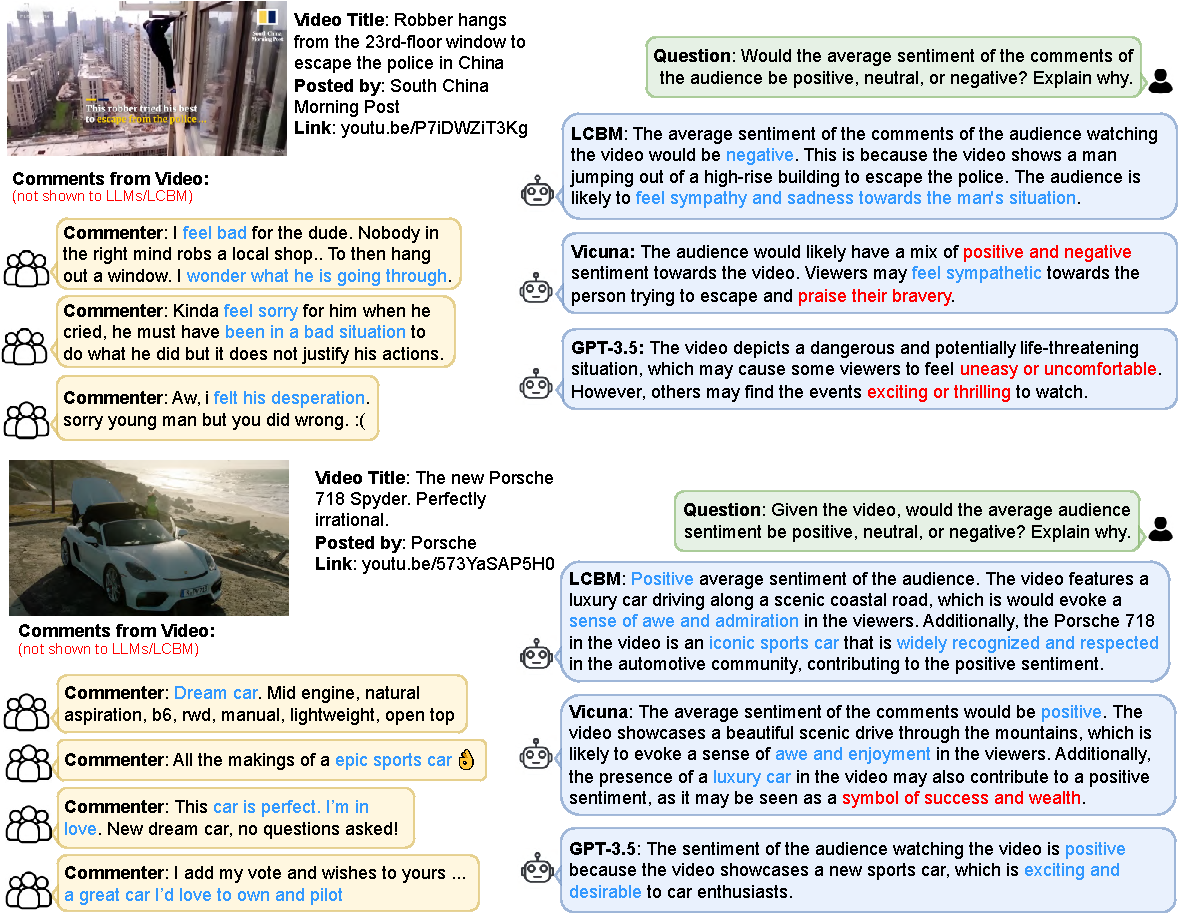
\includegraphics[width=\textwidth]{images/comment-explains-compressed.pdf}
    \caption{A few examples showing LCBM's ability to understand and explain human behavior of audience sentiment. We also compare it against other models like Vicuna and GPT-3.5. \label{fig:comment-explains}}
\end{figure*}


\begin{figure*}[!t]
    \centering
    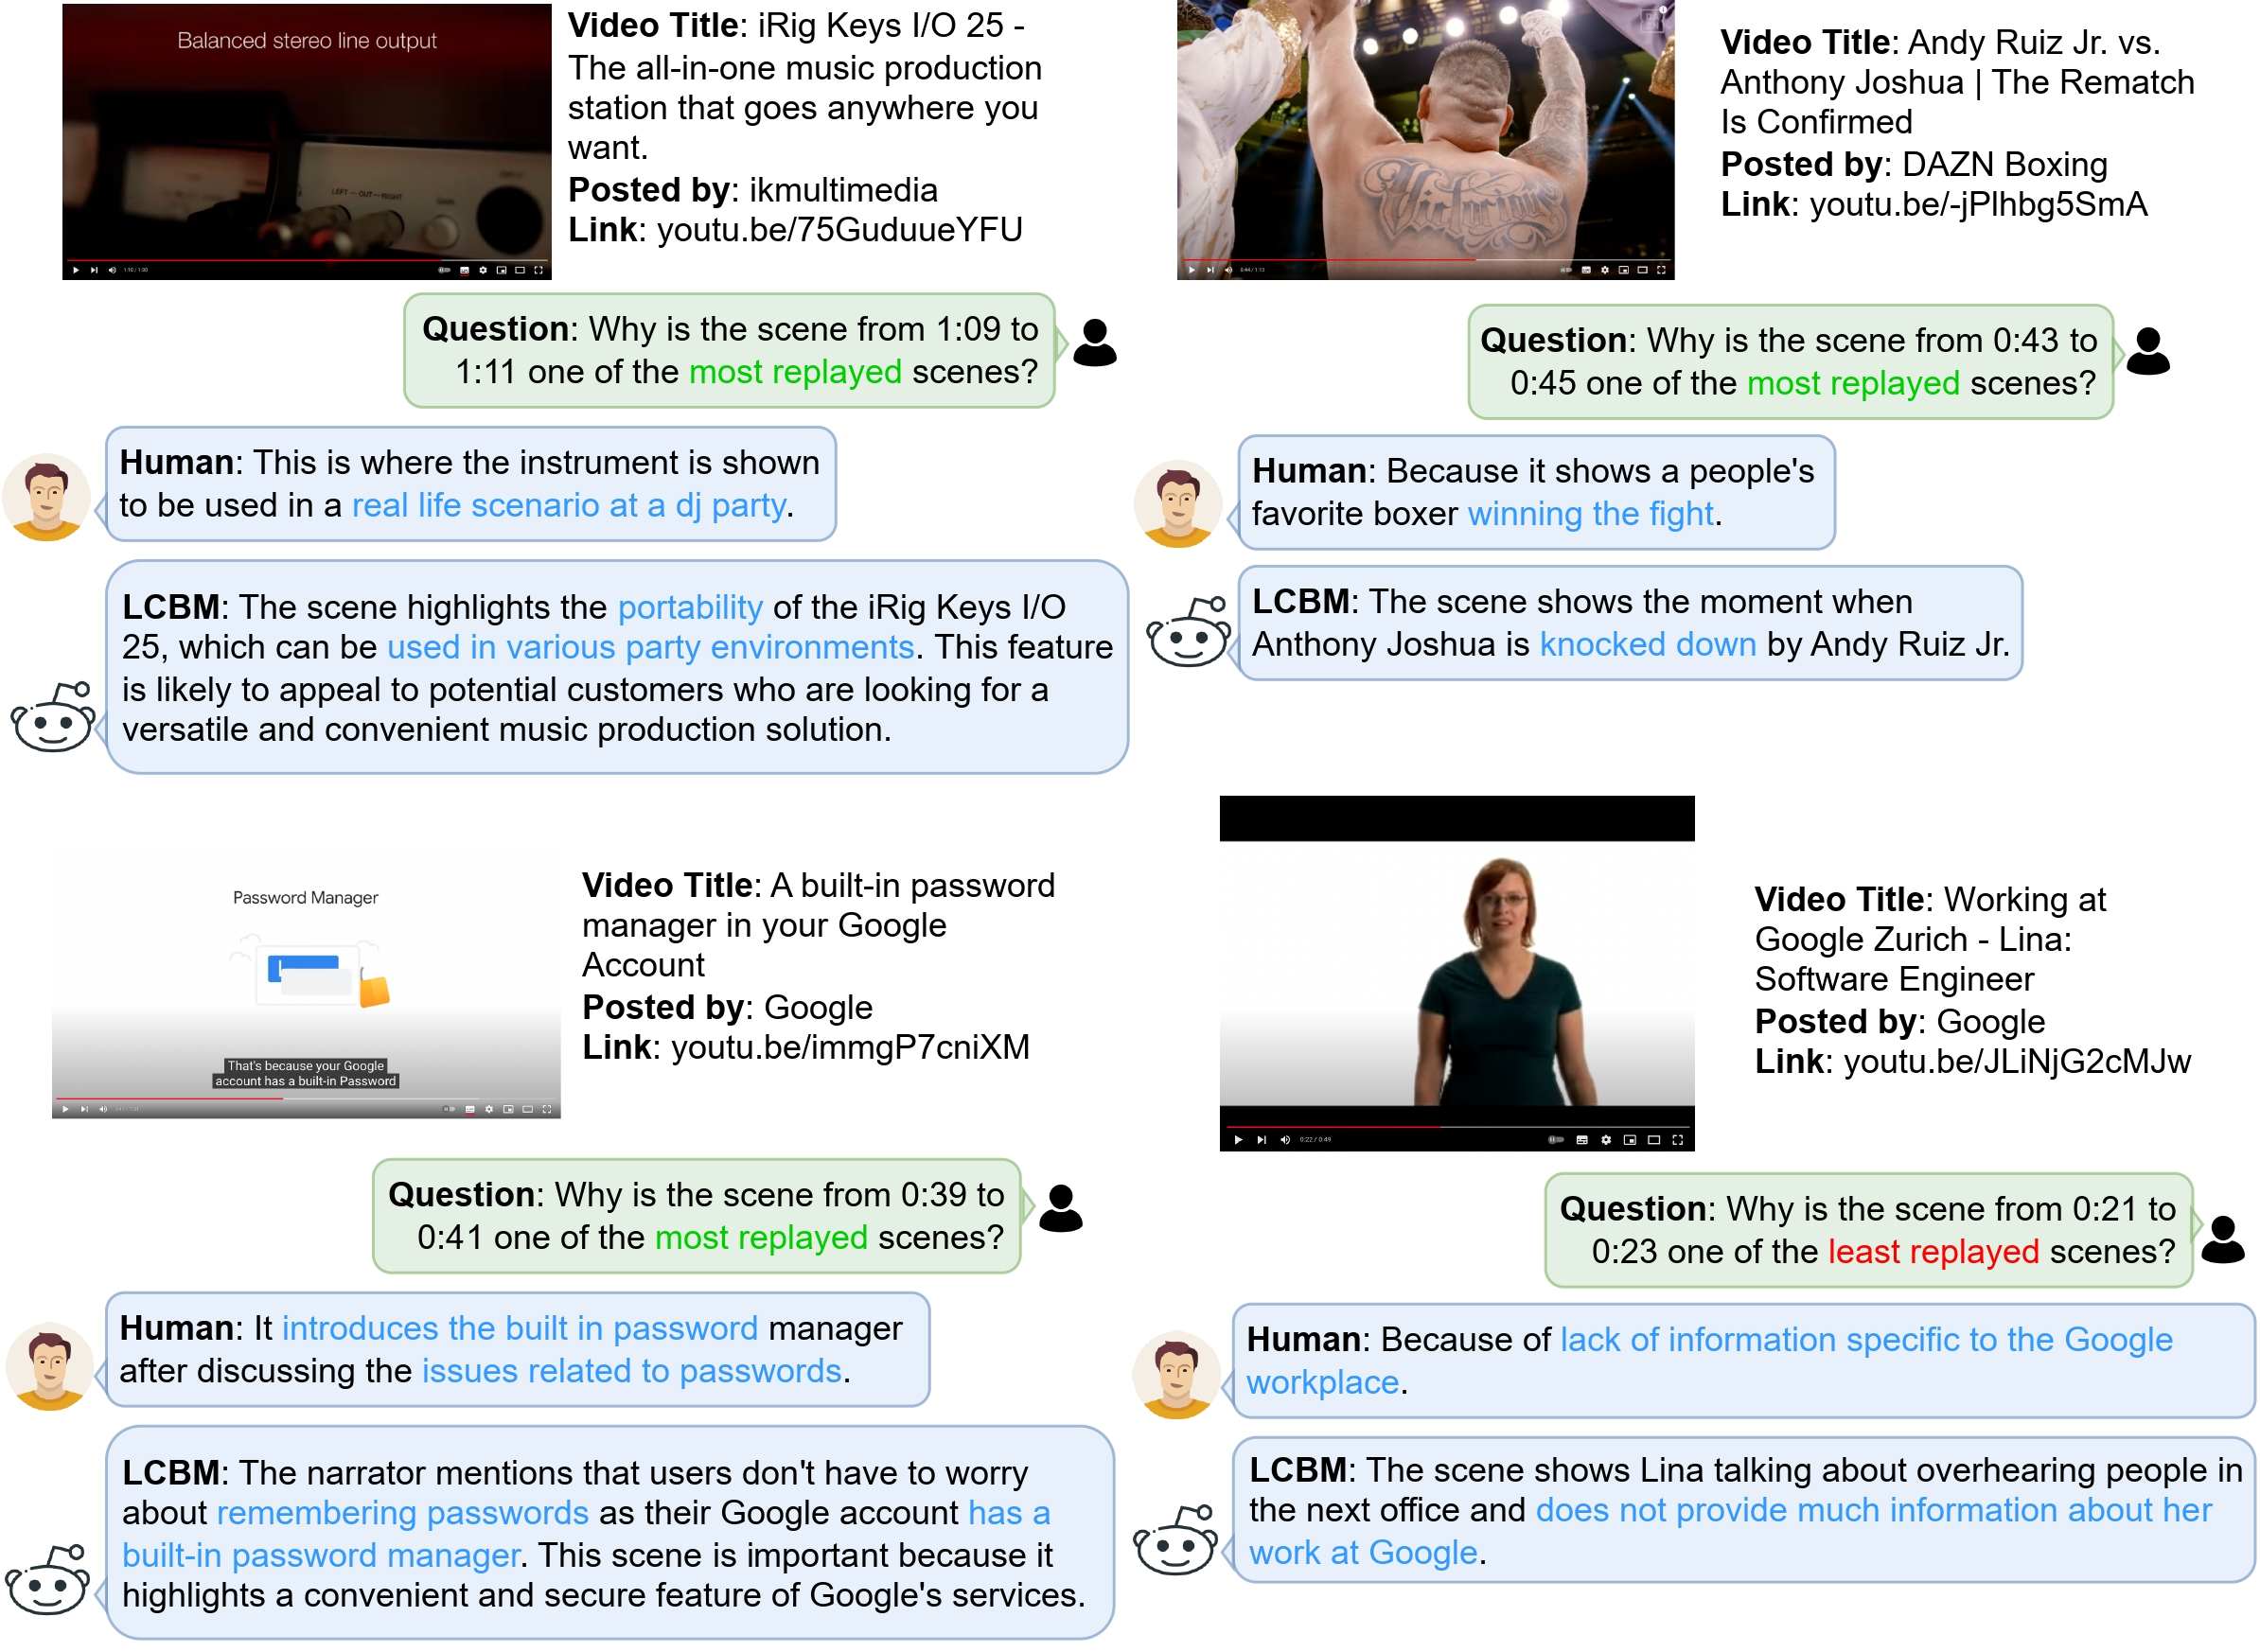
\includegraphics[width=\textwidth]{images/replay-explains.jpeg}
    \caption{A few examples showing LCBM's ability to understand and explain human behavior of scene replayability. We compare it against human-provided explanations of the same.    \label{fig:replay-explains}}
\end{figure*}



% \begin{center}
% \begin{table}[tbp]
% \begin{center}
% \begin{adjustbox}{max width=1.0\columnwidth}\begin{tabular}{|c|c|c|c|c|c|}
% \hline
% LLM & Task & Past & Future & \multicolumn{2}{|c|}{Random} \\
% \hline
%  & &  &  & \multicolumn{2}{|c|}{Window Size} \\
% \hline
%  & & & & 5 & 7 \\
% \hline
% Vicuna & 3 secs & 1.0 & 0.94 & 0.96 & 0.96 \\
% \hline
% Vicuna & 5 secs & 0.95 & 0.96 & 0.95 & 0.97 \\
% \hline
% Vicuna & 7 secs & 0.90 & 0.96 & 0.97 & 0.94 \\
% \hline
% Vicuna & 11 secs & 0.95 & 0.96 & 0.94 & 0.95 \\ \hline

% GPT-3.5 & few-shot & & & &  \\\hline
% GPT-4 & few-shot  & & & & \\\hline
% \end{tabular}\end{adjustbox}
% \end{center}
% \caption{Behavior-Simulation: Comparison on generation metrics. Best models are denoted in \valbest{green} and runner-ups in \valgood{blue}.}
% \end{table}
% \end{center}


% \begin{center}
% \begin{table*}[tbp]
% \begin{center}
% \begin{adjustbox}{max width=2.0\columnwidth}\begin{tabular}{|c|c|c|c|c|c|c|c|c|c|c|c|c|}\hline
% LLM & Training & \multicolumn{2}{|c|}{Past} & \multicolumn{2}{|c|}{Future} & \multicolumn{4}{|c|}{Random} & \multicolumn{2}{|c|}{All Masked} \\\hline
%  & &  &  &  & & \multicolumn{4}{|c|}{Window Size} & & \\\hline 
%  & & & & & & \multicolumn{2}{|c|}{5} & \multicolumn{2}{|c|}{7} & & \\ \hline
%  & & RMSE & Accuracy & RMSE & Accuracy & RMSE & Accuracy & RMSE & Accuracy & RMSE & Accuracy\\ \hline
% Vicuna & 3 & \valbest{7023518.62} & 4.00 & 11435377.05 & 3.70 & 10258208.91 & \valbest{4.78} & 11003562.06 & 7.41 & &\\ \hline
% Vicuna & 5 & 7879834.78 & \valbest{4.19} & 7938421.01 & \valbest{4.58} & \valgood{7145507.29} & \valgood{4.00} & 7112106.52 & 7.12 & &\\\hline
% Vicuna & 7 & 7136886.01 & 2.53 & \valbest{6955264.71} & \valgood{3.70} & 10518561.41 & 3.90 & 9339564.62 & 6.82 & &\\ \hline
% Vicuna & 11 & \valgood{7075517.42} & \valgood{4.09} & \valgood{7156476.51} & 3.02 & \valbest{7418892.39} & 3.80 & 7199697.76 & 7.02 & &  \\ \hline
% GPT-4 & 10-shot & 6489777.78 & 0.49 & 11996421.88 & 3.38 & 3286420.91 & 1.48 & 3253187.63 & 1.88 & 2413008.11 & 0.72 \\\hline
% GPT-4 & 2-shot & 6946539.13 & 2.77 & 7268828.31 & 2.88 & 6822557.00 & 2.67 & 8465614.89 & 3.39 & 10972452.02 & 3.67 \\\hline
% % GPT-4 & 0-shot & 7517653.57 & 1.29 & 7504674.31 & 3.23 & 7356172.88 & 1.91 & & & &\\\hline
% GPT-3.5 & 3-shot & 8513852.70 & 0.40 & 17909013.63 & 2.41 & 4912201.38 & .30 & 5821090.71 & 0.10 & 22552893.06 & 2.01 \\\hline
% GPT-3.5 & 2-shot & 7653262.07 & 0.80 & 13233895.01 & 2.19 & 20398391.11 & 0.30 & 3014288.88 & 0.10 & 7264192.45 & 1.71 \\\hline
% % GPT-3.5 & 1-shot & 6600450.34 & 0.69 & 7060779.97 & 1.99 & 6458306.12 & 1.31 & 6608044.67 & 0.91 & 3300625.80 & 0.85 \\\hline
% % GPT-3.5 & 0-shot & 37474454.21 & 1.07 & 88836098.13 & 1.29 & 38292314.58 & 0.94 & & & & \\\hline
% Random & - & 12023009.22 & 5.20 & 12023009.22 & 5.20 & 12023009.22 & 5.20 & 12023009.22 & 5.20 & 12023009.22 & 5.20\\\hline

% \end{tabular}
% \end{adjustbox}
% \end{center}
% \caption{Behavior Simulation: Mean RMSE and Accuracy of the views received by a video. The views are verbalised such that the tens place is given in words. For example, 40000 is provided as '40 thousand'. RMSE is calculated for each video in the test set and the mean is calculated for this score and reported. The model is said to classify correctly if the absolute error between the predicted and ground truth value is less than or equal to 10\% of the ground truth views. Best models are denoted in \valbest{green} and runner-ups in \valgood{blue}. \cy{So it is doing quite bad at predicting video views? Kind of unacceptable, maybe need to use some other metrics?}}
% \end{table*}
% \end{center}






% \begin{center}
% \begin{table}[tbp]
% \begin{center}
% \begin{adjustbox}{max width=1.0\columnwidth}\begin{tabular}{|c|c|c|c|c|c|}\hline
% LLM & Training & Topic & Emotion & Persuasion Strategy \\\hline
% Vicuna & 3 &  &  &  &  \\ \hline
% Vicuna & 5 &  &  &  &  \\ \hline
% Vicuna & 7 &  &  &  &  \\ \hline
% Vicuna & 11 &  &  &  &  \\\hline
% GPT-3.5 & few-shot &  &  &  &  \\\hline
% GPT-4 & few-shot &  &  & &  \\\hline

% \end{tabular}
% \end{adjustbox}
% \end{center}
% \caption{Content Understanding: Comparison of all the models across topic, emotion, and persuasion strategy detection tasks. Best models are denoted in \valbest{green} and runner-ups in \valgood{blue}.\label{tab:content-understanding}}
% \end{table}
% \end{center}


% \begin{table*}[tbp]
% \begin{center}
% \begin{adjustbox}{max width=2.0\columnwidth}\begin{tabular}{|c|c|c|c|c|c|c|c|c|c|c|c|c|c|c|c|}\hline
% LLM & Training & \multicolumn{3}{|c|}{Past} & \multicolumn{3}{|c|}{Future} & \multicolumn{6}{|c|}{Random}\\\hline
%  & & & & & & & & \multicolumn{6}{|c|}{Window Size} \\\hline 
%  & & & & & & & & \multicolumn{3}{|c|}{5} & \multicolumn{3}{|c|}{7} \\ \hline
%  & & BLEU1 & BLEU2 & BLEU3 & BLEU1 & BLEU2 & BLEU3 & BLEU1 & BLEU2 & BLEU3 & BLEU1 & BLEU2 & BLEU3 \\ \hline
% Vicuna & 5 & 0.18 & 0.13 & 0.09 & 0.23 & 0.18 & 0.15 & 0.32 & 0.26 & 0.23 & 0.31 & 0.24 & 0.20 \\\hline
% GPT-4 & 10-shot & 0.02 & 0.006 & 0.002 & 0.05 & 0.03 & 0.02 & 0.03 & 0.02 & 0.02 & 0.04 & 0.02 & 0.01 \\\hline
% GPT-4 & 2-shot & 0.02 & 0.004 & 0.001 & 0.04 & 0.03 & 0.02 & 0.04 & 0.02 & 0.01 & 0.03 & 0.02 & 0.008 \\\hline
% % GPT-4 & 0-shot & 0.05 & 0.02 & 0.01 & 0.04 & 0.02 & 0.02 & 0.05 & 0.03 & 0.01 & & &\\\hline
% GPT-3.5 & 3-shot & 0.03 & 0.007 & 0.003 & 0.02 & 0.016 & 0.01 & 0.04 & 0.018 & 0.01 & 0.04 & 0.016 & 0.01 \\\hline
% GPT-3.5 & 2-shot & 0.01 & 0.005 & 0.003 & 0.03 & 0.02 & 0.012 & 0.04 & 0.02 & 0.01 & 0.02 & 0.02 & 0.009 \\\hline
% % GPT-3.5 & 1-shot & 0.01 & 0.006 & 0.003 & 0.03 & 0.02 & 0.01 & 0.03 & 0.02 & 0.01 & 0.04 & 0.001 & 0.00 \\\hline
% % GPT-3.5 & 0-shot & 0.04 & 0.02 & 0.01 & 0.07 & 0.04 & 0.03 & 0.03 & 0.01 & 0.01 & & & \\\hline

% \end{tabular}
% \end{adjustbox}
% \end{center}
%\caption{Content-Behavior Simulation BLEU Scores: Given behavior, simulate what content could be present to generate that behavior. Vicuna is trained on a window-size of 5, and GPT-3.5/GPT-4 are run few-shot. Best models are denoted in \valbest{green} and runner-ups in \valgood{blue}.\label{tab:content-behavior-simulation}}

%\begin{center}
%\begin{table*}[tbp]
% \begin{center}
% \begin{adjustbox}{max width=2.0\columnwidth}\begin{tabular}{|c|c|c|c|c|c|c|c|c|c|c|c|c|c|c|c|}\hline
% LLM & Training & \multicolumn{3}{|c|}{Past} & \multicolumn{3}{|c|}{Future} & \multicolumn{6}{|c|}{Random}\\\hline
%  & & & & & & & & \multicolumn{6}{|c|}{Window Size} \\\hline 
%  & & & & & & & & \multicolumn{3}{|c|}{5} & \multicolumn{3}{|c|}{7} \\ \hline
%  & & ROUGE1 & ROUGE2 & ROUGE3 & ROUGE1 & ROUGE2 & ROUGE3 & ROUGE1 & ROUGE2 & ROUGE3 & ROUGE1 & ROUGE2 & ROUGE3 \\ \hline
% Vicuna & 5 & 0.26 & 0.13 & 0.07 & 0.33 & 0.19 & 0.13 & 0.32 & 0.19 & 0.13 & 0.31 & 0.17 & 0.12 \\\hline
% GPT-4 & 10-shot & 0.10 & 0.03 & 0.01 & 0.28 & 0.15 & 0.10 & 0.15 & 0.06 & 0.04 & 0.14 & 0.05 & 0.03\\\hline
% GPT-4 & 2-shot & 0.17 & 0.08 & 0.04 & 0.25 & 0.14 & 0.09 & 0.19 & 0.09 & 0.05 & 0.16 & 0.06 & 0.03\\\hline
% % GPT-4 & 0-shot & 0.17 & 0.07 & 0.03 & 0.21 & 0.10 & 0.05 & 0.15 & 0.04 & 0.02 & & &\\\hline
% GPT-3.5 & 3-shot & 0.10 & 0.045 & 0.021 & 0.21 & 0.097 & 0.055 & 0.11 & 0.054 & 0.035 & 0.13 & 0.063 & 0.036 \\\hline
% GPT-3.5 & 2-shot & 0.14 & 0.057 & 0.025 & 0.19 & 0.092 & 0.053 & 0.14 & 0.067 & 0.041 & 0.08 & 0.032 & 0.017 \\\hline
% GPT-3.5 & 1-shot & 0.12 & 0.05 & 0.03 & 0.20 & 0.11 & 0.07 & 0.13 & 0.06 & 0.03 & 0.005 & 0.00 & 0.00 \\\hline
% GPT-3.5 & 0-shot & 0.14 & 0.06 & 0.03 & 0.20 & 0.09 & 0.05 & 0.13 & 0.05 & 0.02 & & & \\\hline

% \end{tabular}
% \end{adjustbox}
% \end{center}
% \caption{Content-Behavior Simulation ROUGE Measure Scores: Given behavior, simulate what content could be present to generate that behavior. Vicuna is trained on a window-size of 5, and GPT-3.5/GPT-4 are run few-shot. Best models are denoted in \valbest{green} and runner-ups in \valgood{blue}.\label{tab:content-behavior-simulation}}
% \end{table*}

% \begin{table*}[tbp]
% \begin{center}
% \begin{adjustbox}{max width=2.0\columnwidth}\begin{tabular}{|c|c|c|c|c|c|c|c|c|c|}\hline
% LLM & Training & \multicolumn{2}{|c|}{Past} & \multicolumn{2}{|c|}{Future} & \multicolumn{4}{|c|}{Random}\\\hline
%  & & & & & & \multicolumn{4}{|c|}{Window Size} \\\hline 
%  & & & & & & \multicolumn{2}{|c|}{5} & \multicolumn{2}{|c|}{7} \\ \hline
%  & & CIDEr & CIDErD & CIDEr & CIDErD & CIDEr & CIDErD & CIDEr & CIDErD \\ \hline
% Vicuna & 5 & 5.336 & 2.548 & 5.412 & 2.465 & 6.104 & 2.878 & 0.32 & 0.26 \\\hline
% GPT-4 & 10-shot & 0.02 & 0.006 & 0.002 & 0.05 & 0.03 & 0.02 & 0.03 & 0.02 \\\hline
% GPT-4 & 2-shot & 0.02 & 0.004 & 0.001 & 0.04 & 0.03 & 0.02 & 0.04 & 0.02  \\\hline
% % GPT-4 & 0-shot & 0.05 & 0.02 & 0.01 & 0.04 & 0.02 & 0.02 & 0.05 & 0.03 & 0.01 & & &\\\hline
% GPT-3.5 & 1-shot & 0.01 & 0.006 & 0.003 & 0.03 & 0.02 & 0.01 & 0.03 & 0.02  \\\hline
% % GPT-3.5 & 0-shot & 0.04 & 0.02 & 0.01 & 0.07 & 0.04 & 0.03 & 0.03 & 0.01 & 0.01 & & & \\\hline

% \end{tabular}
% \end{adjustbox}
% \end{center}
% \caption{Content-Behavior Simulation CIDEr Scores: Given behavior, simulate what content could be present to generate that behavior. Vicuna is trained on a window-size of 5, and GPT-3.5/GPT-4 are run few-shot. Best models are denoted in \valbest{green} and runner-ups in \valgood{blue}.\label{tab:content-behavior-simulation}}
% \end{table*}

% \begin{center}
% \begin{table}[tbp]
% \begin{center}
% \begin{adjustbox}{max width=1.0\columnwidth}\begin{tabular}{|c|c|c|c|c|c|}\hline
% LLM & Training & RMSE & Accuracy \\\hline
%  & &  &  & \multicolumn{2}{|c|}{Window Size} \\\hline 
%  & & & & 5 & 7 \\ \hline
% Vicuna & 3 &  &  &  &  \\ \hline
% Vicuna & 5 &  &  &  &  \\ \hline
% Vicuna & 7 &  &  &  &  \\ \hline
% Vicuna & 11 &  &  &  &  \\\hline
% GPT-3.5 & few-shot &  &  &  & \\\hline
% GPT-4 & few-shot &  &  & &  \\\hline

% \end{tabular}
% \end{adjustbox}
% \end{center}
% \caption{Content-Behavior Understanding: We showed 200 videos to 50 humans and asked why certain scenes are more or less replayed and which demographics the video targets. We measure the text overlap between human and model generated reasons. Best models are denoted in \valbest{green} and runner-ups in \valgood{blue}.}
% \end{table}
% \end{center}







%\footnotetext[1]{For this setting, we model it as a retrieval problem where five random options along with one ground truth are provided to the model.}


%%%%%%%%%%%%%%%%%%%%%%%%%%%%%%%%%%%%%%%%%%%%%%%%%%
%%%%%%%%%%%%%%%%%%%%%%%%%%%%%%%%%%%%%%%%%%%%%%%%%%

%%%%%%%%%%%%%%%%%%%%




\begin{table*}[tbp]
\begin{center}
\begin{minipage}{\linewidth}
\begin{adjustbox}{width=1.0\textwidth}%
\scriptsize \begin{tabular}{lccccccc}\toprule[1.5pt]
%\begin{tabularx}{1.0\textwidth}{XXXXXXXX}%\toprule[1.5pt]
\multicolumn{8}{c}{\textbf{\companyName Email Marketing}}\\\midrule[0.05pt]
\textbf{LCBM Type} & \textbf{\makecell{Fine-tuned}} & \multicolumn{3}{c}{\textbf{Trained On}} & \textbf{Tested On} & \textbf{RMSE} & \textbf{R$^2$} \\\cmidrule[0.01pt]{3-5}
 & \textbf{\makecell{on\\YouTube?}} & \textbf{\makecell{Unique\\Emails}} & \textbf{\makecell{Unique\\Segments}} & \textbf{\makecell{Email-Segment\\Pairs}} & &  & \\\hline
\makecell{Domain-\\Adapted} & Yes & 100 & 10 & 1k & \multirow{2}{*}{\makecell{Different Segment\\(emails could\\be same)}} & \valbest{14.47} & \valbest{0.64} \\
\makecell{In-\\Domain} & No & 600 & 560k & 350k &  & \valgood{25.28} & \valgood{0.55}  \\ \hline
\makecell{Domain-\\Adapted} & Yes & 100 & 10 & 1k & \multirow{2}{*}{\makecell{Different Segments\\\& Different Emails}} & \valbest{27.28} & \valbest{0.54}  \\
\makecell{In-\\Domain} & No & 600 & 560k & 350k & & \valgood{29.28} & \valgood{0.5}  \\ \hline
\bottomrule[1.5pt]
\end{tabular}
\end{adjustbox}
\end{minipage}\hspace{5pt}
\begin{minipage}{\linewidth}
\begin{center}
\scriptsize
\begin{adjustbox}{max width = 1.0\textwidth}
\begin{tabular}{lccc}\toprule[1.5pt]
\multicolumn{4}{c}{\textbf{LVU Benchmark}} \\\midrule[0.05pt]
\textbf{Training} & \textbf{Model}& \textbf{Testing} & \textbf{MSE} \\ \midrule[0.5pt]
Trained & \makecell[l]{R101-slowfast+NL\\\cite{wu2021towards}} & Test set & 0.386 \\
Trained & \makecell[l]{VideoBERT\\\cite{sun2019videobert}} & Test set  & 0.32 \\
Trained & \makecell[l]{\cite{qian2021spatiotemporal}} & Test set  & 0.353 \\
Trained & \makecell[l]{\cite{xiao2022hierarchical}} & Test set  & 0.444 \\
Trained & \makecell[l]{Object Transformers\\\cite{wu2021towards}} & Test set  & 0.23 \\
Zero-shot & \makecell[l]{LCBM (Ours)} & Test set  & \valgood{0.14} \\
Zero-shot & \makecell[l]{GPT-3.5} & Test set  & \valbest{0.03} \\\midrule[0.05pt]
Zero-shot & \makecell[l]{Vicuna} & Complete dataset  & 0.44 \\
Zero-shot & \makecell[l]{LCBM (Ours)} & Complete dataset  & \valgood{0.30} \\
Zero-shot & \makecell[l]{GPT-3.5} & Complete dataset  & \valbest{0.02} \\
\bottomrule[1.5pt]
\end{tabular}
\end{adjustbox}
\end{center}
\end{minipage}

\caption{\textbf{Behavior Domain Adaptation.} We test the generalization capability of LCBM on two tasks: (1)~Behavior simulation on \companyName Email Marketing Data, (2)~Behavior simulation on the LVU benchmark. For (1), we train two versions of LCBM with the \companyName Email Marketing data: one was trained on YouTube videos and further BFT on a few email samples (\textit{domain-adapted}), and the other was BFT on a larger set of emails, but not including YouTube data (\textit{in-domain})\protect\footnotemark[4]. We report the RMSE and R$^2$ scores for this task. For (2), we compare LCBM with other state-of-the-art results and GPT-3. In (1), we note that the domain-adapted LCBM performs better than the in-domain LCBM in both settings. We posit that YouTube data helps LCBM understand how a company's viewers like to hear from it, giving LCBM an edge over a model trained on a small amount of the same data (600 unique emails). In (2), LCBM performs better than the existing state-of-the-art. Surprisingly, GPT-3.5 does better than LCBM on this task. From both (1) and (2), we gather that a model trained on certain YouTube behaviors performs better on other behaviors, thus showing promise of domain-adaptation in the behavior modality. Best models are denoted in \valbest{green} and runner-ups in \valgood{blue}. \label{table:behavior-domain-adaptation}}
\end{center}
\end{table*}





\begin{center}
\begin{table}[!t]

\begin{center}
\begin{adjustbox}{max width=\textwidth}\footnotesize\begin{tabular}{lccccc}\toprule[1.5pt]
\textbf{Model} & \textbf{\#Params} & \textbf{\makecell{Training\\type}} & \textbf{Training} & \textbf{\makecell{Time\\Separated}} & \textbf{\makecell{Brand\\Separated}} \\\hline
GPT-3.5 & 175B & ICL &	Few-shot &	58.84 &	64.19\\
LCBM & 13B & BFT & 	Twitter	& \valgood{74.3}	& \valbest{97.69}\\
LCBM & 13B & BFT & \makecell{Twitter and\\YouTube data}	& \valbest{76.87} & \valgood{92.19}\\
\bottomrule[1.5pt]
\end{tabular}
\end{adjustbox}
\end{center}
\caption{\textbf{Behavior Simulation and Behavior Domain Adaptation}\protect\footnotemark[3]. Two-way classification accuracies for like prediction on Twitter. Given content, channel, and time, predict behavior (High, Low). We note that LCBM trained on Twitter and YouTube performs better than the one trained only on Twitter, showing signs of performance improvement by domain adaptation. \label{table:behavior-simulation-like-simulation-twitter}}


\begin{center}
\begin{adjustbox}{max width=\textwidth}\footnotesize\begin{tabular}{lccccccc}\toprule[1.5pt]
\textbf{Model} & \textbf{Training}  & \textbf{Test} & \textbf{BLEU-1} & \textbf{BLEU-2} & \textbf{BLEU-3} & \textbf{BLEU-4} & \textbf{ROUGE-l}\\\hline
\multirow{2}{*}{GPT-3.5} & \multirow{2}{*}{ICL} & Brand Separated & 53.95	& 42.36 &	31.84	& 24.28 & 	15.24\\
& &	Time Separated	& 57.69 &	45.11 &	33.67 &	25.52 &	15.27\\\hline
\multirow{2}{*}{LCBM} & \multirow{2}{*}{\makecell{BFT on\\Twitter}} &	Brand Separated &	\valgood{62.29} &	\valgood{46.59} &	\valgood{33.98} &	\valgood{25.64} &	\valgood{14.44}\\
&  &	Time Separated &	\valgood{70} &	\valgood{54.4} &	\valgood{41.43} &	\valgood{32.48} &	\valgood{17.38}\\\hline
\multirow{2}{*}{LCBM} &	\multirow{2}{*}{\makecell{BFT on Twitter\\ + Youtube}} &	Brand Separated &	\valbest{64.28} &	\valbest{48.1} &	\valbest{35.17} &	\valbest{26.63} &	\valbest{14.83}\\
& &	Time Separated &	\valbest{70.23} &	\valbest{54.54} &	\valbest{41.52} &	\valbest{32.54} &	\valbest{17.45}\\\bottomrule[1.5pt]
\end{tabular}
\end{adjustbox}
\end{center}
\caption{\textbf{Content Simulation and Behavior Domain Adaptation}\protect\footnotemark[3]. Given behavior, channel, time, tweet media caption as prompt, predict content (tweet text). We note that LCBM trained on Twitter and YouTube performs better than the one trained only on Twitter, showing signs of performance improvement by domain adaptation. \label{table:content-simulation-twitter}}

\end{table}
\end{center}
\footnotetext[3]{Brand Separated means that the train and test set don't have any overlap in terms of brands, Time Separated means that the test set starts after the last tweet in the train set. BFT denotes behavior fine-tuning, and ICL stands for in-context learning. The best results over four runs are reported for all models. Best models are denoted in \valbest{green} and runner-ups in \valgood{blue}.}


%%%%%%%%%%%%%%%%%%%%%%%%%%%%%%%%%%%%%%%%%%%%
%%%%%%%%%%%%%%%%%%%%%%%%%%%%%%%%%%%%%%%%%%%%%%%%%%%%%%%%%%%%%%%%%%%%%%%%%%%%%%%%%%%%%%%%
%%%%%%%%%%%%%%%%%%%%%%%%%%%%%%%%%%%%%%%%%%%%
%%%%%%%%%%%%%%%%%%%%%%%%%%%%%%%%%%%%%%%%%%%%

\subsection{Related Work}

\textbf{Models of Human Communication:}
Communication is the situation in which a source transmits a message to a receiver with conscious intent to affect the latter’s behaviors \cite{osgood1957measurement,miller1966defining}. Thus, in the most general terms, communication implies a sender, a channel, a message, a receiver, a relationship between sender and receiver, an effect, a context in which communication occurs and a range of things to which 'messages' refer \cite{mcquail2015communication,lasswell1948structure}. As per this, all of the content produced by humanity is essentially communication from a sender to a receiver over some channel and with some effect. Despite much research on communication in social sciences since the 1900s, there has been little adoption of it in machine learning modeling. A prime artefact of this is that the biggest models in machine learning (LLMs) are trained only on content (messages) and ignore other factors in communication (the intended receiver, channel, and behavior) even when they are available.


\textbf{Prior Efforts To Model Behavior:} While there has been much research in ML to model human behavior, it has been disconnected from language and, sometimes, real-world data. For instance, Agent-based modeling (ABMs), a popular paradigm in Reinforcement Learning, has been employed to model behavior \cite{bankes2002agent,romero2023two,park2023generative}. Nevertheless, ABMs tend to view humans as rational economic agents who communicate primarily through their actions, neglecting the significance of content in communication. In ABMs, agents strive to maximize their rewards, whereas communication does not always aim to optimize specific, well-defined reward signals. Moreover, the scarcity of large repositories containing extensive records of human actions poses a challenge when training ABMs to learn human behavior. Consequently, existing large models trained on human behavior, such as the ABMs and decision transformer and its variants, often rely on simulated data, such as game environments, rather than real human behavior \cite{chen2021decision}. This reliance on artificially generated data introduces biases inherent to the creators of the training data, making it difficult to capture authentic human behavior. However, recent advancements have demonstrated the potential of large models trained on real-world tokens encompassing various modalities, like images, videos, audio, and text, as the basis for diverse tasks \cite{ge2023planting,li2023blip2}. Notably, LLMs, as exemplars of foundation models, have exhibited impressive performance across a range of tasks, including those they were not explicitly trained for, such as emotion recognition, named entity recognition, and complex tasks like table understanding \cite{ye2023large,bhattacharyya-etal-2023-video}.



Further, there has also been much work in modeling behavior using conventional modeling techniques, such as regression, bagging and boosting \cite{mazloom2016multimodal,villarroel2019cutting}, neural networks \cite{ding2019social,wang2018retweet,khosla2014makes}, and transformers \cite{wu2021towards,xiao2022hierarchical}. While these models can certainly model behavior, LLMs show generalization powers which extend to capabilities much beyond just behavior simulation. For instance, once trained on behavior tokens, other than behavior simulation, LLMs can now generate behavior optimized content (Table~\ref{table:content-simulation}), explain behavior (Table~\ref{table:behavior-understanding}), and domain-adapt to other behaviors (Table~\ref{table:behavior-domain-adaptation}), none of which are shown by other models. The other concurrent works which model behavior using LLMs \cite{kang2023llms} model just behavior (for example, by CTR prediction) by attaching classification or regression heads to LLMs and thereby lose out on the text-to-text paradigm where LLMs show their best performance and generalization capabilities. In addition, similar to non LLM paradigm, this method loses out on other capabilities like generating behavior optimized content and explaining behavior. 






\subsection{Verbalization Patterns}
\begin{lstlisting}[caption={Verbalization pattern of videos for the behavior understanding task:},frame=single,label={listing-behavior-understanding},basicstyle=\scriptsize]
Input: <video> .. </video>
The video has the following scenes:
Scene 1: {ASR: Welcome to a quick tutorial, OCR: Adobe Premiere Pro, Captions: A desktop interface, Replays: 60},
Scene 2: {ASR: on using Premiere Pro to edit, Captions: A computer interface, with an image of a white horse. Objects - Horse, Grass, Fence., Replays: 53},
...
It was posted by Adobe with the title 'Using Premiere Pro like a Pro' on Aug 15 2022. Adobe has 100k subscribers. This video was viewed by 346 thousand people and liked (as a percentage of likes/views) by 2.3% people. Why is the scene 23 one of the most replayed scenes?

Output: The scene shows the transformation of the image after the changes.
\end{lstlisting}


\begin{lstlisting}[caption={Verbalization pattern of emails for the behavior domain adapation task:},frame=single,label={listing-email-content-behavior-simulation},basicstyle=\scriptsize]
Input: Email with Subject: Lock it down before you send it out. 
Header: Nobody messes with your PDFs. 
Body text: Add password protection, secure encryption, and restricted editing to your PDFs with Adobe Acrobat Pro DC. Share only what you want and nothing more. A button that says 'Get started'. An image of a laptop, with window open on it. Image text: "Protect using password". 
Foreground colors: grey, blue. Background colors: lavender, white. Image Emotions: security, serious. Image keywords: laptop, protect, password, lock. Aesthetic value: low. Clutter level: medium. The email is created by a Creative Professional, for the product Adobe Acrobat Pro. It is sent to users in the United States, in the commercial market. Specifically, it is sent to Power users with the intent of Active Use.
The email was sent 109 times between 25 August, 2022 and 26 August, 2022, and had a click through rate of [MASK]%.

Output: 0.037%.
\end{lstlisting}



\begin{lstlisting}[caption={Verbalization pattern to teach behavior in the reverse direction (predicting content given behavior):},frame=single,label={listing-content-simulation-verbalization},basicstyle=\scriptsize]
Input: <video> .. </video> The video has the following scenes: Scene 1: {ASR: [MASK], Replays: 60%}, Scene 2: {ASR: with Premiere, Captions: Woman looking at screen, Replays: 34%},
...
Scene 5: {ASR: has never been, Captions: Colour Pallete, Replays: 47%},
Scene 6: {ASR: been easier, Captions: Colour Pallete, Replays: 54%},
...
It was posted by Adobe with the title 'Using Premiere Pro like a Pro' on Aug 15 2022. It is viewed 203k times and liked 1.2%. Adobe has 100k subscribers. Predict the masked ASR value for the masked scenes.

Output: Scene 1:{ASR: Welcome to a quick tutorial.}
\end{lstlisting}



\begin{lstlisting}[caption={Verbalization pattern of videos for the content simulation task:},frame=single,label={listing-video-content-simulation},basicstyle=\scriptsize]
Input: <video> .. </video> The video has the following scenes: Scene 1: {ASR: [MASK], Replays: 60%}, Scene 2: {ASR: with Premiere, Captions: Woman looking at screen, Replays: 34%},
...
Scene 5: {ASR: has never been, Captions: Colour Pallete, Replays: 47%},
Scene 6: {ASR: been easier, Captions: Colour Pallete, Replays: 54%},
...
It was posted by Adobe with the title 'Using Premiere Pro like a Pro' on Aug 15 2022. It is viewed 203k times and liked 1.2%. Adobe has 100k subscribers. Predict the masked ASR value for scene 1. Choose from the given options.
Option-1: Welcome to a quick tutorial, 
Option-2: Samsung Galaxy A20 smartphone,
...
Option-25: regulations. We haven't had.
\end{lstlisting}

\begin{lstlisting}[caption={Verbalization pattern of videos for the behavior simulation task:},frame=single,label={listing:behavior-simulation-video-verbalization},basicstyle=\scriptsize]
Input: <video> .. </video> The video has the following scenes: 
Scene 1: {ASR: Welcome to a quick tutorial, OCR: Adobe Premiere Pro, Captions: A desktop interface, Replays: [MASK]}, 
Scene 2: {ASR: on using Premiere Pro to edit, Captions: A computer interface, with an image of a white horse. Objects - Horse, Grass, Fence., Replays: [MASK] }, ... 
It was posted by Adobe with the title 'Using Premiere Pro like a Pro' on Aug 15 2022. Adobe has 100k subscribers.  Can you tell the replay values for scenes 2 to 5. How many times will this video be viewed and liked as a percentage of likes/views? 

Output: Scene 1: {Replay: 60%}, Scene 2: {Replay: 85%}, ..., Views: 2.1 Million, Likes-per-View: 2.5%
\end{lstlisting}



\begin{lstlisting}[caption={Verbalization pattern of Twitter posts for the behavior simulation task:},frame=single,label={listing-twitter-behavior-simulation},basicstyle=\scriptsize]
Input: Given a tweet of pfizer posted by the account PfizerMed on 2023-01-12. Tweet : Announcing a new ASGCT-Pfizer grant to support independent medical education initiatives on genetic medicines. For details, click Request for Proposals. <hyperlink>. Apply by January 30, 2022 #raredisease #ASGCT #GeneTherapy <hyperlink>.  Verbalisation of media content: \"caption\": \"A close-up of a DNA double helix, showcasing its structure and blue color\",\"keywords\": \"DNA, double helix, structure, blue, close-up, molecular biology, genetics, biology, scientific illustration\"}. Predict whether it will recieve high or low likes?", 

Output: This tweet has low likes.
\end{lstlisting}


\begin{lstlisting}[caption={Verbalization pattern of Twitter posts for the content simulation task:},frame=single,label={listing-twitter-content-simulation},basicstyle=\scriptsize]
Input: Generate a tweet given the media verbalization and the likes it got. Tweet is for pfizer to be posted by the account PfizerMed on 2023-01-12. Verbalisation of media content: \"caption\": \"A close-up of a DNA double helix, showcasing its structure and blue color\",\"keywords\": \"DNA, double helix, structure, blue, close-up, molecular biology, genetics, biology, scientific illustration\"}. This tweet has low likes." 

Output: "Tweet : Announcing a new ASGCT-Pfizer grant to support independent medical education initiatives on genetic medicines. For details, click Request for Proposals. <hyperlink>. Apply by January 30, 2022 #raredisease #ASGCT #GeneTherapy <hyperlink>"}
\end{lstlisting}



\iffalse

\subsection{Ablation}
Having a model with strong behavior predictions, we want to analyse the most important factors responsible for the performance.
We ablate over the different features provided, namely:
\begin{itemize}
    \item Description
    \item ASR
    \item OCR
    \item Channel Name
    \item Video Embeddings
    \item Complete Verbalization
\end{itemize}
From the Results, we can say that ASR is one of the most important factors in determining the behavior. This is also supported by intuition, as the ASR provides additional information about the audio present necessary for understanding both, the content and user behavior.
Ablation over hooks provided (asr,ocr,caption,date)


Ablation over channel (test and train with no overlap)

\begin{center}
\begin{table}[tbp]
\begin{center}
\begin{adjustbox}{max width=1.0\columnwidth}\begin{tabular}{|c|c|c|c|c|c|c|c|c|c|c|}\hline
LLM & Without & \multicolumn{2}{|c|}{Past} & \multicolumn{2}{|c|}{Future} & \multicolumn{4}{|c|}{Random}\\\hline
 & &  &  &  & & \multicolumn{4}{|c|}{Window Size}\\\hline 
 & & & & & & \multicolumn{2}{|c|}{5} & \multicolumn{2}{|c|}{7}\\ \hline
 & & RMSE & Accuracy & RMSE & Accuracy & RMSE & Accuracy & RMSE & Accuracy \\ \hline
Vicuna & Description & 12.44 & 49.78 & 12.49 & 51.78 & 7.65 & 65.57 & 8.85 & 60.21 \\ \hline
Vicuna & ASR & 12.48 & 50.25 & 11.69 & 53.24 & 7.96 & 65.74 & 8.96 & 60.35 \\ \hline
Vicuna & OCR & 12.58 & 49.83 & 11.51 & 54.18 & 7.30 & 68.43 & 8.42 & 61.78 \\ \hline
Vicuna & OCR, Description & 12.38 & 50.04 & 13.32 & 49.12 & 7.48 & 66.07 & 8.43 & 61.83  \\\hline
Vicuna & Post-2021 & 13.81 & 47.93 & 12.77 & 50.73 & 8.11 & 64.58 & 9.58 & 58.58 \\ \hline
Vicuna & Channel & 12.43 & 45.97 & 11.07 & 53.97 & 7.71 & 64.84 & 9.24 & 58.26 \\ \hline
Vicuna & Video Embeddings & 12.21 & 49.77 & 11.08 & 52.51 & 7.66 & 65.42 & 9.44 & 58.00 \\ \hline
\textbf{LCBM (Ours)} & None & \valgood{11.53} & \valgood{52.06} & \valbest{12.02} & \valbest{53.06}  & \valbest{8.13} & \valbest{64.83} & \valbest{9.22} & \valbest{60.26}\\\hline

\end{tabular}
\end{adjustbox}
\end{center}
\caption{Ablations on the Vicuna 5 model. Best models are denoted in \valbest{green} and runner-ups in \valgood{blue}.}
\end{table}
\end{center}

\fi


%%%%%%%%%%%%%%%%%%%%
%%%%%%%%%%%%%%%%%%%%
\subsection{Conclusion}
In this work, we make initial strides towards solving the effectiveness problem proposed by Shannon in his seminal paper on communication. The effectiveness problem deals with predicting and optimizing communication to get the desired receiver behavior. This can be seen as consisting of a string of capabilities: behavior simulation, content simulation, and behavior domain adaptation. We show that while large language models have great generalization capabilities, are unable to perform well on the effectiveness problem. We posit that the reason for this could be a lack of ``behavior tokens'' in their training corpora. Next, we train LLMs on behavior tokens to show that other than content understanding tasks, the trained models are now able to have good performance across all the behavior-related tasks as well. We also introduce a new Content Behavior Corpus (CBC) to spur research on these large content and behavior models (LCBMs).

\footnotetext[4]{\tiny Note that we cannot compare this model with GPT-3 due to the private nature of data.}





%%%%%%%%%%%%%%%%%%%%%%%%%%%%%%%%%%%%%%%%
%%%%%%%%%%%%%%%%%%%%%%%%%%%%%%%%%%%%%%%%
%%%%%%%%%%%%%%%%%%%%%%%%%%%%%%%%%%%%%%%%
\section{Encoding Behavior To Improve Content Understanding}
\label{sec:Encoding Behavior To Improve Content Understanding}

In the last section, we discussed training a single model which learns about both content and behavior. We saw that a model trained on content and behavior together shows capabilities of behavior and content simulation, behavior domain adaptation, and improvements in behavior and content understanding. Behavior, as an artifact of communication, is generated by a receiver in response to content (Fig.~\ref{fig:factors-of-communication-chapter-lcbm}) sent by a communicator. Therefore, it comes later than content in the time axis. Hence, behavior contains signals about content, which can help in \textit{understanding} content. However, since it comes after content, the signals are available post-hoc. Therefore, in this section, we talk about how behavior can be used to improve content understanding in a post-hoc manner. Next, we solve the problem of behavior being available post-hoc by generating synthetic behavior for a content, and showing that using the synthetic behavior also improves understanding content. We show this using the cognitive behavior of scanpaths. The choice of scanpaths as the target behavior is motivated by prior literature \cite{clifton2007eye,demberg2008data,karessli2017gaze,yu2017supervising,he2019human,boyd2022human,mishra-etal-2016-harnessing,long-etal-2017-cognition} where they show that eye movements of the receiver can help determine linguistic and perceptual factors in text and images.

\begin{figure}[!t]
    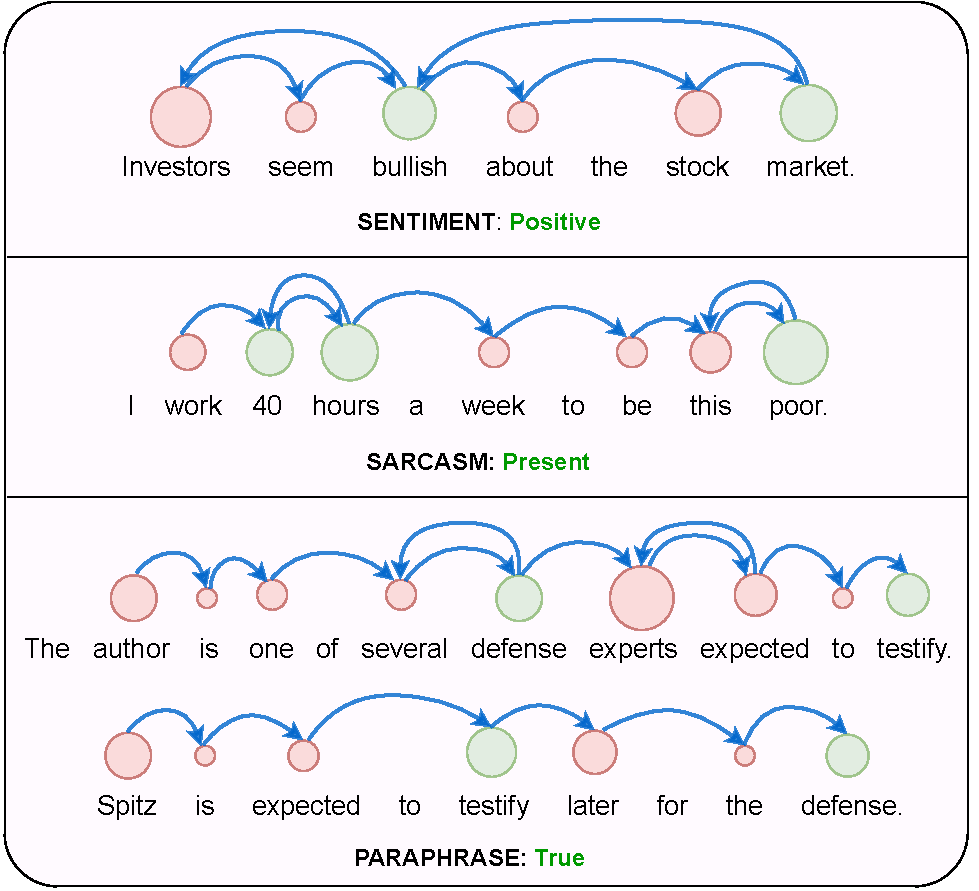
\includegraphics[width=1\columnwidth]{images/scanpath_sample_7.pdf}
    \caption{\small Generated scanpaths over text samples taken from various natural language processing (NLP) tasks. The green circles denote the important words characteristic of that task. The circles' size denotes the fixation duration, and the arrows depict the saccadic movements. As can be seen, linguistically important words often have a higher fixation duration and revisit. Regressions (word revisits) also appear in the examples. }
    \label{fig:scanpaths_for_NLP}
\end{figure}


\subsection{Introduction}

Integrating human signals with deep learning models has been beginning to catch up in the last few years. Digital traces of human cognitive processing can provide valuable signals for Natural Language Processing \cite{klerke2016improving,plank-2016-keystroke}. Various approaches for integrating human signals have been explored. For example, human feedback for better decisioning \citep{christiano2017deep}, NLP tasks \citep{stiennon2020learning,wu2021recursively}, and most recently language modeling using reinforcement learning with human feedback (RLHF) based reward \citep{bai2022training,ouyang2022training}. RLHF involves explicit human feedback and is expensive and hard to scale. On the other hand, previous studies have also tried to use implicit human feedback in the form of eyetracking signals.
%, human eye gaze for computer vision tasks like image captioning and visual question answering \citep{he2019human,boyd2022human}, and NLP tasks like sentiment analysis and NER \citep{NoraNEREyeTracking}.
It has proven to be a useful signal for inferring human cognitive processing \cite{sood2020improving, hollenstein-zhang-2019-entity, ijcaiSurveyGapIdentified}. NLP researchers have focused on assessing the value of gaze information extracted from large, mostly dis-jointly labeled gaze datasets in recurrent neural network models \cite{ren-xiong-2021-cogalign,strzyz-etal-2019-towards,barrett-etal-2018-sequence}. The proposed approaches under this paradigm include gaze as an auxiliary task in multi-task learning \cite{klerke-etal-2016-improving,hollenstein2019advancing}, as additional signals \cite{mishra-etal-2016-harnessing}, as word embeddings \cite{barrett-etal-2018-unsupervised}, as type dictionaries \cite{barrett-etal-2016-weakly,hollenstein-zhang-2019-entity}, and
as attention \cite{barrett-etal-2018-sequence}. 

Previous studies demonstrate that human scanpaths (temporal sequences of eye fixations, see Fig.~\ref{fig:scanpaths_for_NLP}) gleaned from eye tracking data improve the performance of NLP models. However, the real-world application of these methods remains limited primarily due to the cost of precise eye-tracking equipment, users' privacy concerns, and manual labor associated with such a setup. Therefore, generating scanpaths from existing eyetracking corpora would add great value to NLP research. To the best of our knowledge, this is the first work to propose a model that generates scanpaths for a given read text with good accuracy. We call the model, ScanTextGAN.

\iffalse
    \begin{figure}[!t]
        %\vspace{-35mm}
        \centering
        \includegraphics[width=.9\columnwidth]{images/scanpath_sample_5.pdf}
        %\vspace{-8mm}
        \caption{\small A sample human scanpath, i.e., a temporal sequence of eye fixations and saccades over words in a sentence. The size of the circles denotes the fixation durations, and the arrows depict the saccadic movements. Regressions (word revisits) can also be recognized.}
        \label{fig:scanpath_sample}
        %\vspace{-5mm}
    \end{figure}
\fi


\begin{figure}[!t]
    % \vspace{-3mm}
    \centering
    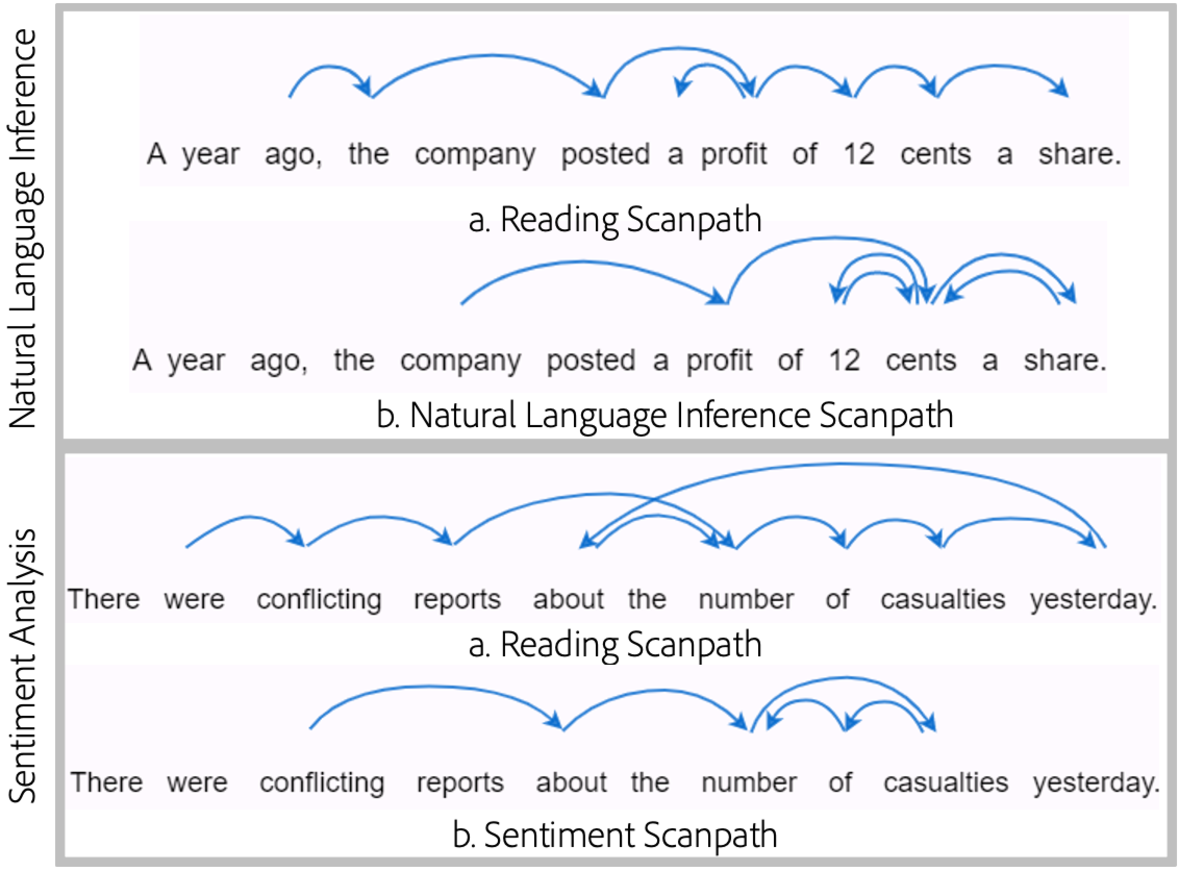
\includegraphics[width=0.7\columnwidth]{images/intent-scantextgan-scanpaths-3.pdf}
    %\vspace*{-2mm}
    \caption{\small (Intent-aware) Scanpath samples generated by conditioning scanpath generation on different downstream natural language tasks. Note that the conditioned scanpaths are heavily biased to words important for that downstream task.}
    \label{fig:intent-scanpaths-example} 
%\vspace{-3mm}
\end{figure}


We demonstrate the scanpath generation capability of ScanTextGAN over three eye-tracking datasets using multiple evaluation metrics. Further, we evaluate the utility of \textit{generated} scanpaths for improvements in the performance of multiple NLP tasks (see Figs.~\ref{fig:scanpaths_for_NLP},\ref{fig:intent-scanpaths-example}) including the ones in the GLUE benchmark \cite{wang-etal-2018-glue}. The generated scanpaths achieve similar performance gains as the models trained with real scanpaths for classic NLP tasks like sentiment classification, paraphrase detection, entailment, and sarcasm detection. 

Our contributions are threefold:

\noindent \textbf{1.} We propose ScanTextGAN, the first scanpath generator over text. \\
\textbf{2.} We compare ScanTextGAN with multiple baselines and conduct ablation experiments with varying models and configurations. The model performs well on the test sets and cross-domain generalization on two additional eyetracking datasets belonging to different text domains.\\
\textbf{3.} We tested the usefulness of generated scanpaths in downstream NLP tasks such as sentiment analysis, paraphrase detection, and sarcasm detection on six different datasets. The results show that the downstream NLP tasks benefited significantly from cognitive signals inherent in generated scanpaths. Further, we show how scanpaths change when finetuning with downstream natural language tasks (Figs.\ref{fig:intent-scanpaths-example},\ref{fig:intent-saliency-example}) and that they lead to further improvements in downstream task performance (\S\ref{sec:intent-scanpaths}) showing how they can act as additional controls beyond the task architecture.

% On six different datasets, we utilize the generated scanpaths to model downstream NLP tasks such as sentiment analysis, paraphrase detection, and sarcasm detection and show improved performance due to the cognitive signals contained in generated scanpaths. The results demonstrate that our model yields well-corroborated predictions with the human gaze on out-of-domain data.

%The rest of the paper is organized as follows. Section \ref{sec:RelatedWork} discusses the related work and identified research gap. Section \ref{sec:ProposedModel} illustrates the proposed model and datasets used for training, the training process, and loss functions, followed by Section \ref{sec:Performance Evaluation}, which summarizes the evaluation and discusses the results. Finally, Section \ref{sec:ConclusionFutureWork} concludes the paper considering possible future work.  




%%%%%%%%%%%%%%%%%%%%%%%%%%%%%%%%
\subsection{Related Work}
\label{sec:RelatedWork}

When reading a text, humans do not focus on every word and often do not read sequentially \cite{Just1980}. A series of studies in psycho-linguistics have shown that the number of fixations and the fixation duration on a word depend on several linguistic factors. The linguistic factors can also be determined given the cognitive features \cite{clifton2007eye, demberg2008data}.
Though advances in ML architecture have helped bring machine comprehension closer to human performance, humans are still superior for most NLP tasks \cite{blohm-etal-2018-comparing,xia-etal-2019-automatic}. 

It has been shown in the literature that integrating explicit \citep{bai2022training,ouyang2022training} and implicit (cognitive processing) human feedback signals in traditional ML models is expected to improve their performance \cite{Just1980}. However, the cost of explicit feedback (e.g., using MTurk) and implicit feedback (e.g., eye tracking) at scale is excessively high. Similarly, privacy-invasive eye-tracking processes limit the scope of this idea. One way to address this problem is to use generated eye movements to unfold the full potential of eye-tracking research. Hence, the idea is to architect ScanTextGAN, a scanpath generator for text reading, and test its usefulness in downstream NLP tasks. 

% Integrating human cognitive processing signals in traditional ML models is expected to improve performance \cite{Just1980}. However, the major hindrances is the unavailability and unacceptability of expensive and privacy-invasive eye-tracking process. One way to address this problem is to use generated eye movements to unfold the full potential of eye-tracking research. This motivated us to build the first scanpath generator for text, ScanTextGAN, and show its performance over both eye-tracking datasets and in downstream NLP tasks. Our work builds upon previous works on 1)~human attention modeling and 2)~gaze integration in neural network architectures.
More precisely, this work builds upon previous works on 1)~human attention modeling and 2)~gaze integration in neural network architectures, which are described as follows:

\textbf{Human Attention Modeling:} Predicting what people visually attend to in images (saliency prediction) is a long-standing challenge
in neuroscience and computer vision, the fields have seen many data-based models \cite{wang2021salient}. In contrast to images, most attention models for eye movement behaviors during reading are cognitive process models, \textit{i.e.}, models that do not involve machine learning but implement cognitive theories \cite{engbert2005swift,xia-etal-2019-automatic}. Key challenges for such models are a limited number of parameters and hand-crafted rules. Thus, it is difficult to adapt them to different tasks and domains and use them as part of end-to-end trained ML architectures \cite{kotseruba202040}. In contrast, learning-based attention models for text remain under-explored. Within that, all eye tracking models are saliency prediction models with non-existent work in predicting scanpaths. On the other hand, visual scanpaths generation for image-based eye tracking data has been recently explored for both traditional \cite{PathGANScanPathGen} and 360$^{\circ}$ images \cite{ScanGAN360}.

Matthies \textit{et al.} \cite{matthies-sogaard-2013-blinkers} presented the first fixation prediction work for text. They built a person-independent model using a linear Conditional Random Fields (CRF) model. %A separate line of work has instead tried incorporating assumptions about the human reading process into the model design. For \textit{e.g.}, 
Hahn and Keller \cite{hahn-keller-2016-modeling} designed the Neural Attention Trade-off (NEAT) language model, which was trained with hard attention and assigned a cost to each fixation. Other approaches include sentence representation learning using surprisal and part of speech tags as proxies to human attention \cite{10.5555/3171837.3171864}.%, attention as a way to improve time complexity for NLP tasks \cite{seo2018neural}, and learning saliency scores by training for sentence comparison \cite{samardzhiev-etal-2018-learning}.

Our work differs from previous studies as we combine cognitive theory and data-driven approaches to predict scanpaths and further show its application in downstream NLP tasks \cite{hollenstein-etal-2021-multilingual,hollenstein-etal-2021-cmcl}.

\begin{figure*}[!t]
%\vspace*{-12mm}
    \centering
    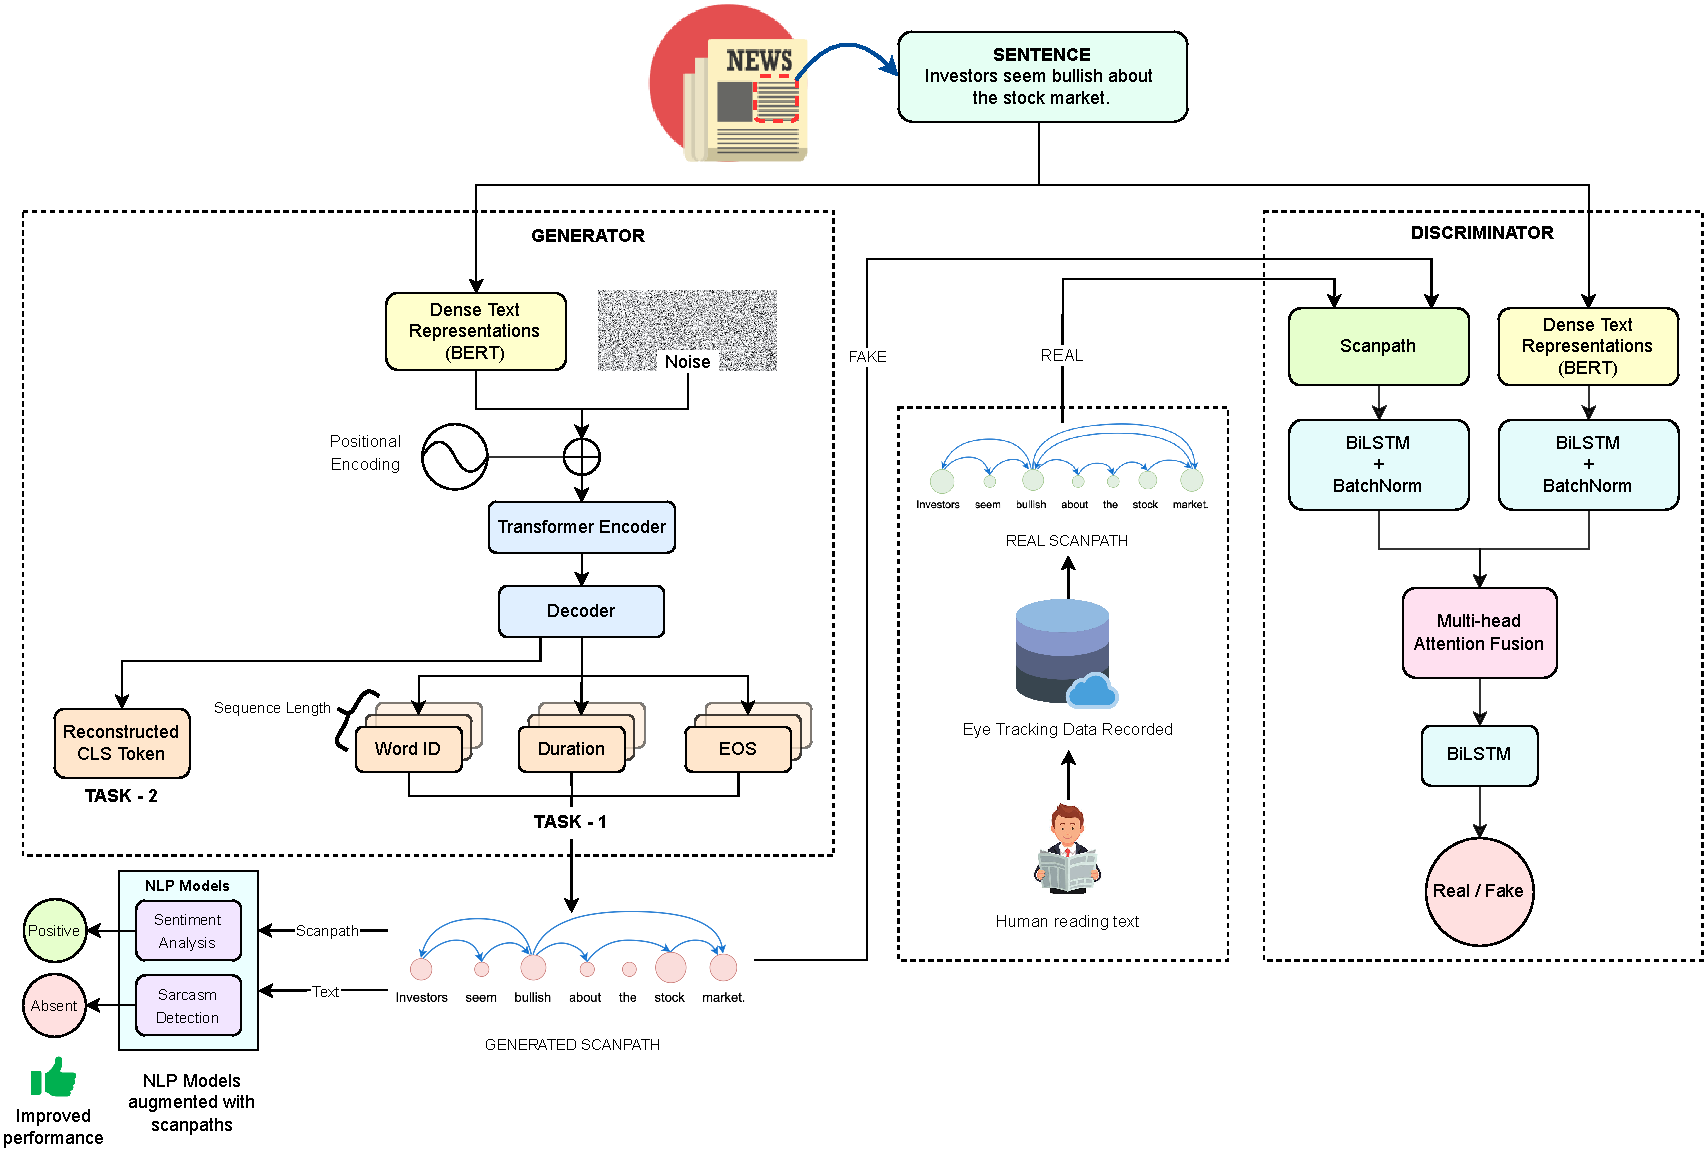
\includegraphics[width=\textwidth]{images/scanpath_model_6.pdf}
    %\vspace*{-2mm}
    \caption{The architecture of the proposed \textbf{ScanTextGAN} model. The model consists of a conditional generator and a discriminator playing a zero-sum game. The generator is trained by two cognitively inspired losses: text content reconstruction and scanpath content reconstruction.}
    \label{fig:model} 
%\vspace*{-3mm}
\end{figure*}

\textbf{Integrating Gaze in Network Architecture:} Integration of human gaze data into neural network architectures has been explored for a range of computer vision tasks such as image captioning, visual question answering, and tagging \cite{karessli2017gaze,yu2017supervising,he2019human,boyd2022human}. %In language processing, tracking a reader's eye movements provides information about the cognitive processes of text comprehension \cite{RaynerReadingComp, Just1980}. 
Hence, recent research has utilized features gleaned from readers' eye movement to improve the performance of complex NLP tasks such as sentiment analysis \cite{long-etal-2017-cognition, mishra-etal-2016-leveraging}, sarcasm detection \cite{mishra-etal-2016-harnessing}, part-of-speech tagging \cite{barrett-etal-2016-cross}, NER \cite{hollenstein-zhang-2019-entity}, and text difficulty \cite{ScanPathApp1}.

While in recent years, eye tracking data has been used to improve and evaluate NLP models, the scope of related studies remains limited due to the %one of the main limitations of these methods of cognitively-inspired NLP is the %limited availability of large datasets and the 
requirement of real-time gaze data at inference time. Mathias \textit{et al.} \cite{ijcaiSurveyGapIdentified} reported that there exists no automated way of generating scanpaths yet in the literature. With high-quality artificially generated scanpaths, the potential of leveraging eyetracking data for NLP can be unfolded. Additionally, generating scanpaths that mimic human reading behavior will help advance our understanding of the cognitive processes behind language understanding. Hence, we propose ScanTextGAN; researchers can use that to generate scanpaths over any text without worrying about collecting them from real users. 

%We show the utility of the generated scanpaths by achieving performance gains in downstream NLP tasks over six corpora.

\subsection{Proposed Model}
\label{sec:ProposedModel}
In this section, we define the scanpath generation task, describe the ScanTextGAN model architecture, and provide details on loss functions and model training.

\textbf{Task Definition:} The task of scanpath generation is to generate a sequence $\mathcal{S}(\mathcal{T})$ representing a scanpath over the text $\mathcal{T} = \{w_1,w_2,...,w_n\}$ composed of a sequence of words, can be defined as follows:
\begin{equation}
    \mathcal{S(T)} = \{..,(w_a^i,t^i),....,(w_b^j,t^j),....,(w_c^k,t^k)\}
\end{equation}
where $t^i$ represents the fixation duration over the word $w_a$ occurring at the position $i$.  Note that it is not necessary to have $a<b$ (words being read in linear order) or that $k=n$ (the number of fixations being equal to the number of words). Due to regressions, \textit{i.e.}, backward saccades to previous words, words are also revisited. Hence, the same word could appear multiple times in the sequence.

\subsubsection{ScanTextGAN Model Architecture}
Fig.~\ref{fig:model} illustrates the proposed conditional GAN architecture of the model. The ScanTextGAN model is composed of two competing agents. First, a conditional generator that generates scanpaths given text prompts. The second is a discriminator network, which distinguishes real human scanpaths from the generated ones. The ScanTextGAN model is trained by combining text content loss, scanpath content loss, and adversarial loss (Eq.~\ref{eq:Net Generator Loss}). The scanpath content loss measures the difference between the predicted scanpath and the corresponding ground truth scanpath. The text content loss reconstructs the input text, and the adversarial loss depends on the real/synthetic prediction of the discriminator over the generated scanpath. We describe the losses along with the generator and discriminator architectures next.

\looseness=-1 \textbf{Generator:} The ScanTextGAN generator constitutes a transformer-based encoder-decoder framework. The encoder is conditioned on BERT-based text embeddings \cite{devlin2018bert}, which are concatenated with noise to make the generator's output non-deterministic. The output of the transformer encoder is supplied to the decoder, which consists of task-specific feed-forward networks. One branch generates the scanpath (\textit{Task 1}), while the other reconstructs the $768$ dimensional CLS token embedding of the sentence (\textit{Task 2}). The scanpath is output as a temporal sequence of word ID (fixation points) $w_a^i$, fixation duration $t^i$, and end-of-sequence probability $EOS^i$. At inference time, the length $L(G)$ of generated scanpath $G$ is determined as follows:


\begin{equation}
L(G) = \begin{cases}
          \min_{1 \leq k \leq M} (k) \quad &\text{if} \, EOS^k > \tau \\
          M \quad &\text{otherwise} \, \\
     \end{cases}
\end{equation}
where $M$ is the maximum scanpath length as described in section \S\ref{sec:dataset} and $\tau \in (0,1)$ is a probability threshold. We use $\tau = 0.5$. The loss functions of the two branches are described below. 


\looseness=-1 \textbf{Scanpath Content Loss} tries to minimize the deviation of generated scanpaths $\mathcal{G}(\mathcal{T}, \mathcal{N})$ from the ground-truth scanpaths $\mathcal{R}(\mathcal{T}, h))$ over text $\mathcal{T}$ where ground-truth scanpaths are recorded from the human $h$ and $\mathcal{N}$ stands for Gaussian noise $\mathcal{N}(0, 1)$. The loss function $\mathbb{L}_s$ is given as:
\begin{equation}
    \label{eq:Scanpath Content Loss}
    \begin{aligned}
    \mathbb{L}_s(\mathcal{G}(\mathcal{T,}\mathcal{N}), \mathcal{R}(\mathcal{T},h)) = \frac{1}{k} \Sigma_{i=0}^{k}(&\alpha(id_g^i-id_r^i)^2 + \\ \beta(t_g^i-t_r^i)^2 + &\gamma (E_g^i-E_r^i)^2)
    % \\+ &\gamma P_g(E^i)*log(P_r(E^i)))
    \end{aligned}
\end{equation}
which is a weighted sum of three terms. The first term measures the error between real and predicted \textit{fixation points} given by the mean squared difference between generated and real word-ids $(id_g^i-id_r^i)$. It penalizes permutations of word ids and trains the model to approximate the real sequence of fixation points closely.

The second term measures the difference in \textit{fixation durations} given by the mean squared difference between generated and real duration $(t_g^i-t_r^i)$. Fixation durations simulate human attention over words in the input text. Thus, a word with a larger fixation duration is typically synonymous with greater importance than other words in the input text. This error term supplements the generator's ability to learn human attention patterns over the input text.

Finally, the third term measures the mean squared error between the prediction of end-of-sequence probability by real and generated distributions $(E_g^i-E_r^i)$. These are weighted by the hyperparameters $\alpha,\beta$, and $\gamma$. Preliminary experiments showed that optimizing the mean squared error leads to better performance over the cross-entropy loss for optimizing the EOS probability output.

\looseness=-1 \textbf{Text Content Loss:} Scanpaths depend heavily on the linguistic properties of the input text. Therefore, to guide the generator towards near the probable real data manifolds, we adopt reconstruction of the CLS token embedding of the input text (\textit{Task 2}) by the generator as an auxiliary task since the CLS token embedding encodes a global representation of the input text. 
This text content reconstruction loss $\mathbb{L}_r$ is given as: 
\begin{equation}
    \label{eq:Text Content Loss}
    \begin{aligned}
     \mathbb{L}_r(\mathcal{G}(\mathcal{T,}\mathcal{N}), \mathcal{R}(\mathcal{T},h)) = (&BERT(w_i^g,w_j^g,...,w_k^g\\-&BERT(w_a^r,w_b^r,...w_n^r))^2
    \end{aligned}
\end{equation}
where $BERT(w_a^r,w_b^r,...w_n^r)$ and $BERT(w_i^g,w_j^g,...w_k^g)$ stand for the \textit{CLS} vector representations of real and generated text respectively.

\textbf{Discriminator:} The goal of the discriminator is to distinguish between the real and synthetic scanpaths supplied to it. Similar to the generator, it requires text representations to distinguish between real and generated scanpaths. Specifically, the discriminator comprises two blocks of BiLSTMs that perform sequential modeling over the scanpaths and BERT embeddings. The outputs of the two branches are combined and passed to an attention fusion module with four heads, followed by another network of BiLSTMs. The hidden states of the last BiLSTM layer from both forward and backward directions are concatenated and supplied to a feed-forward network. A Sigmoid function activates the output of the feed-forward network. In this manner, the discriminator classifies the input scanpaths as either \textit{real} or \textit{fake}.

\textbf{Adversarial Loss:} The generator and discriminator networks are trained in a two-player zero-sum game fashion. The loss is given by:
\begin{equation}
    \label{eq:Adversarial Loss}
    \begin{aligned}
    \mathbb{L}_a = \min_{G}\max_{D}\mathbb{E}_{x\sim p_{\text{data}}(x)}[\log{D(x|\mathcal{T},h)}] + \\  \mathbb{E}_{z\sim p_{\text{z}}(z)}[1 - \log{D(G(z|\mathcal{T,N}))}]
    \end{aligned}
\end{equation}
Therefore, the net generator loss becomes:
\begin{equation}
    \label{eq:Net Generator Loss}
    \begin{aligned}
    \mathbb{L}_g = \mathbb{L}_s + \mathbb{L}_r + \mathbb{E}_{z\sim p_{\text{z}}(z)}[1 - \log{D(G(z|\mathcal{T,N}))}]
    \end{aligned}
\end{equation}

\subsubsection{Dataset} 
\label{sec:dataset}
\looseness=-1 For training the ScanTextGAN model, we use the CELER dataset \cite{berzak2022celer}. It contains eyetracking data of 365 participants for nearly 28.5 thousand newswire sentences, sourced from the Wall Street Journal Penn Treebank \cite{marcinkiewicz1994building}. Each participant in CELER reads 156 newswire sentences. Half of the sentences are shared across participants, and the rest is unique to each participant. The maximum sentence length was set to 100 characters. Participant eyetracking data were recorded using Eyelink 1000 tracker in a desktop mount configuration with a sampling rate of 1000 Hz. The ScanTextGAN model is trained to approximate the average eye movements of all the participants who read given sentences. The CELER dataset was envisioned to enable research on language processing and acquisition and to facilitate interactions between psycholinguistics and natural language processing. Furthering the goal, we use it to train our conditional GAN model through which we show human scanpath approximation capabilities (\S\ref{sec:Evaluation of Scanpath Generation}). Also, we use it to show improvements in the performance of NLP tasks (\S\ref{sec:Application to NLP Tasks}). 

\looseness=-1
The data consist of tuples of participant ID, sentence ID, and word ID corresponding to fixation point and fixation duration. We compute the 99th percentile of fixation durations and treat it as the largest value. Fixations of durations longer than this are treated as outliers and hence dropped from the dataset. To apply the scanpath reconstruction loss (Eq.~\ref{eq:Scanpath Content Loss}), we scale all fixation durations by the maximum value and then normalize them to [0,1]. Similarly, word IDs in each sentence are normalized to [0, 1] after scaling them by the length of that sentence. For the last fixation point in every scanpath, the binary EOS token is set to 1. The maximum scanpath length is set to 80 fixation points (99th percentile of the lengths). Thus shorter scanpaths are padded while longer scanpaths are trimmed. We use BERT to encode the sentences and obtain their $768$-dimensional embeddings, keeping the max length parameter as 80, thus resulting in an $80\times768$ dimensional tensor.

\subsubsection{Parameter Settings}
\looseness=-1
Sinusoidal positional encoding is applied over the input embeddings fed to the generator. We use a 3-layer transformer encoder with four head attention and a hidden dimension size of 776 in the generator. In the discriminator, we use bidirectional LSTMs over sentence embeddings and generated scanpaths with a hidden size of 64 and a dropout ratio of 0.3, followed by batch normalization for faster convergence. An attention module with four attention heads is applied after concatenating the outputs.
We employ the Adam and RMSProp optimizer to minimize generator and discriminator losses. The batch size is set to 128, the initial learning rate of the generator to 0.0001, and that of the discriminator to 0.00001. The model is trained for 300 epochs. Our implementation uses PyTorch, a popular deep-learning framework in Python. All experiments are run on an Intel Xeon CPU with Nvidia A100-SXM GPUs.



\subsection{Performance Evaluation}
\label{sec:Performance Evaluation}
We quantify the performance of ScanTextGAN in two regimes\footnote{All results are calculated with five random seeds and reported as the mean of those five runs}; first, scanpath generation with three datasets, and second, NLP tasks with six datasets. Similar to prior computer vision studies \cite{sun2019visual,de2022scanpathnet,kummerer2021state,jiang2016learning}, we evaluate the ScanTextGAN model over the scanpath generation task. For this, we use the test split of the CELER dataset, Mishra \textit{et al.} (2016) \cite{mishra2016predicting}, and Mishra \textit{et al.} (2017) \cite{Mishra_Kanojia_Nagar_Dey_Bhattacharyya_2017}. In addition, unlike the computer vision studies, we also evaluate the ScanTextGAN model for improvement in NLP tasks. The hypothesis is that the human eyes (and consequently the brain) process many language comprehension tasks unconsciously and without visible effort. The next logical step is to capture (or, in our case, generate) this mental representation of language understanding and use it to improve our machine-learning systems. For evaluation, we use four tasks from the GLUE benchmark and two from the tasks proposed by \cite{mishra2016predicting}. While the ScanTextGAN model is trained over news text from the CELER dataset, with the help of the other datasets, we expand our testing to other domains, including reviews, quotes, tweets, and Wikipedia text. 


\subsubsection{Evaluation Datasets}
\label{sec:eval_datasets}
\textbf{Mishra \textit{et al.} (2017) \cite{Mishra_Kanojia_Nagar_Dey_Bhattacharyya_2017}} comprises eye movements and reading difficulty data recorded for 32 paragraphs on 16 different topics, \textit{viz.} history, science, literature, \textit{etc}. For each topic, comparable paragraphs were extracted from Wikipedia\footnote{\url{https://en.wikipedia.org/}} and simple Wikipedia\footnote{\url{https://simple.wikipedia.org/}}. The participant's eye movements are tracked using an SR-Research Eyelink-1000 Plus eye tracker. Using the ground truth scanpaths over the text corpora, we evaluate the quality of generated scanpaths.


\textbf{Mishra \textit{et al.} (2016) \cite{mishra2016predicting}} contains eye fixation sequences of seven participants for 994 text snippets annotated for sentiment and sarcasm. These were taken from Amazon Movie Corpus %\cite{pang-lee-2004-sentimental}
, Twitter, and sarcastic quote websites. %They used an SR-Research Eyelink-1000 eye-tracker to collect the eye movements of the participants. 
The task assigned to the participants was to read one sentence at a time and annotate it with binary sentiment polarity labels (\textit{i.e.}, positive/negative). %Using feature engineering approaches, 
%They used the scanpath data to show improvements in sarcasm detection. 
The same datasets were used in several studies \cite{joshi-etal-2015-harnessing,mishra-etal-2016-harnessing,mishra-etal-2016-leveraging} to show improvements in sarcasm and sentiment analysis.
We use the datasets to evaluate both the generation quality and potential improvements in NLP tasks.% using generated scanpaths, thereby making it more aligned with real-world settings and solving the problem of the unavailability of human scanpath data at inference time.


\begin{table*}[!t]\centering
% \scriptsize
\resizebox{\textwidth}{!}{\begin{tabular}{lcccccc}\toprule
\multirow{2}{*}{\textbf{Generator Model}} &\multicolumn{4}{c}{\textbf{MultiMatch $\uparrow$}} &\multirow{2}{*}{\textbf{Levenshtein Distance $\downarrow$}} \\\cmidrule{2-5}
&\textbf{Vector$\uparrow$} &\textbf{Length$\uparrow$} &\textbf{Position$\uparrow$} &\textbf{Duration$\uparrow$} & \\\midrule
Inter-subject score\footnotemark & 0.973   & 0.958 &    0.830   & 0.698 & 0.691\\\midrule
%Transformer Encoder-Decoder &0.974 &0.958 &\textbf{0.819} &0.543 & \\
%Transformer Encoder &0.974 &0.957 &0.773 &0.703 & \\
LSTM Encoder-Decoder trained with scanpath content loss & 0.975 & 0.956 &  0.765 & 0.344 & 0.865\\
ScanTextGAN -- Text Reconstruction -- GAN Loss& 0.968 & 0.947 & 0.728 & 0.703 & 0.779\\
\textbf{ScanTextGAN} &\textbf{0.983} &\textbf{0.972} & \textbf{0.787} & 0.733 & \textbf{0.769}\\
ScanTextGAN -- Text Reconstruction &0.974 &0.957 &0.773 &0.703 & 0.798\\
ScanTextGAN -- GAN Loss &0.973 &0.955 &0.750 &\textbf{0.761} &0.786\\
% *ScanTextGAN + Dwell Time reconstruction & 0.960 & 0.932 & \textbf{0.805} & 0.711 \\
% *Dwell Time reconstruction w/o Adv. training & 0.966 &0.939	&0.786 &0.775 \\
ScanTextGAN + addition of noise &0.971 &0.952 &0.756 &0.736 &0.791\\
ScanTextGAN -- Text (CLS) Reconstruction + sentence reconstruction &0.978 &0.963 &0.724 &0.721 &0.805 \\
% \midrule
% Inter-Subject Scanpath Topline & XXX & & & & 
% \\ 
\bottomrule
\end{tabular}}
\caption{In-domain Evaluation of Scanpath Generation on the CELER dataset \cite{berzak2022celer}.}\label{tab:celer}
\end{table*}


\footnotetext{In the CELER dataset, there are only 78 shared sentences amongst all the participants. Therefore, inter-subject scanpath evaluation is done only for these sentences. In contrast, the ScanTextGAN results are reported for the entire test set (including these 78 sentences).}


Furthermore, we explore the potential of including cognitive signals contained in scanpaths in NLP models for a range of GLUE tasks which include Sentiment Analysis using Stanford Sentiment Treebank (SST), Paraphrase Detection using Microsoft Research Paraphrase Corpus (MRPC) and Quora Question Pairs (QQP), Natural Language Inference using Recognizing Textual Entailment (RTE) dataset.
%- \textbf{SST}: The Stanford Sentiment Treebank includes fine-grained sentiment labels for 215154 phrases in the parse trees of 11855 sentences. The corpus consists of sentences from movie reviews and human sentiment annotations. The task is to predict the sentiment of a given sentence. We use the two-way (positive/negative) class split and only sentence-level labels.\\
%- \textbf{MRPC}: The Microsoft Research Paraphrase Corpus comprises a set of 5,801 sentence pairs collected from newswire articles. Each pair is annotated with a label indicating whether the sentences are paraphrased or not.\\
% Each pair is labeled whether human annotators paraphrase it. The dataset is divided into \textit{train} (4,076 sentence pairs, of which 2,753 are paraphrases) and \textit{test} (1725 pairs, of which 1,147 are paraphrases).\\
%- \textbf{QQP}: The Quora Question Pairs (QQP) dataset consists of over 400,000 question pairs. Each is annotated with a binary value indicating whether the two questions are paraphrases of each other. \\
%- \textbf{RTE}: The Recognizing Textual Entailment (RTE) dataset involves a generic Natural Language Inference task that recognizes, given a pair of texts, whether the meaning of one text can be inferred from the other. 

Next, we cover the results of scanpath generation and its application in NLP tasks.



\begin{figure}[]
    \centering
    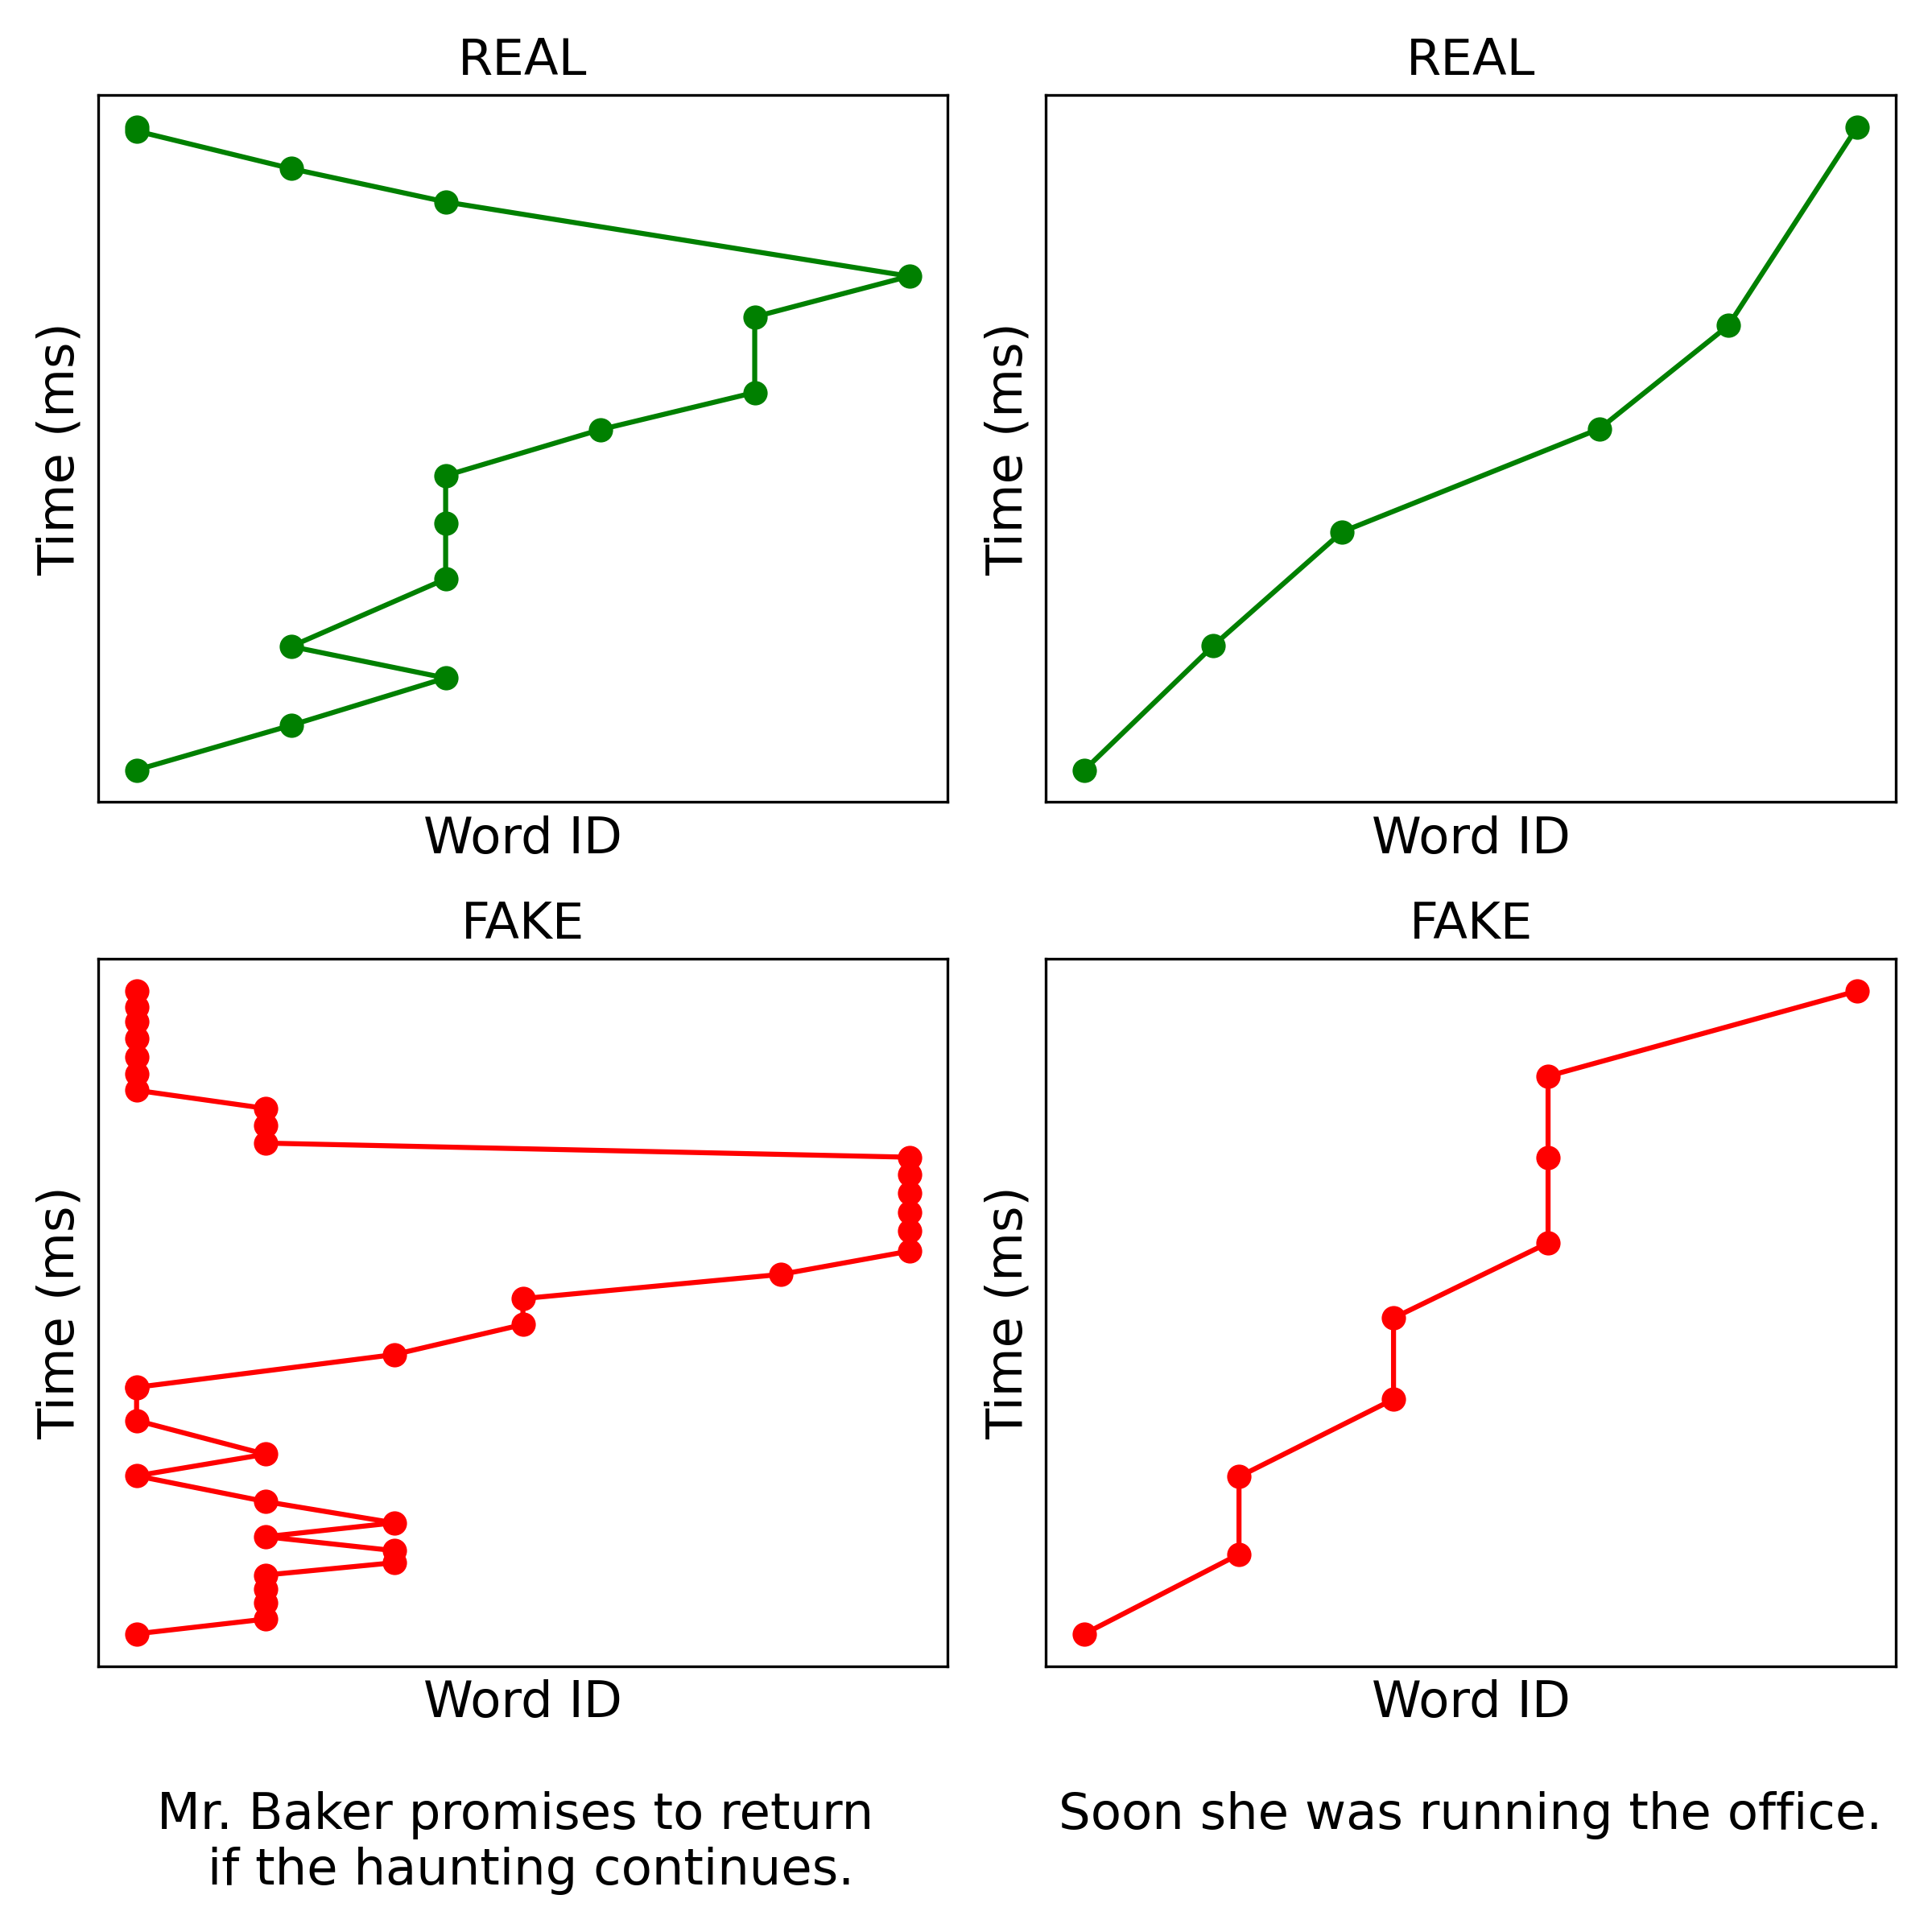
\includegraphics[width=0.7\columnwidth]{images/scanpath_plot_combined_sent_5.png}
    \caption{Comparison of \textit{real} and \textit{synthesized} scanpaths corresponding to a few text samples. The proposed ScanTextGAN model generates the latter.}
    \label{fig:scanpath_comparison}
\end{figure}


\subsubsection{Evaluation of Scanpath Generation}
\label{sec:Evaluation of Scanpath Generation}
We evaluate the scanpath generation model on two most commonly used metrics in image scanpath generation studies \cite{sun2019visual,chen2018scanpath,de2022scanpathnet,kummerer2022deepgaze}: \textbf{MultiMatch} \cite{jarodzka2010vector} and \textbf{Levenshtein Distance} \cite{levenshtein1965leveinshtein}. Multimatch is a geometrical measure that compares scanpaths across a comprehensive set of dimensions composed of shape, lengths, position, and fixation duration. Levenshtein Distance between a pair of sequences measures the least number of edits (inserts, deletes, substitution) to transform one into the other.

\paragraph{Scanpath Evaluation Metrics}
\label{sec:appendix_scanpath_metrics}

\textbf{MultiMatch} is a geometrical measure that models scanpaths as vectors in 2-D space, wherein the vectors represent saccadic eye movements. Starting and ending coordinates of these saccades constitute the fixation positions. It compares scanpaths across multiple dimensions, \textit{viz.} shape, length, position, direction, and fixation duration. Shape measures the vector difference between aligned saccade pairs, which is then normalized by twice the diagonal screen size. Length measures the normalized difference between the endpoints of real and generated saccade vectors. Direction is the angular distance between the two vectors. The position is the Euclidean difference in position between aligned vectors, and duration measures the difference in fixation durations normalized against the maximum duration. Since our work deals with scanpaths over text, we use 1-D space to represent the saccade vectors where word IDs denote the fixation positions. Thus, it is easy to see that computing scanpath direction similarity is redundant here (it is subsumed within position); hence we drop it from our analysis. 


\textbf{Levenshtein Distance} between a pair of sequences measures the least number of character edits, i.e., insertion, deletion, and substitution needed to transform one sequence into the other.
Specifically, we use it to gauge the degree of dissimilarity between a pair of real $R$ and generated $G$ scanpaths. To account for the fixation durations of each word, $R$ and $G$ are temporally binned using a $50$ ms bin size, similar to the computation of ScanMatch metric \cite{cristino2010scanmatch}. The resulting sequences of word IDs, $R_W$ and $G_W$ are transformed into character strings, $R_S = \{r_1, r_2, ..., r_n\}$ and $G_S = \{g_1, g_2, ...,g_m\}$, where $R_S$ and $G_S$ are strings over the ASCII alphabet and $n = |R_S|$ and $m = |G_S|$.
Thus, a lower NLD score is indicative of greater scanpath similarity. 


Further, as a top-line comparison, we use \textbf{inter-subject scanpath similarity} \cite{sun2019visual}. It measures the degree of variation among real human scanpaths corresponding to each text input. To compute this, we first calculate each subject's performance by treating the scanpaths of other subjects as the ground truth. Then, the average value of all subjects is used as inter-subject performance.


\textbf{Baselines:} Since ScanTextGAN is the first text-based scanpath generation model, we conduct an ablation study to compare ScanTextGAN with its other variants. Specifically, we compare ScanTextGAN with the following six configurations: (1)~An LSTM-based network trained with scanpath content loss. Sentence embeddings obtained through BERT are concatenated with noise in this model. The resultant is fed to an attention module with four heads, then passed to a network of LSTMs and Batch Normalization layers applied in tandem. (2)~ScanTextGAN model trained with only the scanpath content loss. (3)~ScanTextGAN model without the text reconstruction loss (Task-2). (4)~ScanTextGAN model with BERT-based sentence embeddings reconstruction instead of CLS token reconstruction. (5)~ScanTextGAN model with the addition of noise instead of concatenation. (6)~ScanTextGAN model trained without GAN loss.



\begin{table*}[!t]\centering
% \scriptsize
\resizebox{\textwidth}{!}{\begin{tabular}{lcccccc}\toprule
\multirow{2}{*}{\textbf{Generator Model}} &\multicolumn{4}{c}{\textbf{MultiMatch $\uparrow$}} &\multirow{2}{*}{\textbf{Levenshtein Distance $\downarrow$}} \\\cmidrule{2-5}
&\textbf{Vector$\uparrow$} &\textbf{Length$\uparrow$} &\textbf{Position$\uparrow$} &\textbf{Duration$\uparrow$} & \\\midrule
Inter-subject score & 0.977   & 0.963 &    0.839   & 0.715 & 0.723\\\midrule
LSTM Encoder-Decoder trained with scanpath content loss& \textbf{0.984}    & \textbf{0.973} &   0.714 &   0.379 & 0.918\\
ScanTextGAN -- Text Reconstruction -- GAN Loss& 0.977   & 0.960 &    0.780   & 0.769 & 0.847\\
%Transformer Encoder-Decoder &0.977 &0.957 &0.821 &0.574 & \\
%Transformer Encoder &0.976 &0.961 &0.763 &0.757 & \\
\textbf{ScanTextGAN} &0.966 &0.945 &\textbf{0.791} &\textbf{0.771} & \textbf{0.836} \\
ScanTextGAN -- Text Reconstruction &0.976 &0.961 &0.763 &0.757 & 0.845\\
% *ScanTextGAN + Dwell Time reconstruction & 0.971 &0.952 & \textbf{0.797} &0.711 \\
% *Dwell Time reconstruction w/o Adv. training & 0.976 &0.959	&0.795 &0.765 \\
ScanTextGAN -- GAN Loss &0.976 &0.959 &0.774 &0.768 &0.839\\
ScanTextGAN + addition of noise &0.968 &0.947 &0.737 &0.743 & 0.838\\
ScanTextGAN -- Text (CLS) Reconstruction + sentence reconstruction &0.964 &0.934 &0.747 &0.733 & 0.869\\
\bottomrule
\end{tabular}}
\caption{Cross-domain Evaluation of Scanpath Generation on the Dataset by \cite{mishra2016predicting}.}\label{tab:iitb_2016}
%\vspace*{-3mm}
\end{table*}

\begin{table*}[!t]\centering
% \vspace*{-10mm}
% \scriptsize
\resizebox{\textwidth}{!}{\begin{tabular}{lcccccc}\toprule
\multirow{2}{*}{\textbf{Generator Model}} &\multicolumn{4}{c}{\textbf{MultiMatch $\uparrow$}} &\multirow{2}{*}{\textbf{Levenshtein Distance $\downarrow$}} \\\cmidrule{2-5}
&\textbf{Vector$\uparrow$} &\textbf{Length$\uparrow$} &\textbf{Position$\uparrow$} &\textbf{Duration$\uparrow$} & \\\midrule
Inter-subject score & 0.994   & 0.991 &    0.834   & 0.620 & 0.845\\\midrule
LSTM Encoder-Decoder trained with scanpath content loss& \textbf{0.992}  &  \textbf{0.987}   & 0.596 &    0.329 & 0.969\\
ScanTextGAN -- Text Reconstruction -- GAN Loss&0.990 &0.984 &0.729 &0.705 & 0.951\\
%Transformer Encoder &0.986 &0.981 &0.776 &0.706 & \\
\textbf{ScanTextGAN} &0.984 &0.977 &\textbf{0.759} &0.693 & \textbf{0.931}\\
ScanTextGAN -- Text Reconstruction &0.986 &0.981 &0.756 &\textbf{0.706} & 0.939\\
% *ScanTextGAN + Dwell Time reconstruction & 0.985 &0.977	&\textbf{0.773}	&0.605 \\
% *Dwell Time reconstruction w/o Adv. training &0.990	&0.985 &0.686	&0.701 \\
ScanTextGAN -- GAN Loss &0.990 &0.984 &0.739 &\textbf{0.706} &0.945\\
ScanTextGAN + addition of noise &0.984 &0.976 &0.759 &0.703 & 0.943\\
ScanTextGAN -- Text (CLS) Reconstruction + sentence reconstruction &0.983 &0.974 &0.667 &0.674 & 0.958\\
\bottomrule
\end{tabular}}
\caption{Cross-domain Evaluation of Scanpath Generation on the Dataset by \cite{Mishra_Kanojia_Nagar_Dey_Bhattacharyya_2017}.}\label{tab:iitb_2017}
%\vspace*{-3mm}
\end{table*}



\textbf{Results:} Table~\ref{tab:celer} presents the results of our scanpath prediction model on the CELER dataset. Further, we also compare ScanTextGAN with baselines on two other contemporary datasets of movie reviews, tweets, and sarcastic quotes \cite{mishra2016predicting},  Wikipedia and simple Wikipedia paragraphs  \cite{Mishra_Kanojia_Nagar_Dey_Bhattacharyya_2017}. Tables~\ref{tab:iitb_2016} and \ref{tab:iitb_2017} present the results of our model on those datasets. For obtaining results on these corpora, we use the model trained on the CELER dataset, thus helping us evaluate the cross-domain performance of the model. 

As can be seen in Table~\ref{tab:celer}, Table~\ref{tab:iitb_2016} and Table~\ref{tab:iitb_2017}, ScanTextGAN outperforms other models for scanpath prediction on most metrics. The performance of ScanTextGAN even surpasses inter-subject reference on Duration and comes very close to Vector, Length, and Position. 

We observe that adopting the reconstruction of the CLS token as an auxiliary task (Task - 2) boosts the model performance. Reconstructing the full sentence embeddings rather than the CLS tokens only as an auxiliary task does not always improve the results, despite adding a larger computational overhead. The results also reveal that concatenating noise with text embeddings is more rewarding than adding it.

Further, to compare the skipping behavior of ScanTextGAN with humans, we calculate the weighted F1 score of the words skipped and attended by both model types. We find the weighted F1 to be 64.6 between them. Fig.~\ref{fig:scanpath_comparison} presents a visual comparison between real scanpaths from the available eyetracking data and scanpaths generated by ScanTextGAN, corresponding to some randomly chosen text samples. We can observe that the generated scanpaths resemble the real ones to a great extent. Thus, the quantitative and qualitative results on in-domain and cross-domain settings lead us to believe that our proposed scanpath generation model can be deemed a good approximator of the human scanpaths. % and can be used for downstream NLP applications.


%%%%%%%%%%%%%%%%%%%%%%%%%%%%%%%%%%%%%%%%%%%%%%%%%%%%%%%%%%%%%%%%%%
%%%%%%%%%%%%%%%%%%%%%%%%%%%%%%%%%%%%%%%%%%%%%%%%%%%%%%%%%%%%%%%%%%
\subsubsection{Application to NLP Tasks}
\label{sec:Application to NLP Tasks}
% \begin{table}[t]\centering
% \caption{Sentiment analysis and sarcasm detection results on the dataset by \cite{mishra2016predicting}. Model configuration refers to the type of scanpath included in train and test data.}
% \label{tab:iitb_classifier_results}
% % \scriptsize
% \begin{tabular}{cc|ccc}\toprule
% \multicolumn{2}{c}{\textbf{Model Configuration}} &\multicolumn{2}{c}{\textbf{Weighted F1 score}} \\\cmidrule{1-4}
% \textbf{Train} & \textbf{Test} &\textbf{Sentiment} &\textbf{Sarcasm} \\\midrule
% None &None &0.7839 &0.9438 \\
% Real &Real &0.8334 &0.9501 \\
% Random &Generated &0.7773 &0.9313 \\
% Real &Generated &0.8319 &0.9378 \\
% Generated &Real &0.8402 &0.9452 \\
% Generated &Generated &0.8332 &0.9506 \\
% Real+Generated &Generated &\textbf{0.8404} &\textbf{0.9512} \\
% \bottomrule
% \end{tabular}
% \end{table}

% \usepackage{booktabs}

We use them to augment various NLP models and measure their performance to demonstrate the usefulness of cognitive signals hidden in the \textit{generated} scanpaths.

\textbf{Sentiment Classification and Sarcasm Detection:} For these tasks, we use a model consisting of a network of two branches of BiLSTMs and Batch Normalization layers that perform sequential modeling over text representations obtained through BERT and scanpaths fed as input to the model. The outputs of both branches are combined and passed to another layer of BiLSTMs, followed by a feed-forward network that predicts binary sentiment/sarcasm labels corresponding to the input after activating with the Sigmoid function. We follow a 10-fold cross-validation regime.

We compare the models with generated scanpaths, real scanpaths, and without scanpaths. Further, to investigate whether performance gains observed by adding scanpaths are due to scanpaths and not the increase in the number of parameters, we train a \textit{Random-Random} variant in which we send Random noise as scanpaths to the model with an increased number of parameters. We also simulate the real-world case where both real and generated scanpaths are available during train time, but only generated ones are available during test time, for example, during user deployment. 
%We also compare the results for all tasks with models fed with random noise as scanpaths. 
\begin{table}[!t]
\centering
% \vspace{-10mm}
\begin{tabular}{llcc} 
\toprule
\multicolumn{2}{c}{\textbf{Model Configuration}} & \multicolumn{2}{c}{\textbf{F1 score}}  \\ 
\midrule
\textbf{Train}   & \textbf{Test}                 & \textbf{Sentiment} & \textbf{Sarcasm}           \\ 
\midrule
w/o              & w/o                           & 0.7839             & 0.9438                     \\
Random           & Random                     & 0.7990             & 0.9397    \\
Random           & Generated                     & 0.7773             & 0.9313                     \\
Real             & Generated                     & 0.8319             & 0.9378                     \\
Real      & Real        & 0.8334        & 0.9501             \\
Generated        & Real                          & 0.8402             & 0.9452                     \\
Generated        & Generated                     & 0.8332             & 0.9506                     \\
Real + Generated & Generated                     & \textbf{0.8404}    & \textbf{0.9512}            \\ \midrule

Intent-Aware & Intent-Aware & \textbf{0.8477} & \textbf{0.9528} \\ \bottomrule
\end{tabular}
\caption{Sentiment analysis and sarcasm detection results on the dataset by \cite{mishra2016predicting}. Model configuration refers to the type of scanpath included in train and test data.\label{tab:iitb_classifier_results}
}
%\vspace{-3mm}
\end{table}

Table~\ref{tab:iitb_classifier_results} records the results of sentiment analysis and sarcasm detection tasks \cite{mishra2016predicting}. We note that generated scanpaths training and testing lead to similar gains for sentiment analysis and sarcasm detection as real scanpaths. The model with an increased number of parameters fed random noise in place of scanpaths performs similarly to the model trained without any scanpaths. Interestingly, the best results are obtained when model training uses both real and generated scanpaths. We believe this is due to ScanTextGAN bringing additional cognitive information from the news-reading CELER corpus, which is not present in the real scanpaths in \cite{mishra2016predicting}. In addition to the intrinsic evaluation presented in \S\ref{sec:Evaluation of Scanpath Generation}, this downstream evaluation demonstrates the high quality of the synthesized scanpaths, showing that they contain valuable cognitive processing signals for NLP tasks.


\textbf{GLUE Tasks}:
To validate further, we augment classification models (based on sequential modeling using LSTMs) with generated scanpaths to show performance improvement in downstream NLP tasks on four GLUE benchmark datasets – SST, MRPC, RTE, QQP as described in \S\ref{sec:eval_datasets}.
% (Since our goal is to establish the hypothesis that scanpaths lead to performance improvement in NLP models and do not necessarily achieve state-of-the-art results, we use simple classification models.)
Table~\ref{tab:glue_results} reports the accuracy and weighted-F1 scores of the models trained with and without scanpaths for these tasks. We observe that in all four tasks, the model trained with generated scanpaths outperforms the one without scanpaths. 


% \begin{table}[!htp]\centering
% %\vspace{-2mm}
% \caption{\small Results on GLUE benchmark tasks.}\label{tab:glue_results}
% % \scriptsize
% \begin{tabular}{lccc}\toprule
% \textbf{Model} &\textbf{Acc} &\textbf{F1} \\\midrule
% \textit{Dataset} &\multicolumn{2}{c}{\textbf{SST}} \\\midrule
% Without scanpaths &0.8090 &0.8089 \\
% With generated scanpaths &\textbf{0.8138} &\textbf{0.8138} \\\midrule
% \textit{Dataset} &\multicolumn{2}{c}{\textbf{MRPC}} \\\midrule
% Without scanpaths &0.6902 &0.6656 \\
% With generated scanpaths &\textbf{0.6969} &\textbf{0.6828} \\\midrule
% \textit{Dataset} &\multicolumn{2}{c}{\textbf{RTE}} \\\midrule
% Without scanpaths &0.6162 &0.6080 \\
% With generated scanpaths &\textbf{0.6211} &\textbf{0.6205} \\
% \bottomrule
% \end{tabular}
% %\vspace{-2mm}
% \end{table}

\begin{table}[!t]
\centering
% \vspace{-10mm}
\begin{tabular}{llcc} 
\toprule
\textbf{Dataset}      & \textbf{Model}         & \textbf{Acc}    & \textbf{F1 score}  \\ 
\midrule
\multirow{2}{*}{SST}  & w/o scanpaths           & 0.8090           & 0.8089             \\
                      & w/ random scanpaths & 0.8059 & 0.8061  \\
                      
                      & w/ generated scanpaths & \textbf{0.8138} & \textbf{0.8138}  \\\cmidrule{2-4}
                      & w/ intent-aware scanpaths & \textbf{0.8269} &	\textbf{0.8272}
                      \\\midrule
\multirow{2}{*}{MRPC} & w/o scanpaths           & 0.6902          & 0.6656             \\
                      & w/ random scanpaths & 0.6623 & 0.6680  \\
                      & w/ generated scanpaths & \textbf{0.6969} & \textbf{0.6828}   \\\cmidrule{2-4}
                      & w/ intent-aware scanpaths & \textbf{0.7009} &	\textbf{0.6911}
                      \\\midrule
\multirow{2}{*}{RTE}  & w/o scanpaths           & 0.6162          & 0.6080              \\
                      & w/ random scanpaths & 0.5802 & 0.5794  \\
                      & w/ generated scanpaths & \textbf{0.6211} & \textbf{0.6205}   \\\cmidrule{2-4}
                      & w/ intent-aware scanpaths & \textbf{0.6293} &	\textbf{0.6278}
                      \\\midrule
\multirow{2}{*}{QQP}  & w/o scanpaths           & 0.8499          & 0.8513              \\
                    & w/ random scanpaths & 0.8491 & 0.8503  \\
                    & w/ generated scanpaths & \textbf{0.8578} & \textbf{0.8596}    \\\cmidrule{2-4}
                      & w/ intent-aware scanpaths & \textbf{0.8648} &	\textbf{0.8658} \\
\bottomrule
\end{tabular}
\caption{Results of training NLP models with and without scanpaths on the GLUE benchmark tasks. Including scanpaths leads to consistent improvements across all the NLP tasks.\label{tab:glue_results}}
%\vspace{-3mm}
\end{table}

\iffalse
    \begin{table*}[!h]\centering
    \caption{Results of Sentiment Analysis and Sarcasm Detection tasks on \cite{mishra2016predicting}}
    \label{tab:iitb_classifier_results}
    % \scriptsize
    \begin{tabular}{cccccccc}\toprule
    \multicolumn{5}{c}{\textbf{Model Configuration}} &\multicolumn{2}{c}{\textbf{Weighted F1 score}} \\\cmidrule{1-7}
    \multicolumn{3}{c}{\textbf{Train}} &\multicolumn{2}{c}{\textbf{Test}} &\multirow{2}{*}{\textbf{Sentiment Analysis}} &\multirow{2}{*}{\textbf{Sarcasm Detection}} \\\cmidrule{1-5}
    Generated &Real &Random &Generated &Real & & \\\midrule
    \xmark &\xmark &\xmark &\xmark &\xmark &0.7839 &0.9438 \\
    \xmark &\xmark &\cmark &\cmark &\xmark &0.7773 &0.9313 \\
    \cmark &\xmark &\xmark &\cmark &\xmark &0.8332 &0.9506 \\
    \xmark &\cmark &\xmark &\xmark &\cmark &0.8334 &0.9501 \\
    \xmark &\cmark &\xmark &\cmark &\xmark &0.8319 &0.9378 \\
    \cmark &\cmark &\xmark &\cmark &\xmark &\textbf{0.8404} &\textbf{0.9512} \\
    \bottomrule
    \end{tabular}
    \end{table*}
    
\fi
 
\textbf{Intent-Aware Scanpaths:} \label{sec:intent-scanpaths} Finally, we try to condition scanpaths generation on the downstream natural language task. We back-propagate gradients from the downstream NLP task to the conditional generator. In this fashion, the model learns to generate \textit{intent-aware} scanpaths.
The hypothesis is that finetuning scanpath generation based on feedback from the natural language task will bias the generator towards words more pertinent to that task and thus could help further improve performance on the downstream task. The architecture is shown in Fig~\ref{fig:intent-model}. The results in Tables~\ref{tab:iitb_classifier_results} and \ref{tab:glue_results} validate the hypothesis that we observe consistent improvements in all downstream tasks. Fig~\ref{fig:intent-scanpaths-example} and Fig~\ref{fig:intent-saliency-example} show a few examples of scanpaths and saliency generated for three downstream natural language tasks. 

Together these results corroborate the hypothesis that leveraging the cognitive signals approximated by synthetic scanpaths in NLP models leads to performance gains.



\subsection{Intent-Aware Scanpaths}
\label{sec:appendix_intent_aware_scanpaths}
As described in section \S\ref{sec:Application to NLP Tasks}, the generator conditioned on the downstream natural language task yields \textit{intent-aware} scanpaths. Augmenting NLP models with these scanpaths leads to higher performance gains. Here, we provide more details on \textit{intent-aware} scanpath generation.
Please refer to figures \ref{fig:intent-model} and \ref{fig:intent-saliency-example} on the following page. Saliency corresponding to intent-aware scanpaths are shown in Fig.~\ref{fig:intent-saliency-example}.



\begin{figure*}[!t]
%\vspace*{-1in}
    \centering
    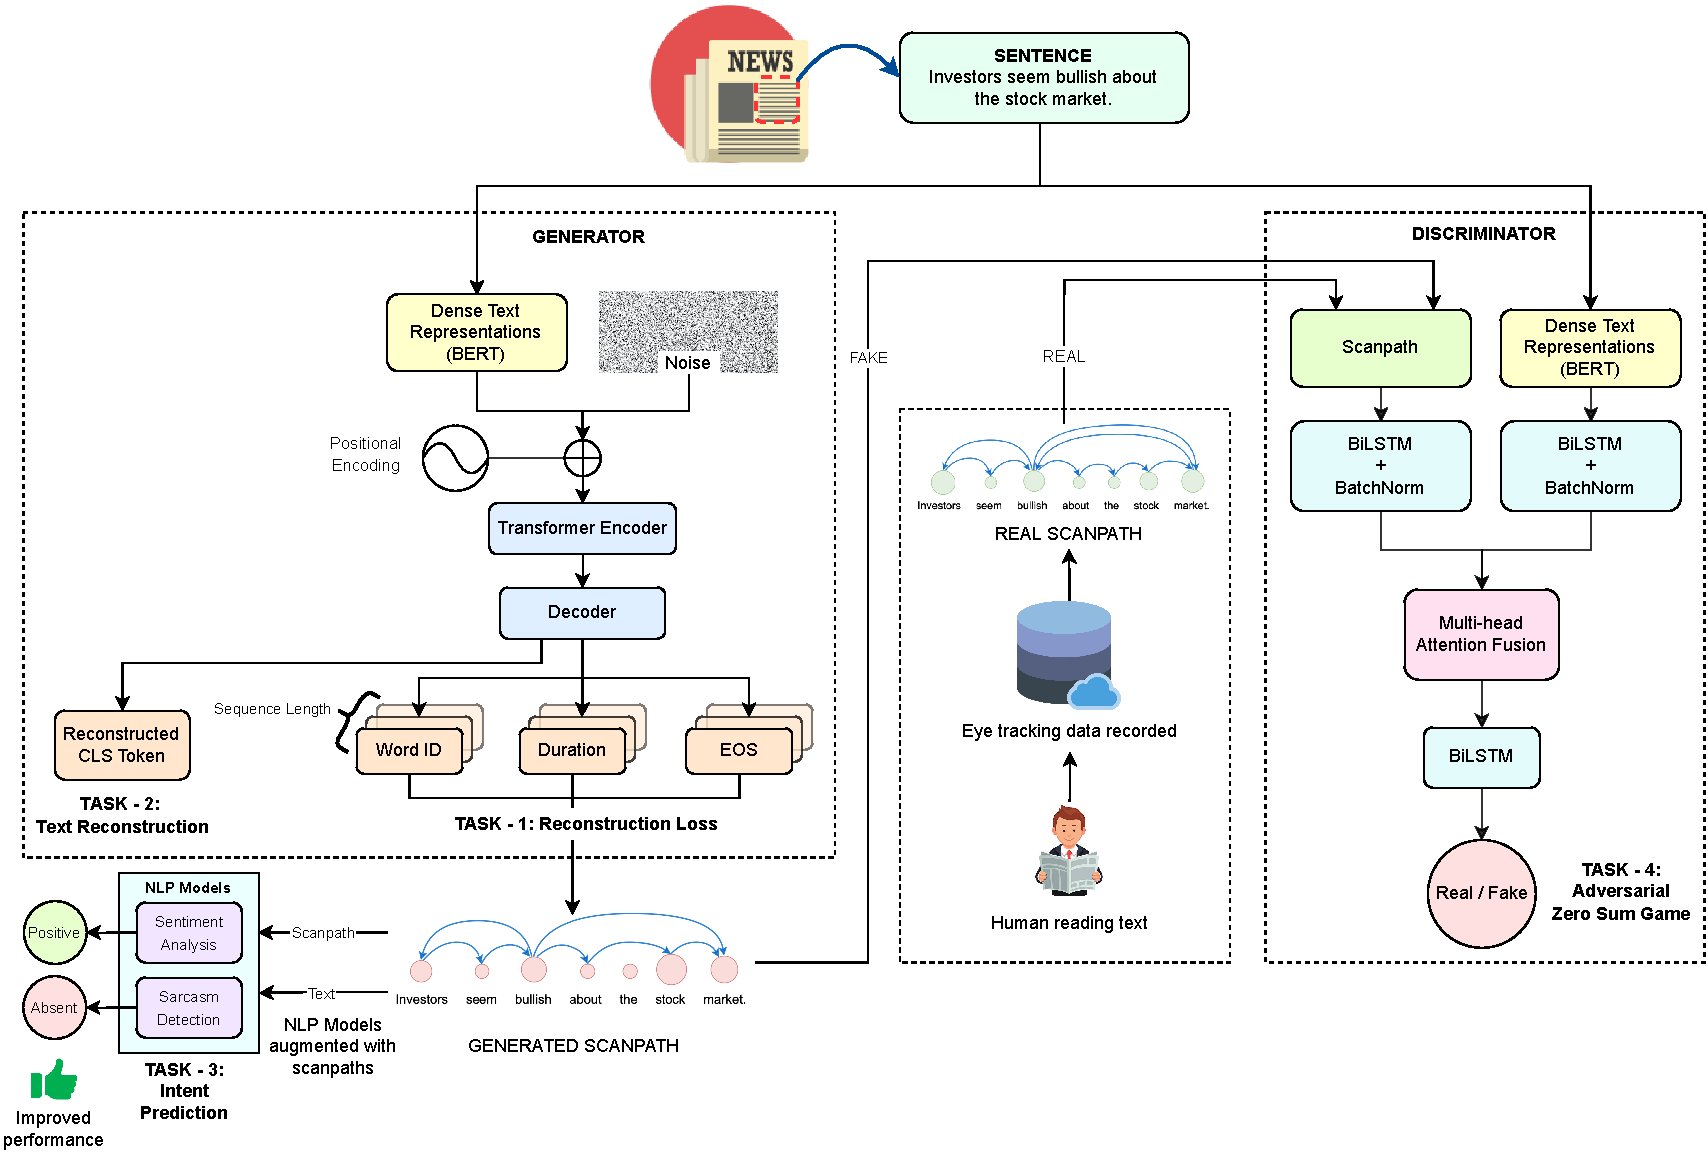
\includegraphics[width=\textwidth]{images/Intent_Scanpath_Figure.pdf}
    %\vspace*{-2mm}
    \caption{The architecture of the proposed Intent-Aware \textbf{ScanTextGAN} model. The model consists of a conditional generator and a discriminator playing a zero-sum game. Two cognitively inspired losses train the generator: scanpath (Task-1) and text (Task-2) reconstruction, a loss from the downstream intent of the natural language task (Task-3), and finally, the loss from the adversarial zero-sum game (Task-4). Variations of scanpaths are generated based on the downstream natural language task.}
    \label{fig:intent-model} 
%\vspace*{-5mm}
\end{figure*}


\begin{figure*}[]
%\vspace*{-2in}
    \centering
    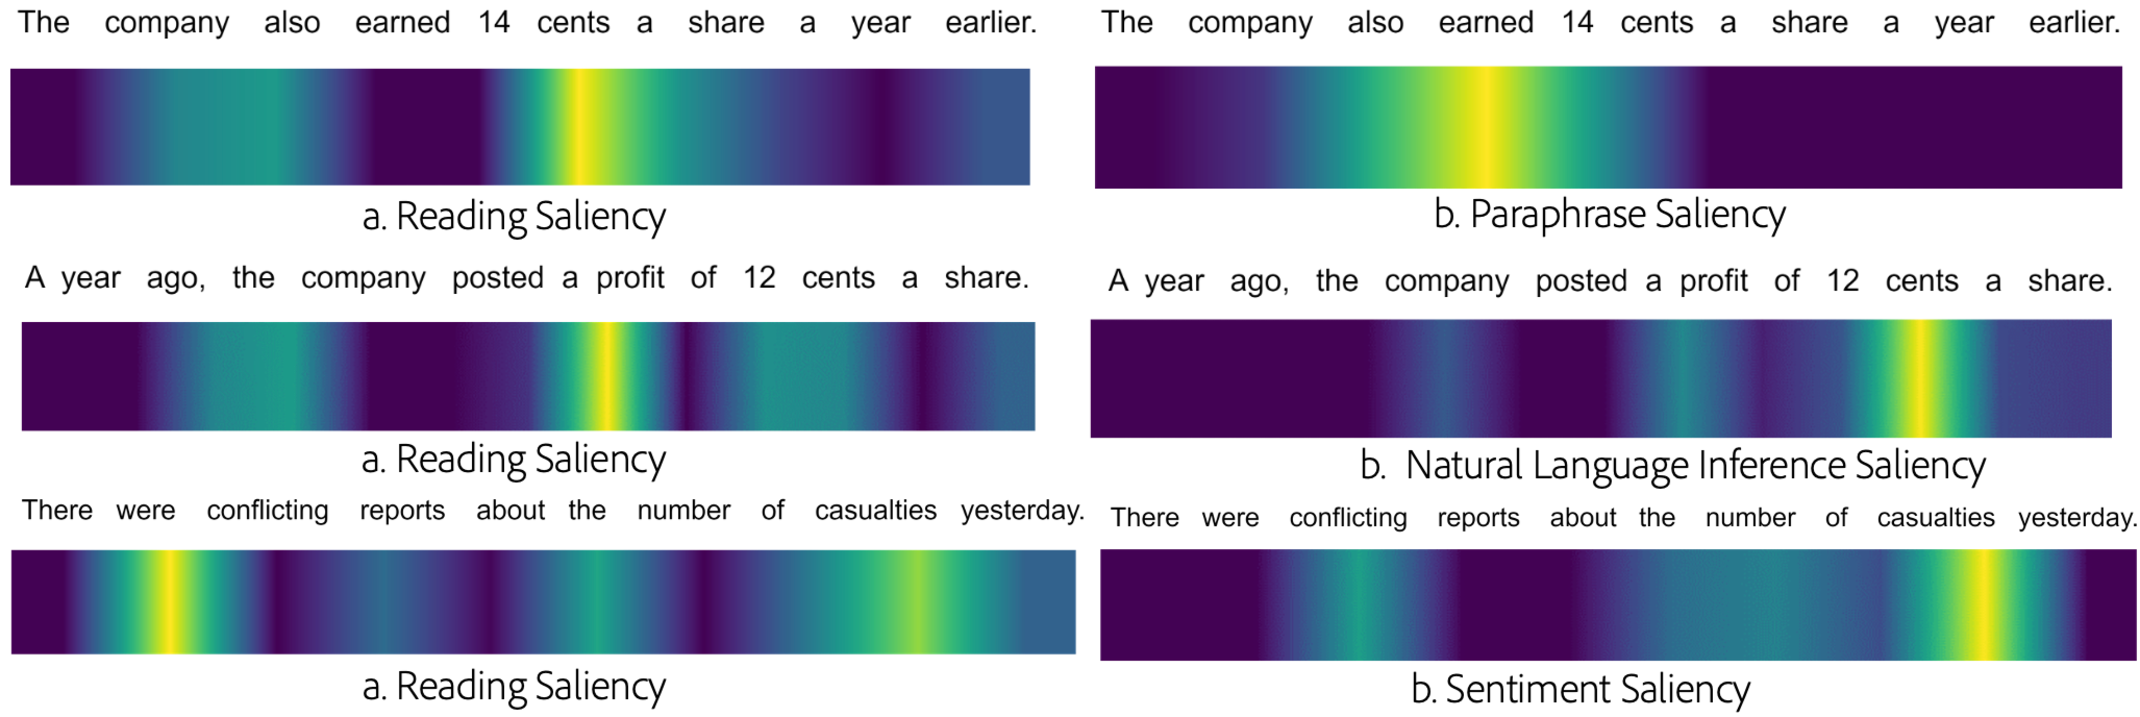
\includegraphics[width=\textwidth]{images/intent-scantextgan-saliency.pdf}
    %\vspace*{-2mm}
    \caption{Saliency samples generated by conditioning scanpath generation on different downstream natural language tasks. It can be observed that the conditioned saliency pays much more attention to words important for that downstream task.}
    \label{fig:intent-saliency-example} 
%\vspace*{-5mm}
\end{figure*}







\subsection{Conclusion}
\label{sec:ConclusionFutureWork}
In this work, we make two novel contributions toward integrating cognitive and natural language processing. (1) We introduce the first scanpath generation model over text, integrating a cognitive reading model with a data-driven approach to address the scarcity of human gaze data on text. (2)~We propose generated scanpaths that can be flexibly adapted to different NLP tasks without needing task-specific ground truth human gaze data. We show that both advances significantly improve performance across six NLP datasets over various baselines. Our findings demonstrate the feasibility and significant potential of combining cognitive and data-driven models for NLP tasks. Without the need for real-time gaze recordings, the potential research avenues for augmenting and understanding NLP models through the cognitive processing information encoded in synthesized scanpaths are multiplied.


\subsection{Limitations}
\label{Limitations}
In this work, we demonstrated artificial scanpath generation over multiple eye-tracking datasets. Further, our experiments build a link between cognitive and natural language processing and show how one can inform the other. However, the proposed method has a few limitations, which we aim to address in the future. The field needs work on bigger and more diverse eye-tracking datasets, which can enable scanpath generation over longer text sequences and can model generating scanpaths conditioned on previously read context. Besides, a better understanding of the entire scanpath generation process can help model the intra and inter-sentence scanpath generation process. The understanding would enable the integration of scanpaths to generative modeling tasks, which we intend to take up in future work. Another parallel direction is to include both explicit (like using RLHF) and implicit signals (like using cognitive signals) to better NLP tasks like language modeling.



